%%%%%%%%%%%%%%%%%%%%%%%%%%%%%%%%%%%%%%%%%%%%%%%%%%%%%%%%%%%%%%%%%%%%%%%%%%%%%%%%
%                         FORMATO DE TESIS UMSNH                               %
%%%%%%%%%%%%%%%%%%%%%%%%%%%%%%%%%%%%%%%%%%%%%%%%%%%%%%%%%%%%%%%%%%%%%%%%%%%%%%%%
% based on Harish Bhanderi's PhD/MPhil template, then Uni Cambridge
% http://www-h.eng.cam.ac.uk/help/tpl/textprocessing/ThesisStyle/
% corrected and extended in 2007 by Jakob Suckale, then MPI-iCBG PhD programme
% and made available through OpenWetWare.org - the free biology wiki
% forked from https://github.com/Tepexic/Tesis-UNAM on July 2017
% modifications made by Arturo Lopez Pineda

%                     Under GNU License v3

% ADAPTADO PARA UMSNH:  @arturolp

\documentclass[twoside,11pt]{Latex/Classes/thesisUMSNH}
%         PUEDEN INCLUIR EN ESTE ESPACIO LOS PAQUETES EXTRA, O BIEN, EN EL ARCHIVO "PhDthesisPSnPDF.cls" EN "./Latex/Classes/"
\usepackage{blindtext}                        % Para insertar texto dummy, de ejemplo, pues.
\usepackage[sort, numbers]{natbib}    % Personalizar la bibliografía a gusto de cada quien
\usepackage{url}
\usepackage{multirow}
% Note:
% The \blindtext or \Blindtext commands throughout this template generate dummy text
% to fill the template out. These commands should all be removed when 
% writing thesis content.
% This file contains macros that can be called up from connected TeX files
% It helps to summarise repeated code, e.g. figure insertion (see below).

%%%%%%%%%%%%%%%%%%%%%%%%%%%%%%%%%%%%%%%%%%%%%%
%            Colores de la UNAM              %
%%%%%%%%%%%%%%%%%%%%%%%%%%%%%%%%%%%%%%%%%%%%%%
% Para UNAN: Azul Pantone 541  -->(0,63,119) RGB
% Para UMSNH: PANTONE Blue 072 C
\definecolor{Azul}{RGB}{51,51,153}

% Para UNAM: Oro Pantone 460  -->(234,221,150) RGB
% Para UMNSH: PANTONE 110 C
\definecolor{Oro}{RGB}{204,153,51}


%%%%%%%%%%%%%%%%%%%%%%%%%%%%%%%%%%%%%%%%%%%%%%
%            Comandos para líneas            %
%%%%%%%%%%%%%%%%%%%%%%%%%%%%%%%%%%%%%%%%%%%%%%
%Se define un comando \colorvrule para hacer líneas verticales de color con 3 argumentos: color, ancho, alto
\newcommand{\colorvrule}[3]{
\begingroup\color{#1}\vrule width#2 height#3
\endgroup}

%Se define un comando \colorhrule para hacer líneas horizontales de color con 2 argumentos: color, ancho
\newcommand{\colorhrule}[2]{
\begingroup\color{#1}\hrule height#2
\endgroup}

%%%%%%%%%%%%%%%%%%%%%%%%%%%%%%%%%%%%%%%%%%%%%%
%          Comando para derivadas            %
%%%%%%%%%%%%%%%%%%%%%%%%%%%%%%%%%%%%%%%%%%%%%%
\newcommand{\derivada}[3][]{\ensuremath{\dfrac{\mbox{d}^{#1}#2}{\mbox{d}#3^{#1}}}} 
%primer argumento(opcional): orden de la derivada
%segundo argumento: función a derivar
%tercer argumento: variable respecto a la que se deriva


%%%%%%%%%%%%%%%%%%%%%%%%%%%%%%%%%%%%%%%%%%%%%%
%       Comando para la exponencial          %
%%%%%%%%%%%%%%%%%%%%%%%%%%%%%%%%%%%%%%%%%%%%%%
\newcommand{\e}[1][]{\ensuremath{\mbox{e}^{#1}}}
%primer argumento(opcional): exponente de la exponencial




% insert a centered figure with caption and description
% parameters 1:filename, 2:title, 3:description and label
\newcommand{\figuremacro}[3]{
	\begin{figure}[htbp]
		\centering
		\includegraphics[width=1\textwidth]{#1}
		\caption[#2]{\textbf{#2} - #3}
		\label{condicion}
	\end{figure}
}

% insert a centered figure with caption and description AND WIDTH
% parameters 1:filename, 2:title, 3:description and label, 4: textwidth
% textwidth 1 means as text, 0.5 means half the width of the text
\newcommand{\figuremacroW}[4]{
	\begin{figure}[htbp]
		\centering
		\includegraphics[width=#4\textwidth]{#1}
		\caption[#2]{\textbf{#2} - #3}
		\label{#1}
	\end{figure}
}

% inserts a figure with wrapped around text; only suitable for NARROW figs
% o is for outside on a double paged document; others: l, r, i(inside)
% text and figure will each be half of the document width
% note: long captions often crash with adjacent content; take care
% in general: above 2 macro produce more reliable layout
\newcommand{\figuremacroN}[3]{
	\begin{wrapfigure}{o}{0.5\textwidth}
		\centering
		\includegraphics[width=0.48\textwidth]{#1}
		\caption[#2]{{\small\textbf{#2} - #3}}
		\label{#1}
	\end{wrapfigure}
}

% predefined commands by Harish
\newcommand{\PdfPsText}[2]{
  \ifpdf
     #1
  \else
     #2
  \fi
}

\newcommand{\IncludeGraphicsH}[3]{
  \PdfPsText{\includegraphics[height=#2]{#1}}{\includegraphics[bb = #3, height=#2]{#1}}
}

\newcommand{\IncludeGraphicsW}[3]{
  \PdfPsText{\includegraphics[width=#2]{#1}}{\includegraphics[bb = #3, width=#2]{#1}}
}

\newcommand{\InsertFig}[3]{
  \begin{figure}[!htbp]
    \begin{center}
      \leavevmode
      #1
      \caption{#2}
      \label{#3}
    \end{center}
  \end{figure}
}







%%% Local Variables:
%%% mode: latex
%%% TeX-master: "~/Documents/LaTeX/CUEDThesisPSnPDF/thesis"
%%% End:
           % Archivo con funciones útiles
\usepackage[draft,inline,nomargin]{fixme} \fxsetup{theme=color}





%%%%%%%%%%%%%%%%%%%%%%%%%%%%%%%%%%%%%%%%%%%%%%%%%%%%%%%%%%%%%%%%%%%%%%%%%%%%%%%%
%                                   DATOS                                      %
%%%%%%%%%%%%%%%%%%%%%%%%%%%%%%%%%%%%%%%%%%%%%%%%%%%%%%%%%%%%%%%%%%%%%%%%%%%%%%%%
\title{Análisis estadístico del flujo de 1-gramas entre lenguajes indoeuropeos}
\author{JOSUÉ ELY MOLINA BECERRA} 
\facultad{FACULTAD DE CIENCIAS}                 % Nombre de la facultad/escuela
\escudofacultad{Latex/Classes/Escudos/fc_negro.pdf} % Aquí ponen la ruta y nombre del escudo de su facultad, actualmente, la carpeta Latex/Classes/Escudos cuenta con los siguientes escudos:
% "fi_azul" Facultad de ingenieria en color azul
% "fi_negro" Facultad de ingenieria en color negro
% "fc_azul" Facultad de ciencias en color azul
% "fc_negro" Facultad de ciencias en color negro
% Se agradecen sus aportaciones de escudos a jebus.velazquez@gmail.com

\degree{FÍSICO}       % Carrera
\director{CARLOS FRANCISCO PINEDA ZORRILLA}                   % Director de tesis
%\tutor{Nombre  Tutor }                    % Tutor de tesis, si aplica
\degreedate{2019}                                     % Año de la fecha del examen
\lugar{CIUDAD DE MÉXICO}                        % Lugar

\portadafalse                              % Portada en NEGRO, descomentar y comentar la línea siguiente si se quiere utilizar
%\portadatrue                                % Portada en COLOR



%% Opciones del posgrado (descomentar si las necesitan)
	%\posgradotrue                                                    
	%\programa{programa de maestría y doctorado en ingeniería}
	%\campo{Ingeniería Eléctrica - Control}
	%% En caso de que haya comité tutor
	%\comitetrue
	%\ctutoruno{Dr. Emmet L. Brown}
	%\ctutordos{Dr. El Doctor}
%% Datos del jurado                             
	%\presidente{Dr. 1}
	%\secretario{Dr. 2}
	%\vocal{Dr. 3}
	%\supuno{Dr. 4}
	%\supdos{Dr. 5}
	%\institucion{el Instituto de Ingeniería, UNAM}

\keywords{tesis,autor,tutor,etc}            % Palablas clave para los metadatos del PDF
\subject{tema_1,tema_2}                     % Tema para metadatos del PDF  

%%%%%%%%%%%%%%%%%%%%%%%%%%%%%%%%%%%%%%%%%%%%%%%%%%%%%
%                   PORTADA                         %
%%%%%%%%%%%%%%%%%%%%%%%%%%%%%%%%%%%%%%%%%%%%%%%%%%%%%
\begin{document}

\maketitle									% Se redefinió este comando en el archivo de la clase para generar automáticamente la portada a partir de los datos

%%%%%%%%%%%%%%%%%%%%%%%%%%%%%%%%%%%%%%%%%%%%%%%%%%%%%
%                  PRÓLOGO                          %
%%%%%%%%%%%%%%%%%%%%%%%%%%%%%%%%%%%%%%%%%%%%%%%%%%%%%
\frontmatter
\begin{acknowledgementspersonal}
	
Principalmente a mi abuela Nieves, por haberme cuidado y procurado tantos años sin ser su responsabilidad. 

\vspace{0.5cm}
A mis tios, padrinos y en muchas ocasiones mis padres, Dolores y Oscar; mis primas Flor y Yoalli, también Yurai. Gracias por apoyarme, aceptarme y darme una convivencia familiar.

\vspace{0.5cm}
A mi madre María de la Luz, por darme en mi niñez el aprecio a los libros y a la lectura; y porque en los últimos años, con su desinterés y su desconfianza, me enseñó a sólo depender en mi mismo. 

\vspace{0.5cm}
A mis primos Román, Alfonso y Sinar, por mostrarme que el trabajo duro nos lleva más lejos de la realidad donde nos toco nacer. 

\vspace{0.5cm}
A mi familia paterna, mis primos Liz, Carlos, Griss, Sandy, Elias, Martha y Yadi; mis tias Paty, Cata, Lupe y Xila; y a toda la \textit{Molinada sin fin}, por aceptarme dentro de una gran familia y por ayudarme a cumplir mi deseo.  

\vspace{0.5cm}
A Pamela, Diego, Zoé, Hilary y Yultzín, por ser mi mejor recuerdo de Fundación;  a Maffer, Cabral, Gaby y Alejandro por los \textit{buenos aires} del primer año de preparatoria; a Mauricio, Charly y Alex Califas por los mejores días en las canchas y en \textit{Potrero Dome}; a Brenda, Hodek y Kas \textit{Panda} por las platicas de humanidades, artes, historia y filosofía.  

\vspace{0.5cm}
Nuevamente a Pamela, Zoé, Maffer, Cabral, Mauricio y Charly, porque ustedes se han vuelto más que mis mejores amigos, gracias a ustedes y a sus familias por lo vivido y lo aprendido.

\vspace{0.5cm}
A Carla, por los años en la universidad en los que me mostró amistad, cariño y comprensión; por enseñarme a trabajar en equipo y también por llevarme a \textit{lo más alto y lo más bajo}.

\vspace{0.5cm}
A mis hermanos Carlos, Pavlos, George y Jack,  y a mi hermana Aila, porque ustedes son el mejor regalo y la mejor ilusión que el tiempo me brindó, y porque su existencia es la motivación para cruzar el mundo.

\vspace{0.5cm}
Finalmente a mi padre Carlos Molina Jiménez, porque su ausencia y su ejemplo, me hicieron ver que la formación académica no lo es todo,  y a la vez es la camino para superarnos y llegar a lo más alto. 


\end{acknowledgementspersonal}       % Comentar línea si no se usa
%\chapter*{}
%\pagenumbering{Roman}

\begin{acknowledgementsacademic}

Gracias a la UNAM por la formación académica recibida, y por el ejemplo profesional que me brindó en su personal, en la Preparatoria 9 con los profesores Norma Ramírez, Patricia Huerta, Elsa Cano, Arturo Palafox, José Carbajal y Arturo Jiménez; y en la Facultad de Ciencias con  Rosario Paredes, Patricia Goldstein, Pablo Barrera, Mirna Villavicencio, Valentín Porta, Ricardo Méndez, Roxana del Castillo y Catalina Stern. Gracias a todos por su labor, su ética y moral profesional,  y por todo el apoyo brindado. 

\vspace{0.5cm}
Gracias a todos los miembros del  grupo de idiomas, por formarme y enseñarme que se puede hacer física en las cosas más cotidianas, no sólo en los fenómenos abstractos. 

\vspace{0.5cm}
Gracias a mi asesor el Dr. Carlos Pineda, por sus consejos, su compresión, su apoyo y paciencia en las múltiples reuniones para elaborar este trabajo. También porque me enseño que en la ciencia,  lo más importante no son las formulaciones y los desarrollos complicados, sino la explicación y la sencillez con la que nos expresamos. 

\vspace{0.5cm}
Finalmente, gracias a los apoyos de los proyectos PAPIIT IG100518 y CONACYT CB-285754, ya que con ellos fue posible cada parte del desarrollo de está tesis. 

\end{acknowledgementsacademic}




   % Comentar línea si no se usa 
%% ******************************* Thesis Declaration ********************************

\begin{declaration}

Por la presente declaro que, salvo cuando se haga referencia específica al trabajo de otras personas, el contenido de esta tesis es original y no se ha presentado total o parcialmente para su consideración para cualquier otro título o grado en esta o cualquier otra Universidad. Esta tesis es resultado de mi propio trabajo y no incluye nada que sea el resultado de algún trabajo realizado en colaboración, salvo que se indique específicamente en el texto. 
% Author and date will be inserted automatically from thesis.tex


\end{declaration}
           % Comentar línea si no se usa

\begin{abstracts}        

En los últimos años, el desarrollo científico y tecnológico,  y el crecimiento económico de países como los Estados Unidos,  han hecho del idioma inglés el lenguaje común para la comunicación y para la difusión de información. Esto ha provocado que algunos vocablos del inglés comiencen a surgir en los demás idiomas,  mezclándose con las palabras típicas del idioma, y en ocasiones desplazándolas.  

Está tendencia no ha sido una característica única del inglés, a lo largo del tiempo, diferentes idiomas han aportado y modificado el vocabulario de otras lenguas. En este trabajo se estudia la forma en que los idiomas inglés, francés, alemán, italiano y español, se han relacionado durante el siglo XX a través de las palabras que son comunes entre ellos, llamadas  \textit{palabras migrantes};  y a partir de ellas, se han propuesto dos formas para cuantificar la influencia que un idioma ha tenido en otro. 

También se presenta un estudio estadístico llamado \textit{diversidad de rango}, con el que se cuantifican las distintas palabras migrantes que pueden ocupar lugar en un listado, si estas se ordenan  a partir de su frecuencia.  

Finalmente se justifica la falta de un rigor lingüístico, al eliminar cierta cantidad de palabras migrantes, para volver a obtener la influencia entre idiomas, y medir su similitud con los resultados previos. 



 
\end{abstracts}
%\end{abstractlongs}


% ----------------------------------------------------------------------                   % Comentar línea si no se usa

%%%%%%%%%%%%%%%%%%%%%%%%%%%%%%%%%%%%%%%%%%%%%%%%%%%%%
%                   ÍNDICES                         %
%%%%%%%%%%%%%%%%%%%%%%%%%%%%%%%%%%%%%%%%%%%%%%%%%%%%%
%Esta sección genera el índice
\setcounter{secnumdepth}{3} % organisational level that receives a numbers
\setcounter{tocdepth}{3}    % print table of contents for level 3
\tableofcontents            % Genera el índice 
%: ----------------------- list of figures/tables ------------------------
\listoffigures              % Genera el ínidce de figuras, comentar línea si no se usa
\listoftables               % Genera índice de tablas, comentar línea si no se usa


%%%%%%%%%%%%%%%%%%%%%%%%%%%%%%%%%%%%%%%%%%%%%%%%%%%%%
%                   CONTENIDO                       %
%%%%%%%%%%%%%%%%%%%%%%%%%%%%%%%%%%%%%%%%%%%%%%%%%%%%%
% the main text starts here with the introduction, 1st chapter,...
\mainmatter
\def\baselinestretch{1.5}                   % Interlineado de 1.5

% this file is called up by thesis.tex
% content in this file will be fed into the main document
%----------------------- introduction file header -----------------------
%%%%%%%%%%%%%%%%%%%%%%%%%%%%%%%%%%%%%%%%%%%%%%%%%%%%%%%%%%%%%%%%%%%%%%%%%
%  Capítulo 1: Introducción- DEFINIR OBJETIVOS DE LA TESIS              %
%%%%%%%%%%%%%%%%%%%%%%%%%%%%%%%%%%%%%%%%%%%%%%%%%%%%%%%%%%%%%%%%%%%%%%%%%

\chapter{Introducción}


\section{La base de datos y su interpretación} % section headings are 

Para la elaboración del trabajo,  se dispuso de la base de datos de los los n-grams de Google Books. Esta base de datos tiene hasta el momento alrededor del 4$\%$ de todas las publicaciones en diferentes idiomas,  y se caracteriza por en listar  por cada año y por cada idioma de publicación los “n-gramas” más utilizados.   Los n-gramas son las palabras o conjunto de palabras que forman el texto de un libro, donde el número n indicará la cantidad de palabras que forman el grama.  Es decir, los  1-grama son palabras individuales (una sola palabra o un signo), los 2-grama son frases compuestas por dos 1-grama, los 3-grama el conjunto de tres 1-grama y así sucesivamente.   Con la herramienta del \textit{n-gram viewer} \cite{ngramv}, los usuarios pueden acceder a una forma visual el comportamiento a lo largo del tiempo de un n-grama en los diferentes idiomas en que se publicó.  

A partir de esta base, se extrajeron los datos de los 1-grama en cinco diferentes idiomas, inglés, francés, alemán, italiano y español, correspondientes a las publicaciones de 269 años (1740-2009).  De acuerdo a \cite{iplosone},  el kernel de un idioma lo componen entre 1500 a 3000 palabras más comunes del mismo,  cantidad que basta para conocer al idioma.  Para el estudio del trabajo se tomaron por cada año y por cada idioma,  las cinco mil palabras más usadas (cantidad que abarca palabras dentro y fuera del kernel), teniendo conjuntos homogéneos en tamaño.

Cada palabra está asociada a una frecuencia, que es la cantidad de veces que apareció una palabra en las publicaciones de un año y un idioma, y asu vez cada frecuencia se vincula a un rango, que es la posición que ocupa la palabra en un ordenamiento.  Cada listado, está ordenado en forma descendente a partir de la frecuencia de cada palabra,  ocupando la posición uno y rango uno la palabra más frecuente, la posición dos y rango dos la segunda más frecuente y así sucesivamente, entonces las palabras más usadas tienen una frecuencia mayor y un rango menor. 

Para aclarar y familiarizar los términos, se utilizara la palabra popularidad para auxiliar la relación entre la frecuencia y el rango, de esta manera las palabras más populares son las más frecuentes.



\section{Forma de búsqueda}

Se identifican palabras que sean iguales en escritura, carácter por carácter y que estén presentes en dos o más idiomas.  Si se define como  \textbf{Migración}, al movimiento de palabras de un idioma a otro, entonces las palabras \textbf{Palabras Migrantes}  son aquellas que están presentes en al menos dos idiomas.  Conviene en este punto realizar dos definiciones que serán útiles.

\hfill \break

Se define como  \textbf{idioma origen}, al idioma en el cual la palabra apareció por primera vez dentro de la lista de las cinco mil palabras más usadas.  

\hfill \break 

Se define como i\textbf{idioma receptor}, a  aquel donde la palabra está presente, siendo un conjunto diferente al idioma origen.  

\hfill \break

Para que existan las palabras migrantes, se necesita un origen y al menos un receptor. Si una palabra está presente en más de dos idiomas, alguno es el origen y los demás son los receptores. 

Una vez que se tiene certeza de cuáles palabras son migrantes, y en cuáles idiomas está presente se procede a determinar el idioma origen y los idiomas receptores.   Si se suponen dos idiomas A y B donde la palabra se encuentra, y se sabe con seguridad el año de aparición en cada idioma y el rango que ocupó para ese año,  el criterio para determinar el origen es el siguiente: 


\begin{enumerate}
	
	\item  Si la palabra apareció en años anteriores en el idioma A (dentro de las 5 mil más usadas) que en el idioma B, se establece al idioma A como el idioma origen y B como el receptor.
	
	\item Si la palabra apareció en el mismo año en ambos idiomas, se establece el idioma origen a aquel donde la palabra tuvo un menor rango, es decir, si el rango en la lista de las más usadas en el idioma A es menor que el rango en la lista del idioma B, entonces A es el idioma origen, en caso contrario, el origen es B.
\end{enumerate}

Los dos argumentos anteriores, se pueden ampliar si la palabra está presente en tres o más idiomas. Un análisis detallado de las palabras que cumplen esta condición se cubrirá en las secciones posteriores.

La manera de clasificar el idioma origen de las palabras puede carecer de otras pautas para ser más preciso, sin embargo, a lo largo de toda la investigación se optó por utilizar lo más posible los datos de los n-gramas y  con ellos crear reglas para obtener resultados.  Una forma más precisa sería tomando otro tipo de base de datos, con información etimológica de las palabras y las diferentes escrituras que tomó la palabra hasta que prevaleció con una estructura escrita.  

Conocidos los idiomas origen y receptor de las palabras migrantes, se llamarán \textbf{Préstamos} a las palabras con un mismo origen y que están  presentes en un receptor.  Se llamaran como los préstamos de A en B, a las palabras con origen A y receptor B. 


\subsubsection*{Ventajas}


\begin{itemize}
	
	\item [$-$] Determina el idioma donde la palabra fue más popular al comienzo de la base de datos (1740), y hacia donde se esparció el vocablo, dando un carácter histórico de los idiomas mas populares en diferentes épocas. 
	
	\item [$-$] Localiza las palabras que conservaron su escritura al pasar de un idioma a otro. 
	
	\item [$-$] Toma como influencia a las palabras que son importantes en un idioma y que son transmitidas a los demás, en ocasiones el origen deja de ser influyente, y el idioma que lleva las palabras a otros receptores, es también un receptor.  Este punto y el anterior se trataran a detalle en las secciones siguientes. 
	
\end{itemize}


\subsubsection*{Desventajas}


\begin{itemize}
	
	\item [$-$] Al encontrar palabras con igual escritura, se obtienen casos donde el significado en cada idioma es diferente.  Por ejemplo, la palabra  \textit{MAYOR}, que está presente en el inglés y en el español,  significa alcalde en inglés, mientras que en español es más grande que.
	
	\item [$-$] No se localizan palabras que han sufrido transformaciones en la escritura al pasar de un idioma a otro, consecuente de que la palabra se adapta a la gramática de los diferentes idiomas receptores.  Por ejemplo, las palabras imagine e imaginar, son similares en los primeros caracteres, teniendo el mismo significado en el inglés y en el español, no obstante la terminación de  sus últimas letras se modificó al estar en  la lengua inglesa y la española. 
	
	\item [$-$] Define un origen distinto al verdadero.  Muchos de estos casos se presentan al no tener una base de datos con más idiomas, y el verdadero origen puede estar en estas exclusiones. Por ejemplo la palabra natural, que proviene del latín y se encuentra en inglés y español,  el programa la identifica como  de origen inglés, más su verdadera procedencia es el latín. 
	
\end{itemize}


\newpage

\section{Primeros objetivos del análisis}

Una premisa que puede explicar el por qué las palabras se alteran o no al pasar de un idioma a otro, se puede vincular a la adaptabilidad de la palabra por parte de los hablantes de la lengua.  Por ejemplo, la palabra \textit{internet} con un claro origen en el inglés, y año de “invención” alrededor de 1990,  migró y cobró relevancia en otros idiomas por la facilidad y la rapidez con la que las sociedades  aprovecharon el fenómeno de internet, beneficiándose de la revolución que trajo en aspectos como el desarrollo de las telecomunicaciones,  el avance tecnológico,  la sofisticación de aparatos, el cambio positivo en el modo de vivir de las personas, entre otros beneficios.  Tal adaptación por parte de la sociedad hizo cotidiano el concepto, y en consecuencia la palabra.  

Otro palabra que sirve como ejemplo para este razonamiento es \textit{wi-fi}, donde la mayoría de las personas entiende el significado y el concepto que describe la palabra. Probablemente  exista una traducción para describir al fenómeno en cada idioma, sin embargo la cotidianidad que existe entre la escritura original y la comunidad que lo emplea, hace inviable una modificación que resulte en la pérdida de la familiaridad.


Un caso donde un concepto y fenómeno ha logrado un cambio en la forma de vida de las comunidades,  y la palabra que se asocia a él ha sido transformada por los receptores es el del \textit{teléfono}; su escritura original \textit{teletrofono} es proveniente del italiano,  pero su apogeo se dio en el inglés, modificando la escritura a \textit{telephone}; los diferentes idiomas también hicieron una modificación, siendo \textit{téléphone} en francés, \textit{telefon} en alemán, \textit{teléfono} en español, e incluso el italiano adopta la escritura del español   (el n-gram viewer es útil para comprobar esto), a pesar de ser el idioma origen. Pocos cuestionan el cambio que originó el teléfono en la sociedad desde su aparición hasta  tiempos recientes, pero contrario al internet su escritura no prevaleció.  

El tiempo que le toma a las palabras el pasar de un idioma a otro, es un factor que influye en la prevalencia de las palabras. El ejemplo del internet en los años recientes,  donde  la globalización ha permitido que la información pase de un medio a otro con mayor fluidez y el fenómeno que conlleva la palabra sea asimilado por las diferentes comunidades en un tiempo relativamente corto entre el origen de la palabra y su uso en los demás idiomas. 

El encontrar factores o sucesos  que expliquen el por qué las palabras fluyen de un lado a otro, será uno de los objetivos del trabajo. Más objetivos se irán planteando conforme se avance en el texto, para llegar al propósito del análisis, permitiendo establecer una forma de cuantificar la influencia entre los idiomas. Antes de llegar a este punto, habrá que hacer más clasificaciones para un mejor manejo de los datos. 

\newpage

\section{Clasificaciones de las palabras}

La primera clasificación  hecha fue el identificar  el  idioma origen y los diferentes idiomas receptores para las palabras migrantes, para establecer los préstamos de un idioma en otro, tras esta organización de datos, y como primer paso para llegar a la influencia de una lengua sobre otra,  es útil conocer qué tan importantes han sido los préstamos de un mismo origen en los demás idiomas, y también en qué año o años un idioma receptor ha adoptado recibido más préstamos de diferentes orígenes. 

Si se supone un idioma receptor B, un año cualquiera que esté dentro de los datos y  la lista  de las 5 mil palabras más usadas de B para tal año, entonces dentro del registro habrá préstamos con idioma  origen A en alguna posición de rango.  Estos préstamos se han clasificado como:


\begin{description}

	\item [Préstamos Nuevos:] Son palabras que aparecen por primera vez en las más usadas del idioma B.
	
	\item [Préstamos Repetidos:] Palabras que ya habían aparecido en alguna lista del idioma B, y para ese año lo volvieron a hacer.
	
	\item [Préstamos Acumulados:] Conjunto de préstamos nuevos y repetidos.
	
	
\end{description}


Por lo tanto para un determinado año dentro de la lista de las más usadas, existirán palabras que aparecieron en la lista por primera vez y palabras que ya habían estado en la lista en al menos un año anterior.  Asimismo  habrá años en los que no existieron préstamos nuevos,  por lo que todos los préstamos por año serán repetidos.

Ya que la base de datos de los N-grams de Google es amplia, muchas palabras pueden estar mal clasificadas o mal contadas, al existir errores en la tipografía o en las clasificaciones de los libros.  Para consolidar que las palabras que migran son relevantes en el idioma receptor, se han eliminado palabras que se presentan como nuevas en un año y que nunca más volvieron a aparecer en las listas de los años posteriores,  con el propósito de deslindarse de errores tipográficos, en consecuencia todas  las palabras que se clasificaron al principio como préstamos nuevos, pasaron a ser en algún momento préstamos repetidos. 

Las palabras de acuerdo a  \cite{contenidopal}, se clasifican en palabras funcionales que auxilian a las demás a estructurar un mensaje de acuerdo a la gramática del idioma, y en palabras de contenido que llevan la información y significado del mensaje. Para obtener la esencia de las palabras que fluyen entre los idiomas, se han eliminado de las listas a los artículos, preposiciones y conjunciones, correspondientes a las palabras funcionales, quedando solo palabras de contenido.  Al tratarse de cinco diferentes idiomas, las posibles palabras funcionales se obtuvieron de diferentes diccionarios y páginas \cite{englishdic, frenchdic, germandic, italiandic, spanishdic}.

En secciones posteriores, se realizará un estudio sobre el cómo afecta a los resultados la eliminación de palabras a partir de reglas arbitrarias.  Por el momento todo el trabajo se apoya en la eliminación de las palabras funcionales.


\section{Migración directa y por puente}

Se había tratado anteriormente como determinar el origen y los receptores de las palabras migrantes, una vez clasificados como préstamos, se propone el siguiente caso: 
Un idioma origen A, tiene préstamos en los idiomas B y C,  es decir hay al menos una palabra proveniente de A y que está tanto en B como en C; las preguntas que surgen son las siguientes: ¿cómo se trasladaron los préstamos a los diferentes receptores? y ¿los préstamos han sido más importantes en los receptores que en el propio idioma origen. 

Para responder estas interrogantes, se piensa en un préstamo con origen A  que apareció en C y antes que en B. De las listas de las palabras más usadas correspondientes a los 5 años previos a la aparición en B,  se toman  los promedios de las posiciones de rango que ocupó  la palabra  en los listados de A y de C, con ellos hay dos posibles formas de migración:


\begin{description}
	
	\item[Migración Directa:] El promedio de los rangos en A es mayor que en C. La palabra migró de A a C y de A a B de forma independiente. 
	
	\item[Migración por puente:] El promedio en C es mayor que en A. La palabra necesito a C para poder llegar a B
	
\end{description}


Se tomaron los 5 años anteriores, ya que al ser palabras publicadas en libros, la información transmiten tarda en ser asimilada por una población, no es tan rápida como lo puede ser la información transmitida por los periódicos. Por lo que debe existir un preámbulo de tiempo en lo que un libro es leído y un autor publica sobre el.

Si entre los años de aparición en B y en C hay menos de 5 años, entonces se toma el promedio en los rangos en la cantidad de años de esa diferencia.

Uno de los resultados esperados con las migraciones a través de los puentes es observar en qué idiomas receptores la popularidad de los préstamos fue mayor que en el idioma origen. Aumenta la complejidad, al tener un préstamo en más de dos idiomas receptores, en cada caso se repitió el algoritmo en cada idioma intermedio. 

El encontrar y asegurar las posibles formas en las que una palabra se trasladó a todos los idiomas en los que está presente,  requiere de las relaciones con otro tipo de datos de diferentes categorías, como la política, la economía, la cultura, etc. Por el momento, al solo tener la base de datos de los N-grams, se tratará de utilizarla lo máximo posible.  En el capítulo 4, se discutirá la importancia de las palabras que utilizan un puente. 

\newpage
\section{Interpretación de la influencia}

El medir la influencia que un evento tiene sobre otro, no es un proceso que esté mecanizado, como lo puede ser el determinar la distancia entre dos puntos o evaluar el tamaño de un objeto.  No existe un conjunto de reglas que afirmen o refuten si un acontecimiento es influyente en otro. En cada evento existe una cantidad diferente de variantes que intervienen entre ellas para  conducir a una respuesta sobre la influencia. 

En el caso de los idiomas, las variables que se conocen son el tiempo (manifestado en los años de las listas), la frecuencia y el rango de las palabras.  Un dato importante es que la cantidad de libros que fueron digitalizados es mayor en los últimos años que en los primeros,  la frecuencia de la palabra con rango uno en las lista de 1740 puede ser la diezmilésima parte de la del mismo rango en la lista de 2009, inclusive tratándose de la misma palabra,  entonces se tendrán que normalizar los datos para que tengan la misma proporción. 

De nuevo, se piensa en los préstamos de A, y los de C que están presentes en B.  Una manera preliminar de conocer la influencia, es contar cuántos préstamos de cada idioma están en las listas de cada año en B,  y el idioma más influyente será el que tenga más elementos. La idea es buena, pero no suficiente, para demostrarlo, se piensa en la lista de un año en B,  y al contar los préstamos, se obtiene una cantidad X para los que tienen origen A y  una cantidad Y para los de origen C,  con X $>$ Y. 

Al utilizar el criterio anterior,  el idioma A es en principio más influyente que el C por tener más cantidad de elementos en B, pero si los préstamos de C ocupan rangos más pequeños que los de A, como el tener un rango pequeño es similar a tener una frecuencia mayor,  si se suma cada frecuencia  de los préstamos de A y C,  la suma para las de C puede ser mayor que la suma para las de A, en consecuencia las palabras de C son más importantes dentro de B que las palabras de A, ya que son más frecuentadas o son utilizadas más veces.   

El utilizar la frecuencia es otra herramienta con la que se logra sustentar la respuesta a la influencia, puede ser alternativa o complementaria a la basada en la cantidad, en el trabajo se empleara cada una para describir un caso particular, aún falta añadir la normalización,  de manera formal se describen los dos métodos y se recuerda que las listas son de las cinco mil palabras más usadas. 

\begin{description}
	
	\item[Influencia por cantidad:] Se toma como influencia a la cantidad de préstamos de A en la lista de un año en B.
	
	\item[Influencia por frecuencia:] La influencia estará determinada por relacion porcentual entre las frecuencias de los préstamos de A en la lista de B y la frecuencia de todas las palabras de la lista de B. 
	
\end{description}


Para entender mejor  la influencia por frecuencia, se describira a detalle el algoritmo empleado:

\begin{enumerate}
	
	\item En un año determinado del idioma B, se sumarán las frecuencias $f_{t}$ de cada una de las cinco mil palabras más usadas.  Esta cantidad se llamará \textbf{frecuencia  total por año.}
	
	\begin{equation}
	\label{ec.ftot}
	f_{t} = \sum_{i=1}^{5000} f_{i} \,\,\,\,\,\,\,\,\, i = posici\'{o}n \,\,\, de \,\,\,cada \,\,\,palabra
	\end{equation}
	
	\item Como se conocen las posiciones $j$,  que ocupan los préstamos A en la lista de B, se procede a sumar sólo las frecuencias asociadas a estas palabras. Esta cantidad será la \textbf{frecuencia de préstamo} $f_{p}$,  esta cantidad es siempre menor que la frecuencia total por año.
	
	\begin{equation}
	\label{ec.fpres}
	f_{p} = \sum_{j} f_{j} \,\,\,\,\,\,\,\,\, j = posici\'{o}n \,\,\, de \,\,\,cada \,\,\,prestamo
	\end{equation}
	
	
	\item  Se divide la frecuencia de préstamo entre la frecuencia total por año, esta cantidad es la indicada para medir la influencia, se denotará como \textbf{frecuencia de uso} $F$ y es la porción que representan las frecuencias de los préstamos de A en B.  Como la influencia por cantidad se expresa como un porcentaje,  bastará multiplicar el cociente por cien para obtener el porcentaje.  
	
	\begin{equation}
	\label{ec.fuso}
	F = \frac{f_{p}}{f_{t}} * 100
	\end{equation}
	
	
	Entre más cercana a 100 $\%$ sea la frecuencia de uso, los préstamos del idioma A serán más relevantes en B.
	
	
\end{enumerate}


La frecuencia de uso está ya normalizada, siendo el parámetro de normalización la frecuencia total por año. Otra posible normalización sería al considerar la cantidad de libros que fueron registrados para obtener la lista de las palabras más usadas en cada año,  sin embargo se desconoce esta cifra.  


\newpage
\section{La influencia en 109 años (1900-2009)}

Se ha comentado anteriormente la descripción de la base de datos extraída y la forma en la que se han clasificado los datos para ser adecuados en la medición de la influencia.  Al ser limitada la base de datos por no tener registros ( con suficiente información) para los cinco idiomas (inglés, francés, alemán, italiano y español) antes de 1740,  existe un periodo de tiempo durante los primeros treinta o cincuenta años, donde se encuentran una mayor cantidad de préstamos de un idioma a otro; este fenómeno se sigue presentando si el año del comienzo de las mediciones se recorre.  Este periodo con las mayores migraciones en los primeros años, presenta ruido a las mediciones de la influencia, mostrando una mayor influencia (en cantidad o en frecuencia)  en los años iniciales que en los finales.

Para evitar tener ruido en las mediciones, se decidió partir la información en dos conjuntos, que ayuden al análisis, el primero será el conjunto base comprendido desde 1740 hasta 1900, y el segundo será el conjunto búsqueda englobado entre 1901 y 2009.  Con ello,  los préstamos y sus clasificaciones encontradas (para cualesquiera idiomas) en el conjunto base  se tomaron como verdaderas,  obteniendo un “background” de las palabras que migraron de un lado a otro  antes del comienzo de las mediciones en el conjunto búsqueda, evitando así el ruido.  Dada las particiones, la medición de la influencia solo se realizó en el conjunto búsqueda.

Como se tienen dos maneras de medir influencia,  hay casos en los que conviene utilizar solo una forma o ambas.  Para los préstamos nuevos, se decidió emplear el método de influencia por cantidad, ya que mostrara los años de mayor intercambio de palabras que se asientan en el idioma receptor; el método de influencia por frecuencia no proporciona información relevante en estos préstamos ya que el impacto que representan las palabras nuevas en la frecuencia de uso del idioma receptor es muy pequeña, ya que generalmente las palabras nuevas entran a las listas en posiciones muy altas de rango.  

La influencia por frecuencia brinda mayor información si se emplea en los préstamos por año, al evaluar la relevancia de todos los préstamos del idioma origen en el receptor. En este punto es importante el background que se obtuvo del conjunto base, ya que también se contó la influencia de los préstamos acumulados que surgieron en el background, debido a que para el primer año del conjunto búsqueda (1901) ya forman parte del idioma receptor, y tienen un impacto en él. 

De manera resumida se hicieron por el momento dos análisis, el primero obteniendo la influencia por cantidad de los préstamos entre dos idiomas entre 1901 y 2009, y el segundo al contabilizar la influencia por frecuencia de los préstamos acumulados durante los mismos años.  Los resultados de cada prueba se presentarán en las siguientes secciones. 


            % ~10 páginas - Explicar el propósito de la tesis
\chapter{La base de datos}

\fxnote{En el titulo del capitulo, solo la primera palabra tiene mayusculas, 
a menos que sea un nombre, etc. Ya la cambie, pero revisa en otross
capitulos, que la capitalizacion este bien.}

\section{La base de datos y su interpretación} % {{{

Para la elaboración del trabajo,  se dispuso de la base de datos de los los
$n$-grams de Google Books  \cite{ngramv} \fxnote{Acá tienes que citar}. Esta base de datos
tiene hasta el momento alrededor del 4$\%$ de todas las publicaciones en
diferentes idiomas,  y se caracteriza por en listar  por cada año y por cada
idioma de publicación los ``$n$-gramas'' \fxnote{Mira como se ponen las
comillas en LaTex. Es un poco latoso y sin sentido, pero asi es. Otra
correccion: como $n$ representa un número, prefiero escribir $n$-gramas a
$n$-gramas. Nota el cambio en el símbolo.} más utilizados.   Los $n$-gramas son
las palabras o conjunto de palabras que forman el texto de un libro, donde el
número $n$ indicará la cantidad de palabras que forman el grama.  Es decir, los
1-grama son palabras individuales (una sola palabra o un signo), los 2-gramas
son frases compuestas por dos 1-gramas, los 3-gramas el conjunto de tres 1-gramas
y así sucesivamente.   Con la herramienta del \textit{n-gram viewer}
\cite{ngramv}, los usuarios pueden acceder a una forma visual el comportamiento
a lo largo del tiempo de un $n$-grama en los diferentes idiomas en que se
publicó.  

A partir de esta base, se extrajeron los datos de los 1-grama en cinco
diferentes idiomas, inglés, francés, alemán, italiano y español,
correspondientes a las publicaciones de 269 años (1740-2009).  De acuerdo a
\cite{languagesascool},  el kernel de un idioma lo componen entre 1500 a 3000 palabras
más comunes del mismo,  cantidad que basta para conocer al idioma~\fxnote{Este no es  el claim. Reformula}.  Para el
estudio del trabajo se tomaron por cada año y por cada idioma,  las cinco mil
palabras más usadas (cantidad que abarca palabras dentro y fuera del kernel),
teniendo conjuntos homogéneos en tamaño.

Cada palabra está asociada a una frecuencia, que es la cantidad de veces en que
que la  palabra apareció en las publicaciones de un año y un idioma, y a su vez
cada frecuencia se vincula a un rango, que es la posición en un ordenamiento.
Cada listado está ordenado de manera descendente en la frecuencia y de manera
ascendente en el rango, la palabra más utilizada tendrá mayor frecuencia y le
corresponde el rango uno,  la siguiente será la segunda más frecuente
correspondiente al rango dos,  la tercera más frecuente con rango tres y así
sucesivamente para todos los elementos.  Con ello se afirma que las palabras
más usadas tienen una mayor frecuencia y un rango menor. 

% }}}
\section{Palabras comunes entre idiomas}
 % {{{
\fxnote{Creo que el nombre de esta sección no es acertado. Tambien me gustaria
que dijeras por que vas a ahcer lo qeu vas a hacer. }

Al tratar de identificar como es la presencia de un idioma en otro, una de las formas para lograrlo es reconocer aquellas palabras que son comunes entre dos o más idiomas,  estas representarán la base de toda la investigación al ser una herramienta para determinar como se han relacionado y alterado los idiomas por la presencia de nuevos vocablos.  Para ello se identifican palabras que sean iguales en escritura, carácter por carácter y
que estén presentes en dos o más idiomas.  Si se define como
\textbf{migración}, al movimiento de palabras de un idioma a otro, entonces las
\textbf{palabras migrantes}  son aquellas que están presentes en al
menos dos idiomas\fxnote{no debes capitalizar las deficiones, proque no son nombres
propios}.  

Conviene en este punto realizar dos definiciones que serán
útiles.
% \hfill \break
\fxnote{Acá pusiste un hfill y un break. Para que? Los comenté porque no 
les encuentro sentido. }
\begin{itemize}
\item 
Se define como  \textbf{idioma origen}, al idioma en el cual la palabra
apareció por primera vez dentro de la lista de las cinco mil palabras más
usadas.  

% \hfill \break 
\item 
Se define como \textbf{idioma receptor}, a  aquel donde la palabra está
presente, siendo un conjunto diferente al idioma origen.  
\end{itemize}

% \hfill \break

Para que existan las palabras migrantes, se necesita un origen y al menos un
receptor. Si una palabra está presente en más de dos idiomas, alguno es el
origen y los demás son los receptores. 

Una vez que se tiene certeza de cuáles palabras son migrantes, y en cuáles
idiomas está presente se procede a determinar el idioma origen y los idiomas
receptores.   Si se suponen dos idiomas $\textit{A}$ y $\textit{B}$  donde la
palabra se encuentra, y se sabe con seguridad el año de aparición en cada
idioma y el rango que ocupó para ese año,  el criterio para determinar el
origen es el siguiente: 
\begin{enumerate}
\item  Si la palabra apareció en años anteriores en el idioma $\textit{A}$
(dentro de las 5 mil más usadas) que en el idioma $\textit{B}$ , se establece
al idioma $\textit{A}$  como el idioma origen y $\textit{B}$  como el receptor.
\item Si la palabra apareció en el mismo año en ambos idiomas, se establece el
idioma origen a aquel donde la palabra tuvo un menor rango, es decir, si el
rango en la lista de las más usadas en el idioma $\textit{A}$  es menor que el
rango en la lista del idioma $\textit{B}$ , entonces $\textit{A}$  es el idioma
origen, en caso contrario, el origen es $\textit{B}$ .
\item Se descartan palabras que contengan un solo carácter, las que son
compuestas por letras y números y aquellas que aparecen en el receptor sólo en un año. La intención es tener una  nueva base de datos con el mayor contenido
limpio con palabras que perduran al menos dos años en el receptor.

\end{enumerate}
\fxnote{Creo que convendría tener un par de ejemplos, como tablas o algo asi, 
que incluyan palabras que migran razonablemente y otras que no, para uqe se entienda
las limitaciones de la definicion. Esto recuerda que dio mucha lata.}
Los argumentos anteriores, se pueden ampliar si la palabra está presente en
tres o más.

% \newpage
\fxnote{Aca pusiste un newpage. Este tipo de comandos normalmente no se usan. }
La manera de clasificar el idioma origen de las palabras puede carecer de otras
pautas para ser más preciso, sin embargo, a lo largo de toda la investigación
se optó por utilizar lo más posible los datos de los $n$-gramas y  con ellos
crear reglas para obtener resultados.  Una forma más precisa sería tomando otro
tipo de base de datos, con información etimológica de las palabras y las
diferentes escrituras que tomó la palabra hasta que prevaleció una estructura.  

Conocidos los idiomas origen y receptor de las palabras migrantes, se llamarán
\textbf{préstamos} a las palabras con un mismo origen y que están  presentes en
un receptor.  Un receptor $\textit{B}$, puede tener palabras con diferentes
orígenes $\textit{A}$, $\textit{C}$ o $\textit{D}$, también una palabra con
origen $\textit{A}$ puede llegar a diferentes receptores.  Los préstamos de
$\textit{A}$  en $\textit{B}$  son el conjunto de palabras con origen
$\textit{A}$  y con receptor $\textit{B}$.     





%\subsubsection*{Ventajas}
\fxnote{Esto no es una subsubseccion. Redacta mejor algo que introduzca la lista. 
Tambien quité la linea, para que seas homogeneo cuando ahces una lista. Si quieres
cambiar el simbolo del item en todas las listas, mejor si lo haces de manera global. 
debe haber una forma de hacerlo.}

Los criterios empleados para establecer orígenes ha mostrado mayormente resultados adecuados, sin embargo se presentaron donde el algoritmo no logra asentar el origen adecuado. Dentro de las ventajas ($\bullet$) y desventajas ($\ast$) del método se encuentran las siguientes:

\begin{itemize}
\item [$\bullet$] 
% [$-$] 
Determina el idioma donde la palabra fue más popular al comienzo de
la base de datos (1740), y hacia donde se esparció el vocablo, dando un
carácter histórico de los idiomas mas populares en diferentes épocas. 

\item [$\bullet$] 
Localiza las palabras que conservaron su escritura al pasar de un
idioma a otro. 

\item [$\bullet$] 
Valora a un idioma como importante e influyente si sus vocablos son
transmitidos a los demás y perduran por un periodo de tiempo. También el mismo
idioma es influyente si a través de él se han esparcido palabras a los demás, a
pesar de que no sea el idioma origen. 

\item [$\ast$] Al encontrar palabras con igual escritura, se obtienen casos donde
el significado en cada idioma es diferente.  Por ejemplo, la palabra
$\textit{mayor}$, que está presente en el inglés y en el español,  significa
alcalde en inglés, mientras que en español es más grande que.

\item [$\ast$]
No se localizan palabras que han sufrido transformaciones en la
escritura al pasar de un idioma a otro, consecuente de que la palabra se adapta
a la gramática de los diferentes receptores.  Por ejemplo, las palabras
$\textit{imagine}$ e $\textit{imaginar}$, son similares en los primeros
caracteres, teniendo el mismo significado en el inglés y en el español, no
obstante la terminación de  sus últimas letras se modificó al estar en  la
lengua inglesa y la española. 

\item [$\ast$]
 Puede definir un origen distinto al verdadero.  Muchos de estos casos se
presentan al no tener una base de datos con más idiomas, y el verdadero origen
puede estar en estas exclusiones. Por ejemplo la palabra natural, que proviene
del latín y se encuentra en inglés y español con igual escritura,  el programa
la identifica proveniente del inglés, más su verdadera procedencia es el latín. 

\end{itemize}

Se han revisado las palabras encontradas con el algoritmo descrito, en su
mayoría los resultados son aceptables. Los mayores inconvenientes resultaron al
clasificar las palabras y las migraciones entre idiomas de la misma familia
lingüística.  En los capítulos siguientes se proporcionara un vinculo para
poder observar todas las palabras encontradas. \fxnote{Ok, veo que pones algunos ejemplos. 
Discutamos si ponemos algo aca como una tabla o no.}


Las palabras que se encontraron se pueden agrupar en dos conjuntos de acuerdo a\cite{contenidopal}, las \textbf{palabras funcionales} son aquellas que auxilian a las demás a estructurar un mensaje de acuerdo a la gramática del idioma, y las \textbf{palabras de contenido} son las que llevan la información y el significado del mensaje. Ya  que se busca tener palabras cuyo significado refleje un concepto o situación donde estas son utilizadas, se decidio eliminar de las listas a los artículos, pronombres, preposiciones y conjunciones, correspondientes a las palabras funcionales, quedando solo palabras de contenido. Para eliminar las posibles palabras funcionales se emplearon diferentes paginas y diccionarios especializados en cada lengua \cite{englishdic, frenchdic, germandic, italiandic, spanishdic}. 

\fxnote{no entiendo 
que uso le das a las italicas y al bold face. Me puedes por favor aclarar eso?}

\fxnote{yo hbaia puesto las italicas y en negritas para remarcar el concepto de palabras funcionales y de contenido. }


\section{Partición de datos} % {{{

\fxnote{No entiendo esta seccion }

-
El tener una base de datos que comprende 269 años (1740-2009) no garantiza ser lo suficientemente completa para determinar el año preciso en que una palabra apareció en otro idioma, hay palabras cuyo primer empleo es más antiguo que el primer año en que se tienen registros. Este tipo de palabras tienen una característica común y es que migran en los primeros treinta años, sin importar el año en que comiencen las mediciones; a pesar de ser una característica importante el flujo de palabras siempre es mayor en este periodo, posterior a el las migraciones son menos frecuentes. Para estabilizar 
el flujo de palabras, se decidió partir la información en dos conjuntos que cuyo contenido se emplee de forma diferente y se complemente uno a otro.  Se llamarán como:


\textbf{Conjunto base.} (1740-1889) Todas las migraciones que ocurran dentro de estos años se tomarán como verdaderas, obteniendo un antecedente o historial de las palabras que migraron de un lado a otro y se han asentado en el idioma receptor. Con ello se establece una base de las palabras que ya forman parte de un receptor y que son relevantes al estar en las listas de sus palabras mas comunes. 

\textbf{Conjunto de búsqueda.} (1900-2009) Las migraciones en estos años se cuestionarán tratando de dar un significado al por que ha ocurrido el movimiento,  siendo en este periodo las migraciones más estables. Para las posteriores técnicas se utilizará siempre al conjunto de búsqueda.
% }}}



\chapter{Palabras nuevas}

% Intro {{{
En el capítulo anterior se mencionó que el algoritmo toma como  idioma
influyente a aquel que transmite palabras hacia los demás y que estas perduren
en los receptores al menos dos años.   El objetivo ahora es identificar qué
idioma es más influyente sobre los demás, sin embargo establecer un método que
proporcione este resultado no es sencillo,  puede ser ambiguo decir que algo es
influyente, no hay una manera de seguir una serie de pasos que finalicen en
decir si algo es influyente o no,  o cuánta influencia se tuvo en el proceso.
Incluso que un idioma transmita palabras no es criterio suficiente para afirmar
una influencia.  

Al tener una base de datos  con los préstamos de un idioma en otro,  una primer
manera de establecer la influencia es  identificar los tiempos donde ocurren
las migraciones.  Para ello conviene hacer una clasificación dentro de los
propios préstamos y a partir de ella  continuar con una cuantificación de la
influencia.  Si se tiene una pareja de idioma origen \textit{A} e idioma
receptor \textit{B} entonces se clasifican a los préstamos de \textit{A} en
\textit{B} como:

\textbf{Préstamos Nuevos}: Son palabras que aparecen por primera vez en las más
usadas del idioma \textit{B}.  Únicamente serán nuevos en el primer año de
aparición,  es fundamental tener certeza del año en que ocurrió la migración. 

Se recuerda que todos los préstamos nuevos, volvieron a aparecer en alguna
lista del idioma B posterior al primer año de la migración, omitiendo a
aquellos que solo aparecieron una vez. 

Entonces dentro de los años comprendidos en el conjunto de búsqueda
(1901-2009), existen múltiples posibilidades con las cuáles trabajar a los
cinco idiomas. La manera en que se tratara de llegar a un resultado que muestre
la influencia puede ser de tres formas:
\begin{enumerate}
\item Contando por cada año los préstamos de origen A que están presentes en
los diferentes receptores.
\item Tomar ahora a \textit{A} como el idioma receptor, y contando cuántos
préstamos nuevos de los diferentes orígenes están presentes en cada año. 
\item Tomando fijos un idioma \textit{A} y un idioma \textit{B},  contabilizar
cuántos préstamos nuevos por año se encuentran si se toma a \textit{A} como
origen y a \textit{B} como receptor,  una vez hecho esto  repetir el conteo
intercambiando a \textit{B} como el origen y a \textit{A} como el receptor. 
\end{enumerate}


En los tres casos la influencia estará ligada a la cantidad de préstamos
nuevos.  Las tres formas son correctas y servirán para decir en cual idioma
receptor  el origen \textit{A} ha sido más influyente por haber mayor cantidad
de migraciones; también cuál ha sido el idioma  que más ha influido en
\textit{A} y finalmente entre dos idiomas,  cuál ha influenciado más al otro. 
% }}}
\section{Eventos que ayudan a las migraciones} % {{{

Una parte complementaria de interpretar la influencia es responder qué es lo
que propicia el haber migraciones de un lado hacia otro.  El tener los
préstamos nuevos clasificados por el año de la primera migración ayuda a
identificar posibles causas de carácter histórico que propiciaron las
migraciones en ese año o alrededor de él.  Por ejemplo, la globalización en los
años recientes ha propiciado que una ola de palabras de su campo semántico
hayan migrado entre orígenes y receptores,  \textit{internet},
\textit{computadora}, \textit{web}, \textit{email},  \textit{software}, son
ejemplos de palabras que surgieron tras el fenómeno de globalización. 

Los eventos pueden ser de diferentes tipos y al tratar con idiomas, se espera
que en tales eventos participen países, personajes o  comunidades que hablan
las lenguas involucradas.  El asociar sucesos con palabras y a la vez con
determinados grupos ayudará a mostrar el alcance que tuvo un lenguaje y la
forma en la que surgió la influencia y esta se propagó. 

Como el conjunto de búsqueda abarca 109 años,  la propagación de las palabras
no es inmediata, en diferentes épocas las migraciones ocurrieron de distintas
formas,  por ejemplo, en 1900 la información no circulaba tan rápido como se
hace actualmente, un evento de esta época puede tener repercusiones en cinco,
diez o más años,  dependiendo de factores geográficos, económicos, tecnológicos
y  la  propia relevancia del evento en las demás comunidades.

En cada resultado posterior, se hizo una investigación histórica de las
palabras que conforman los préstamos nuevos entre idiomas,  en la mayor parte
de los casos se ubicaron sucesos para explicar el por qué ciertas palabras
migraron y la importancia del año o años en que lo hicieron. 

% }}}
\section{Búsqueda y lectura de palabras nuevas} % {{{

Ya establecida la forma en que se buscarán  palabras nuevas en los diferentes
idiomas,  los resultados encontrados se presentarán de la siguiente manera:
\begin{itemize}
\item Por cada idioma se determinó la influencia que esté ejerció en los demás,
mencionada en el punto 1 al comienzo del capítulo.   Ya que se el proceso fue
para todos los idiomas,  al ver primero la influencia de \textit{A} sobre
\textit{B}  (y los demás),  en el siguiente resultado se estará cubriendo la
influencia  de \textit{B}  sobre \textit{A} , cubriendo así el punto 2. 
\item La cuantificación de la influencia por los préstamos nuevos se realizó en
el periodo de 109 años (1900 - 2009) y por cada década comprendida en estos
años, es decir por una parte se mostrarán la cantidad de palabras que
aparecieron en los 109 años y por otra parte como se distribuye esta cantidad
en las diferentes décadas.  La intención de este punto es observar en qué
periodos un idioma aportó (recibió) más  hacia (de) los demás.
\item Se proporcionará en \cite{prestamos_nuevos} las listas  de préstamos
nuevos entre cada idioma, agrupados por el año de aparición en el receptor.  Se
especificará en el Anexo 1  la forma de leer e interpretar estas listas.
\item En cada resultado mostrado se agregara un resultado general para la
influencia en los 109 años, y un contexto detallado entre las migraciones hacia
un idioma receptor por década,  enfatizando los sucesos históricos de las
palabras involucradas, así como los posibles detonantes que propiciaron los
movimientos. 
\item Cada análisis tendrá comentarios sobre el punto 3,  las gráficas
correspondientes se anexaran en el apéndice 1.
\end{itemize}

\subsection*{Lectura de las gráficas} % {{{

Para las gráficas del trabajo se utilizaron diferentes colores para
caracterizar las influencias de un idioma, además en cada gráfica se especifica
los idiomas que intervienen y para su mejor lectura se utilizaron
abreviaciones. Los colores y abreviaciones de cada idioma son:

\fxnote{Porfa aprende a hacer tablas, y haz una tabla acá}

inglés   $\,\,\,\,\,\, \rightarrow \,\,\,$   EN   $\,\,\,\rightarrow\,\,\,$  azul

francés  $\,\,\,       \rightarrow \,\,\,$   FR   $\,\,\,\rightarrow\,\,\,$  amarillo

alemán   $\,\,\,       \rightarrow \,\,\,$   GE   $\,\,\,\rightarrow\,\,\,$  violeta

italiano $\,\,          \rightarrow \,\,\,$  IT   $\,\,\,\,\,\rightarrow\,\,\,$  verde

español  $\,\,\,       \rightarrow \,\,\,$  SP   $\,\,\,\rightarrow\,\,\,$  guinda



En cada grafica se especificará por medio de  abreviaciones y  colores a los
idiomas tratados, todo ello en una leyenda; la primera abreviación que será el
idioma origen de los préstamos, y la segunda corresponderá al idioma receptor,
por ejemplo  la leyenda EN-FR serán los préstamos que van del inglés al
francés, en cambio FR-EN son los préstamos que van en sentido contrario

En todas las gráficas, el eje horizontal está representado por los años del
conjunto de búsqueda 1900-2009,  mientras que en el eje vertical se presenta la
cantidad de prestamos nuevos. 
% }}}
% }}}
\section{Palabras nuevas de un idioma en los demás} % {{{
\subsection{Inglés} % {{{

\begin{figure} % {{{
	\begin{center}
		\begin{subfigure}
			[Inglés por siglo.]{
			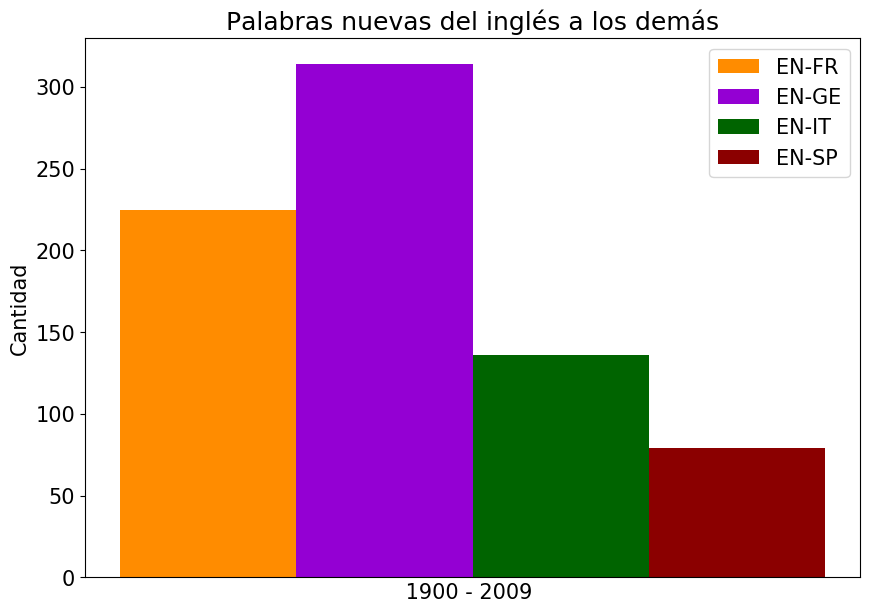
\includegraphics[scale=.4]{Cap_3/ICS_a_EN.png}
			\label{fig.ICS_a_EN}}
		\end{subfigure}
	
	\vspace{0.5cm}
	
		\begin{subfigure}
			[Inglés por década.]{
			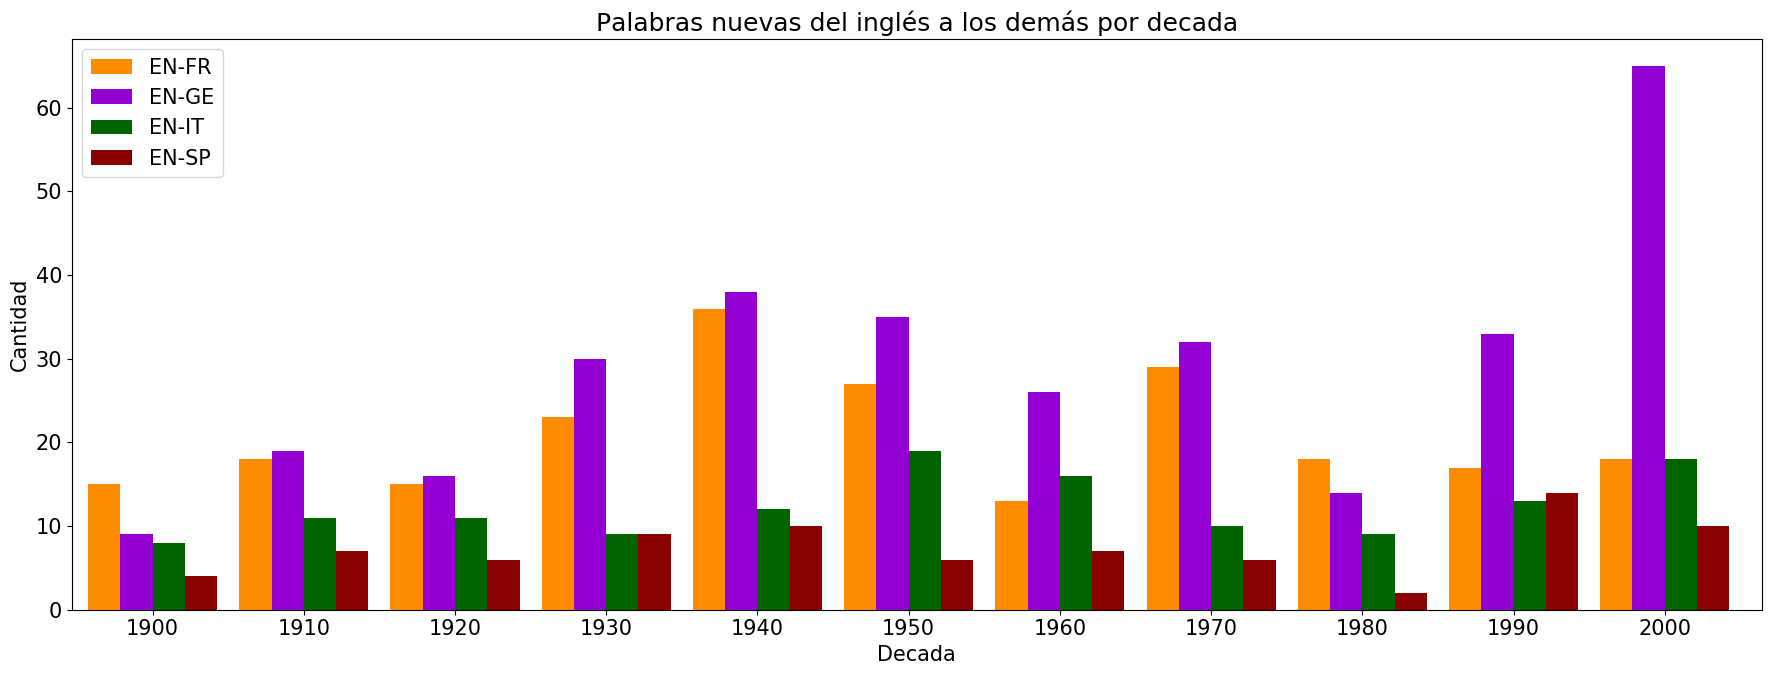
\includegraphics[width=14cm, height=7cm]{Cap_3/ICD_a_EN.png}
			\label{fig.ICD_a_EN}}
		\end{subfigure}
	
	\caption{Palabras nuevas del inglés en los demás.}
	\label{fig.IC_EN}
	\end{center}
\end{figure} % }}}

De manera general, el idioma que más se ha beneficiado del inglés ha sido el
alemán, con 300 préstamos en 100 años.  Inglés y alemán forman parte de la
misma familia lingüística de las lenguas germánicas,  posible razón de los
mayores intercambios. Entre las lenguas romances, el francés fue el más
favorecido, pero también es la más similar por las relaciones normandas entre
ambas.
\subsubsection*{Inglés-Francés} % {{{

Los mayores aportes se dieron de 1930 a 1970, periodo que engloba comienzos de
la gran depresión, la segunda guerra mundial y la guerra fria, sucesos donde
participaron países de ambas lenguas. Las palabras involucradas en este periodo
hacen referencia a estos eventos, entre 1944 y 1945 surgieron en el francés los
términos \textit{Churchill}, \textit{territories}, \textit{nazis} y
\textit{catastrophe},  mientras que en las décadas entre 1950 y 1970
aparecieron \textit{Nixon}, \textit{dollar} y \textit{Johnson}; dos de estas
palabras aluden a apellidos de presidentes de los Estados Unidos,  Lyndon B.
Johnson y Richard Nixon, cuyos periodos de gobierno fueron  entre 1963-1969 y
1969-1974 respectivamente.
% }}}
\subsubsection*{Inglés-Alemán} % {{{
Entre todas las décadas, solo en dos de ellas (1900  y 1980) el alemán no fue
el idioma que mas prestamos recibió  del ingles. Entre las palabras encontradas
en las demás épocas están \textit{economic} (1929), \textit{depression} (1931),
\textit{investment} (1933), \textit{Roosevelt} (1935), que pertenecen al campo
semántico de la gran depresión mientras que el presidente Franklin D. Roosevelt
gobernó posterior a la crisis económica y durante la segunda guerra mundial. La
gran depresión se origino en los Estados Unidos con consecuencias en la
economía de diferentes países, entre ellos  Alemania, y fue uno de los motivos
que propiciaron la segunda guerra mundial.

En las ultimas dos décadas, la globalización y  el desarrollo tecnológico son
responsables del mayor crecimiento, palabras como \textit{standards} (1983),
\textit{market} (1994), \textit{internet} (1996), \textit{economy} (1996),
\textit{online} (1998), \textit{value} (2001), \textit{financial} (2003) y
\textit{customer} (2007). 
% }}}
\subsubsection*{Inglés-Italiano} % {{{
La principal característica de las palabras hacia el italiano son apellidos de
personajes involucrados en la segunda guerra mundial, \textit{Roosevelt} (1941)
o \textit{Stalin} (1949), el el caso de Joseph Stalin a pesar de que su
nacionalidad no es la de algún pais de habla inglesa, en el ingles su apellido
tomo notoriedad para exportarse a los otros idiomas; este es un ejemplo de que
no todas las palabras encontradas nacieron en el idioma origen,  solamente en
el se hicieron populares.  En los últimos años nuevamente la globalización y el
poder economico de los Estados Unidos han hecho favorable el crecimiento del
ingles, \textit{internet} (1996), \textit{bussines} (2000), \textit{marketing}
(2001) y \textit{bush} (2002), son terminos que abarcan estos acontecimientos. 
% }}}
\subsubsection*{Inglés-Español} % {{{
El español ha sido en la mayor parte de los periodos de diez años,  el idioma
que menos prestamos ha adoptado del ingles, sin embargo los hechos a los que se
han ligado han sido en más areas que en las otras combinaciones.  Nombres de
organizaciones y empresas,  \textit{standard} (1933) (y \textit{oil} (1931)
aludiendo a la extinta Standard Oil) y \textit{unesco} (1955);  personajes de
la historia de los Estados Unidos,  \textit{Roosevelt} (1941), \textit{Kennedy}
(1961), \textit{Johnson} (1966),  \textit{Nixon} (1972) y \textit{Bush} (1990);
y a la globalizacion en los últimos 20 años, \textit{internet} (1996),
\textit{mail} (1999), \textit{marketing} (2001) y \textit{software} (2004).   

A pesar de no ser el idioma más favorecido es al que en más areas ha impregnado
el ingles, siendo este un factor que también puede indicar una mayor
influencia,  en cuantas áreas esta presente un idioma y que tanto se utiliza. 

% }}}
% }}}
\subsection{Francés} % {{{

\begin{figure} % {{{
	\begin{center}
		\begin{subfigure}
			[Francés por siglo.]{
				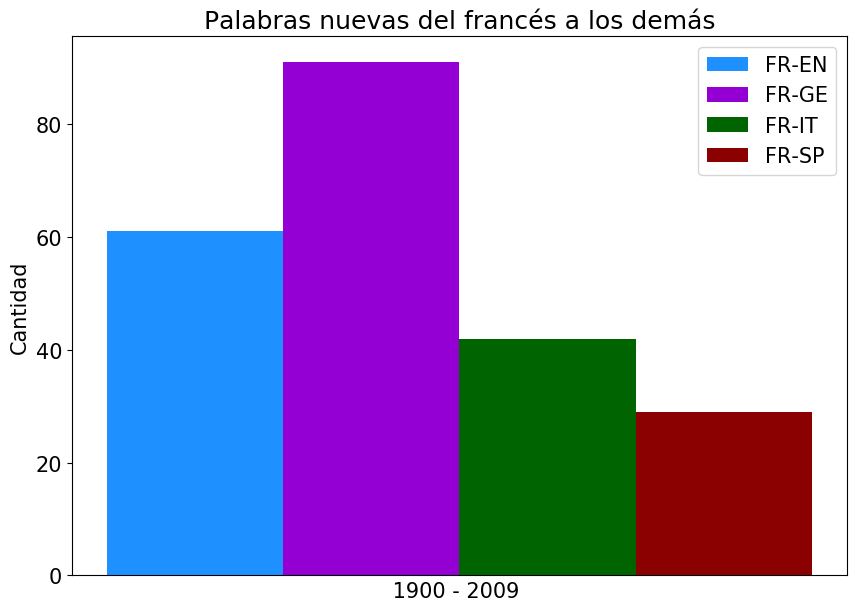
\includegraphics[scale=.4]{Cap_3/ICS_a_FR.png}
				\label{fig.ICS_a_FR}}
		\end{subfigure}
		
		\vspace{0.5cm}
		
		\begin{subfigure}
			[Francés por década.]{
				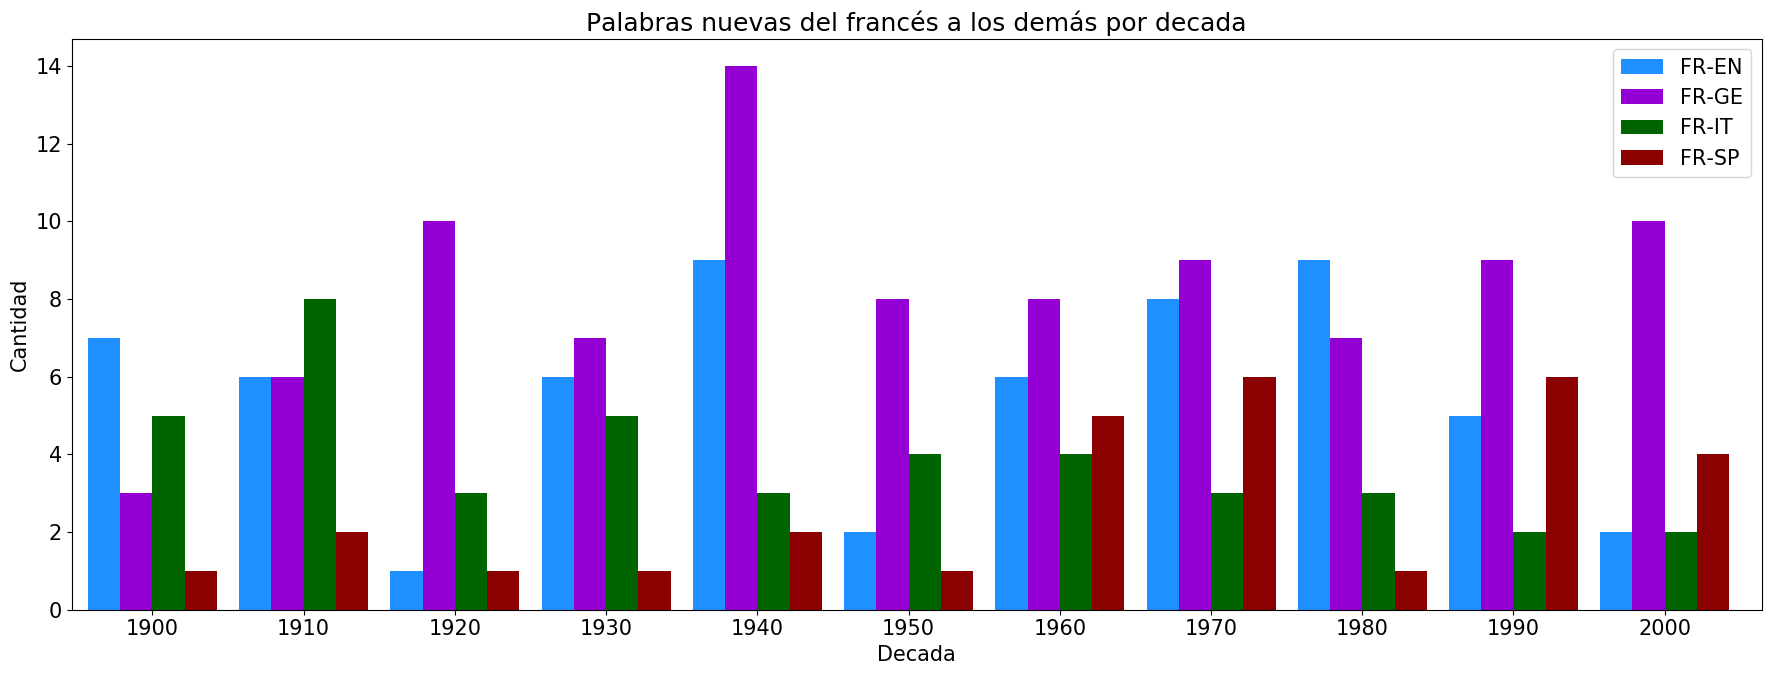
\includegraphics[width=14cm, height=7cm]{Cap_3/ICD_a_FR.png}
				\label{fig.ICD_a_FR}}
		\end{subfigure}
		
		\caption{Palabras nuevas del francés en los demás.}
		\label{fig.IC_FR}
	\end{center}
\end{figure} % }}}


A lo largo del siglo pasado (y primeros años del actual), el alemán se ha
beneficiado de elementos del francés más que los otros, adoptando más del doble
que el español a pesar de ser un idioma de la misma familia. Una posible razón
del por qué el alemán ha sido donde han llegado la mayor cantidad de palabras
es que etimológicamente el francés es más parecido a los otros, y el mayor
aporte a los demás ocurrió antes de 1900.  También es importante destacar que
el papel del francés en 1800 era tan relevante como lo es ahora el inglés,
donde la mayor cantidad de obras eran publicadas en este idioma.

\subsubsection*{Francés-Inglés}% {{{

La característica de los prestamos, es que son principalmente palabras que son comunes en el ingles, y que a simple vista serian catalogados como errores de clasificación, por ejemplo  \textit{diagnostic,} \textit{clients,} \textit{placement,} \textit{adaptation,} \textit{diffusion,} \textit{amplitude,} no pareciese lógico ver que migraron del francés hacia el inglés, sin embargo el algoritmo designo este origen por ser al principio de la base de datos (1740)  donde las palabras eran más utilizadas.  Antes de considerarse un error, se puede inferir que antes las obras en francés eran bastas de vocablos de otros idiomas, destacando el papel que tuvo el francés como idioma "común" para transmitir información. 


% }}}
\subsubsection*{Francés-Alemán}% {{{

De la grafica \ref{fig.ICD_a_FR}, el alemán tuvo dos décadas donde la diferencia de palabras nuevas que llegaron a él es mas significativa que en los otros idiomas, en los periodos de 1920 y 1940  (posteriores a las dos guerras mundiales), entre el contenido se ubicaron a  textit{diplomatie} (1917), \textit{bourgeoisie} (1919),  \textit{guerre} (1925), \textit{Allemagne} (1925), \textit{Russie} (1925) y \textit{empire} (1937); siendo un conjunto de palabras utilizables al referise a temas políticos  o diplomáticos, y por donde participaron países hablantes de las dos lenguas. 


% }}}
\subsubsection*{Francés-Italiano}% {{{

El italiano se vio mas susceptible al francés en los primeros años del siglo, aunque no fue posible ligar a las palabras a un hecho relevante en estos años. Entre las pocas clasificaciones se encuentra la terna cientica con \textit{Poincaré} (1924), apellido del matemático francés Henri Poincaré, y la bélica,  entre los terminos encontrados estan \textit{Versailles} (1924), textit{Vietnam} (1966)  y \textit{URSS} (1975), mostrando que la  La primera y segunda guerra mundial fueron detonantes para el flujo de palabras.


% }}}
\subsubsection*{Francés-Español}% {{{

Al igual que la tendencia en el italiano, en el español no llegaron gran cantidad de palabras cuyo contenido sea ligado a un evento, a pesar de que en cien años migraron alrededor de veinte. La mas destacada fue \textit{euros} (2002) por ser el año de circulación de la moneda de la unión europea, organización donde son miembros países importantes de las dos lenguas. 

El hecho de no poder enlazar palabras a eventos, no significa que el francés no es importante para el español (o el italiano), sino que el periodo donde los hechos tuvieron mayor impacto no esta dentro del periodo de búsqueda,  por ejemplo hechos como la revolución francesa, o la invasión napoleónica a España, propiciaron a un mayor intercambio en este sentido, pero al ocurrir antes de 1900 no permite tener una conclusión de ello. 


% }}}
% }}}
\subsection{Alemán}% {{{

\begin{figure} % {{{
	\begin{center}
		\begin{subfigure}
			[Alemán por siglo.]{
				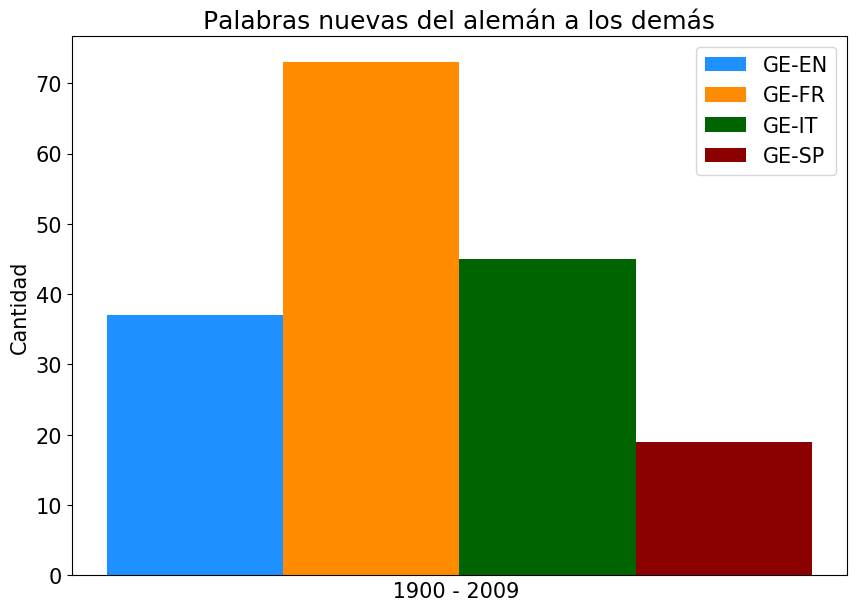
\includegraphics[scale=.4]{Cap_3/ICS_a_GE.png}
				\label{fig.ICS_a_GE}}
		\end{subfigure}
		
		\vspace{0.5cm}
		
		\begin{subfigure}
			[Alemán por década.]{
				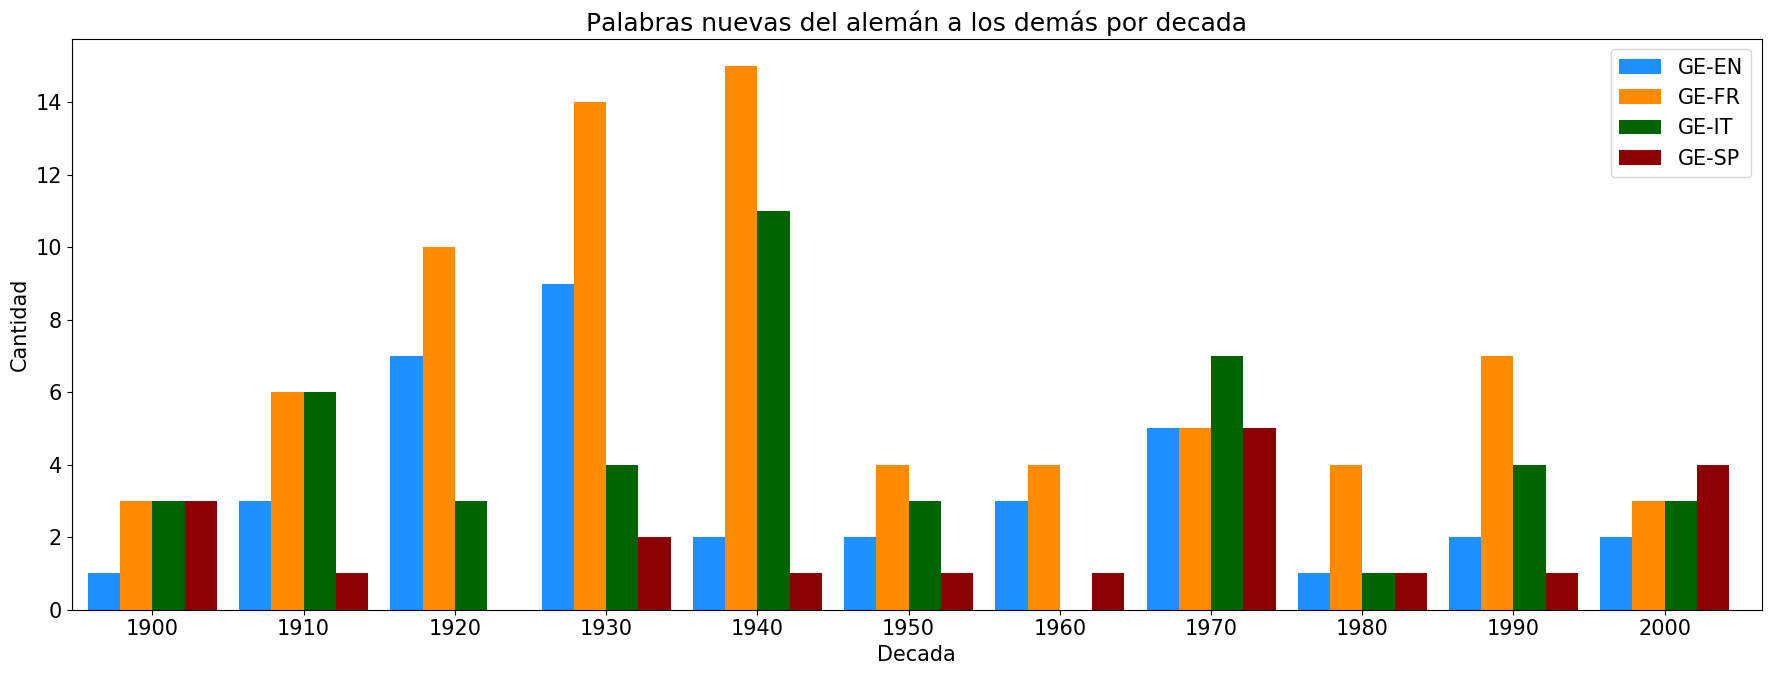
\includegraphics[width=14cm, height=7cm]{Cap_3/ICD_a_GE.png}
				\label{fig.ICD_a_GE}}
		\end{subfigure}
		
		\caption{Palabras nuevas del alemán en los demás.}
		\label{fig.IC_GE}
	\end{center}
\end{figure} % }}}

El principal idioma donde emigraron las palabras del alemán, fue el francés con
casi 70 préstamos, siendo siete veces más que en español, el idioma con menor
cantidad. Destaca el italiano como el segundo con más términos a pesar de que
el inglés proviene de la misma familia de lenguas germánicas.  Campos como el
desarrollo científico, la filosofía  y la política donde los germanoparlantes
tuvieron papeles destacados en el siglo pasado ha hecho posible que las demás
lenguas se impregnan del alemán, y que continuaron usándolos tras la primera
aparición


\subsubsection*{Alemán-Inglés}% {{{

Como en la relación en sentido inverso, en los años posteriores a la segunda guerra mundial,  fueron donde mayores relaciones de palabras se encontraron  \textit{Lenin} (1931), \textit{Hitler} (1934) y \textit{reich} (1939) forman parte  de este contexto histórico.  Otras palabras relevantes son \textit{Marx} (1934) y \textit{Freud}, apellidos de dos personaje sy autores destacados en la filosofía y psicología. 


% }}}
\subsubsection*{Alemán-Francés}% {{{

Como se comento de la grafica por siglo, el francés ha recibido más palabras del alemán que cualquier otro. A pesar de que la mayor cantidad de aportes se dio en la primera mitad de siglo, las relaciones que se encontraron han sido a lo largo de todo el periodo y en diferentes áreas. 

Destaca la década de 1940, con palabras como \textit{regierung},  \textit{deutschen},\textit{minister} y  \textit{bestimmungen}(traducciones de gobierno, alemán, ministro y reglamentos) todas apareciendo en 1944;  si se añaden palabras en años previos como \textit{Hitler} (1933), \textit{kaiser} (1915) y \textit{reich} (1921), son conceptos que muestran parte de la historia del alemán en las guerras. 

El objetivo no es solo identificar sucesos de carácter militar en esta dirección de los préstamos, el identificar un nombre o apellido facilita encontrar las relaciones con un ámbito,  además de Hitler se encontraron los siguientes apellidos:  \textit{Nietzsche} (1905),  \textit{Marx} (1923), \textit{Heidegger} (1987),  \textit{Mozart} (1956), \textit{Freud} (1965) y \textit{Engels} (1970), enlazados a la filosofía, la música y la medicina,  además todos ellos de personajes nacidos en países germanohablantes.


% }}}
\subsubsection*{Alemán-Italiano}% {{{

La proximidad geográfica de Italia con países con lengua oficial en el alemán, hace posible la entrada de palabras, algunas no tan comunes.  Los apellidos de los personajes mencionados anteriormente, también se encuentran en el lenguaje italiano, apareciendo en años próximos a los ya citados.  

El único apellido que se asentó exclusivamente en el  italiano fue \textit{Berchtold} en 1943, aludiendo a Leopold Berchtold ministro de exteriores del Imperio Austro-Húngaro de 1912 a 1915, cuyo fallecimiento ocurrió en 1942.  Se hablo de la proximidad geográfica, ya que este puede ser un factor (ademas del contexto histórico) que detone las migraciones de palabras, la proximidad de Italia con el imperio austro-húngaro puede inferir en la existencia de  palabras que migren entre  dos idiomas y sólo entre ellos. 

  
% }}}
\subsubsection*{Alemán-Español}% {{{

Las palabras que van en este sentido,  presentaron años (o una décadas)  con pocas migraciones o sin alguna, el incremento de palabras se dio posterior a 1950 donde los años sin intercambio disminuyeron.  \textit{Marx} (1932), \textit{kaiser} (1938), \textit{Hitler} (1940), \textit{Lenin} (1970), \textit{Hegel} (1971),  \textit{Nietzsche} (2000) y \textit{Freud} (2002) son parte de los términos que llegaron al español,  sin embargo, es peculiar que las dos últimas hayan aparecido en el español muchos años después que en los demás idiomas, por ejemplo en el francés,  Nietzsche apareció 1905 y Freud en 1965. El letargo de años puede ser una característica del tiempo que les lleva  a las  palabras del alemán pasar hacia el español, al adaptarse a una lengua de una familia distinta y donde históricamente no ha existido un evento conjunto entre países. 



% }}}
% }}}
\subsection{Italiano}% {{{

\begin{figure} % {{{
	\begin{center}
		\begin{subfigure}
			[Italiano por siglo.]{
				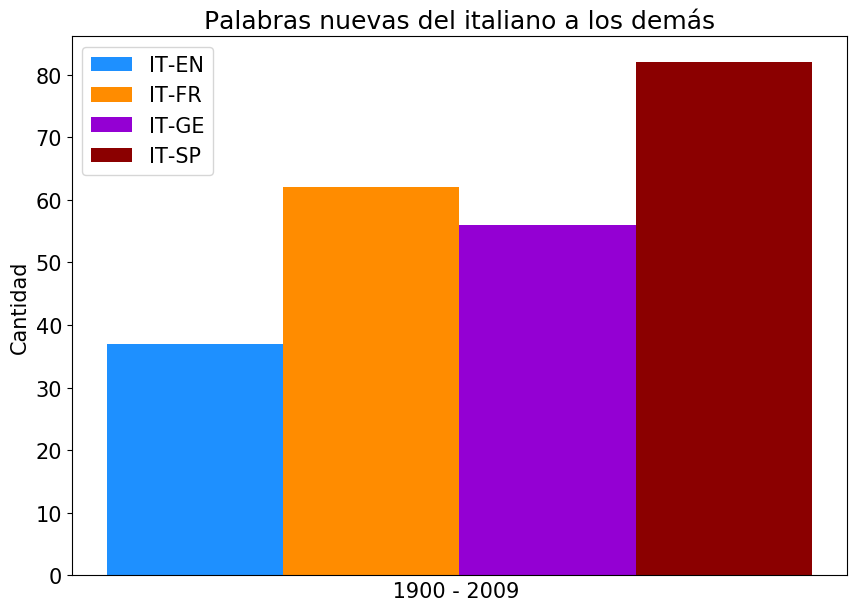
\includegraphics[scale=.4]{Cap_3/ICS_a_IT.png}
				\label{fig.ICS_a_IT}}
		\end{subfigure}
		
		\vspace{0.5cm}
		
		\begin{subfigure}
			[Italiano por década.]{
				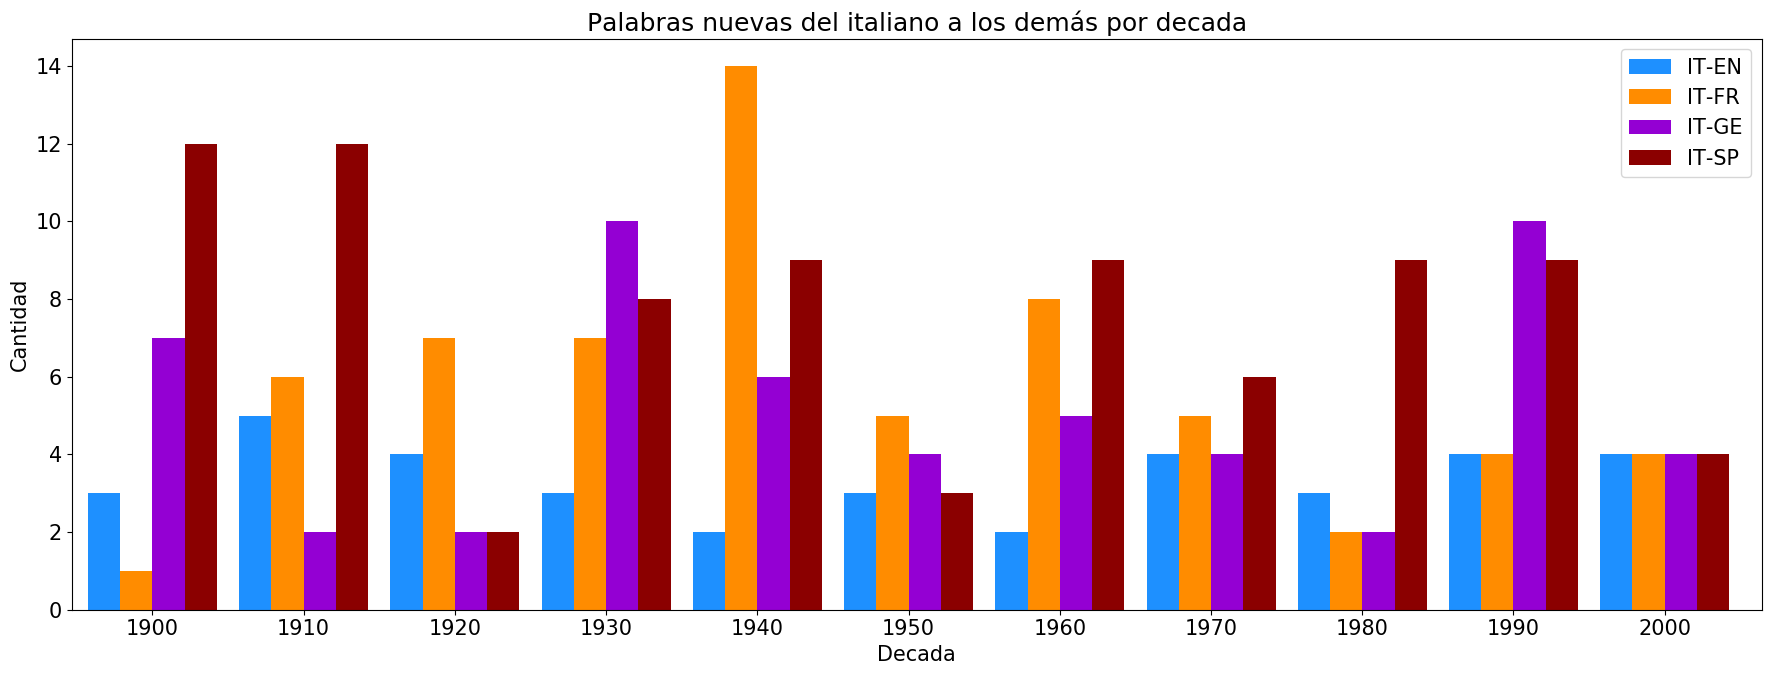
\includegraphics[width=14cm, height=7cm]{Cap_3/ICD_a_IT.png}
				\label{fig.ICD_a_IT}}
		\end{subfigure}
		
		\caption{Palabras nuevas del italiano en los demás.}
		\label{fig.IC_IT}
	\end{center}
\end{figure} % }}}


Por ser lenguajes parecidos fonética y etimológicamente al provenir de la misma
raíz grecolatina,  el español ha adoptado la mayor cantidad de palabras
provenientes del italiano,  seguido del francés otra lengua romance.  

\subsubsection*{Italiano-Inglés}% {{{

A pesar de que en cada década existen términos nuevos en el inglés, solo ha sido posible asociar \textit{mussolini} (1935) al político y militar Benito Mussolini, tal vez el personaje italiano más relevante para la historia en el siglo XX 

% }}}
\subsubsection*{Italiano-Francés}% {{{



En las migraciones sólo se asoció \textit{Mussolini} (1935), la cual ya se había mencionado en las migraciones del italiano al inglés, tras revisar las listas de migraciones con origen italiano  a los demás idiomas, Mussolini siempre se encuentra en todas las migraciones y en el mismo año ratificando la importancia de este término en la historia. 

Aunque en 1940 migraron la mayor cantidad de préstamos, ninguno de ellos ha tenido contexto con los sucesos de esa época. 

% }}}
\subsubsection*{Italiano-Alemán}% {{{

En esta dirección de las palabras del italiano, si fue posible relacionarlas con el contexto bélico,  \textit{regime} (1938), \textit{panzer} (1941), \textit{duce} (1942),  traducciones de régimen, blindado y líder, además de \textit{Mussolini} (1935). 



% }}}
\subsubsection*{Italiano-Español}% {{{

En el español, las tendencias no fueron sólo hacia la guerra, también a idelogías políticas como \textit{socialista} (1914), \textit{comunista} (1932), \textit{capitalismo} (1935), \textit{fascismo} (1937),  \textit{marxismo} (1963) y \textit{terrorismo} (1986). 



% }}}
% }}}
\subsection{Español}% {{{

\begin{figure} % {{{
	\begin{center}
		\begin{subfigure}
			[Español por siglo.]{
				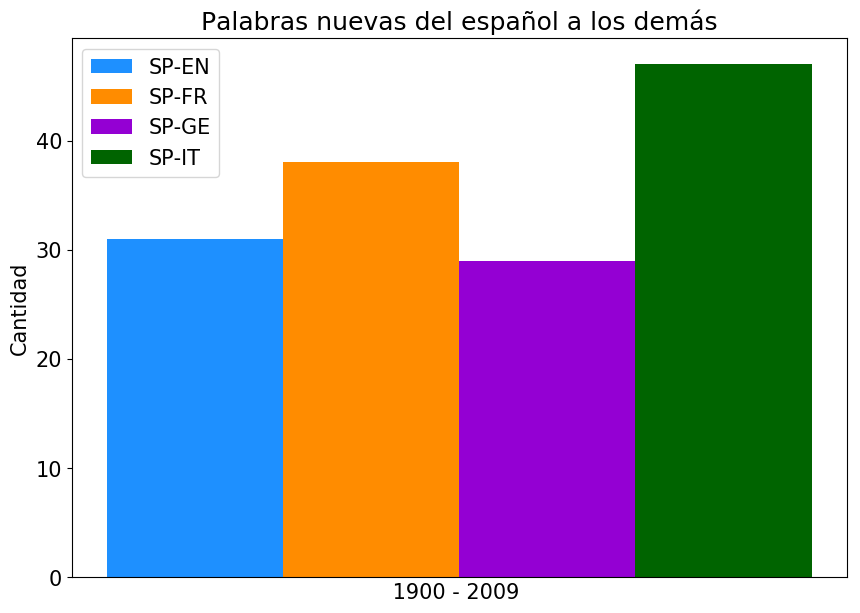
\includegraphics[scale=.4]{Cap_3/ICS_a_SP.png}
				\label{fig.ICS_a_SP}}
		\end{subfigure}
		
		\vspace{0.5cm}
		
		\begin{subfigure}
			[Español por década.]{
				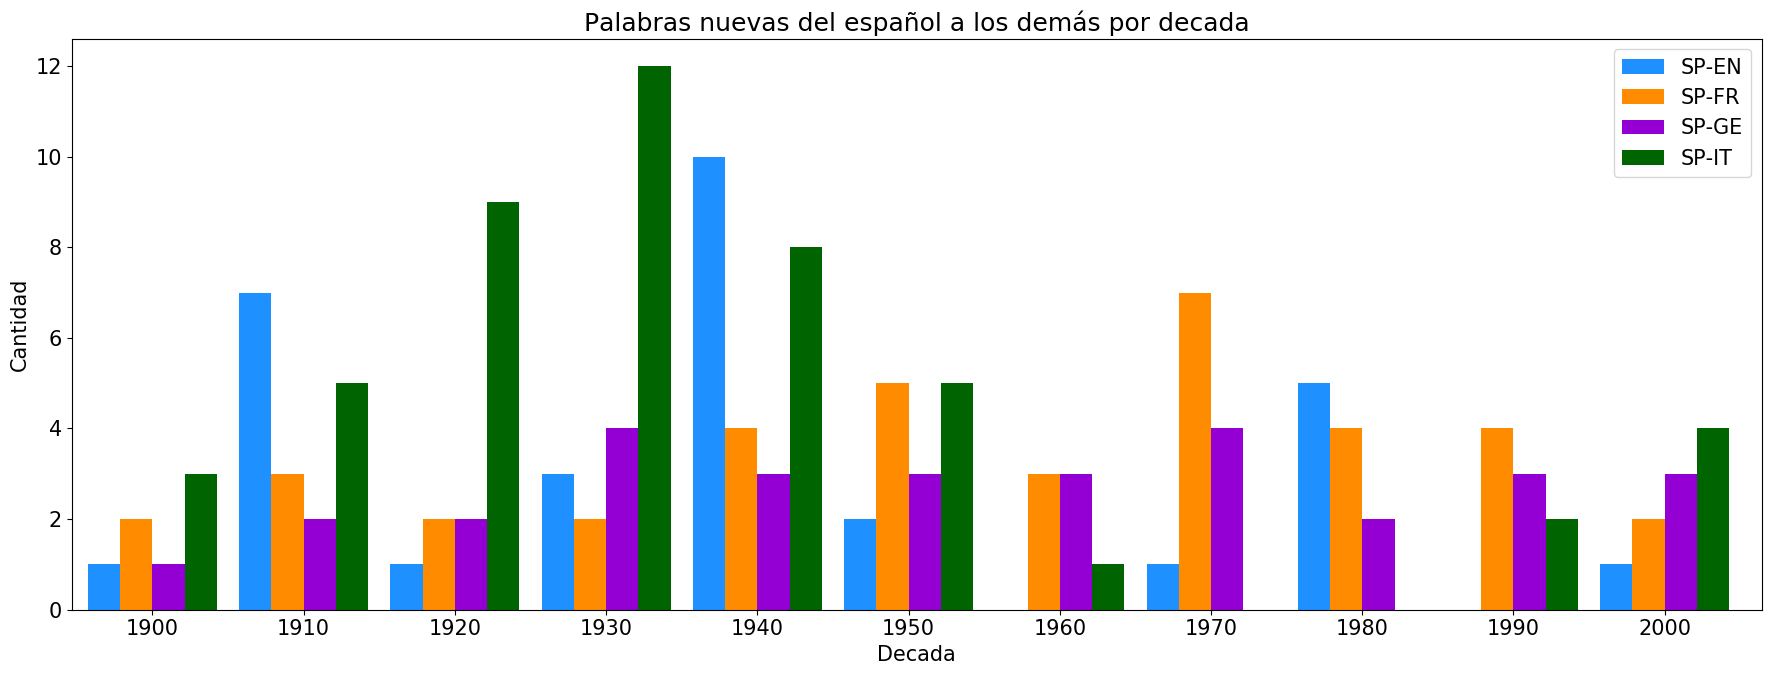
\includegraphics[width=14cm, height=7cm]{Cap_3/ICD_a_SP.png}
				\label{fig.ICD_a_SP}}
		\end{subfigure}
		
		\caption{Palabras nuevas del español en los demás.}
		\label{fig.IC_SP}
	\end{center}
\end{figure} % }}}

Entre todas las combinaciones de idioma origen e idioma receptor,  la relación
entre el español y el italiano, es la única reciproca, donde  el italiano ahora
es el que más palabras recibió del español (anteriormente que el idioma que mas
presencia tuvo en el español fue el italiano).  Nuevamente la otra lengua
romance, el francés es la segunda que mas términos adopto,  mientras que las
germánicas las de menor impacto.  La composición de las etimologías de un
idioma son un factor para que algún otro se adapte en él, es mas sencillo que
existan migraciones entre lenguajes de la misma familia. 

\subsubsection*{Español-Inglés}% {{{

Resalta que hay décadas donde el aporte al inglés es mínimo (o no existe). Contrario a la tendencia en las anteriores migraciones donde la guerra era una constante para que se diese el flujo de palabras, en este sentido se encontraron términos médicos en el año de 1943 (la decadas mas prolifera del español en el inglés) aparecieron las palabras \textit{virus} y \textit{anemia}, años antes en 1934 George Richards Minot, Parry Murphy y George Hoiyt Whipple, habían recibido el premio nobel de medicina por su descubrimiento de la terapia de hígado para el tratamiento de anemias.   

Probablemente las palabras virus y anemia ya existían en el inglés años antes de 1943,  pero sólo hasta este año tuvieron la importancia para estar dentro de las cinco mil mas utilizadas. Con este ejemplo, se trata se ver que hay eventos (como un premio internacional) que retoman palabras cuo periodo de uso  ha disminuido y las vuelve a impulsar para distribuirse en los demás idiomas.   No siempre serán las palabras mas recientes en el origen las que realicen las migraciones. 

% }}}
\subsubsection*{Español-Francés}% {{{

El primer préstamo que resultó importante del español hacia el francés es \textit{Panamá} (1913), su trascendencia se liga al año de inauguración del canal de Panamá en 1914, siendo una obra importante para el comercio de la época al conectar los océanos pacífico y atlántico, además el primer gobierno que impulsó económicamente la construcción del canal fue el francés,  aunque su conclusión y administración pasó a los Estados Unidos.  




% }}}
\subsubsection*{Español-Alemán}% {{{


La investigación hecha para ligar muestran nuevamente términos médicos, la palabra \textit{lepra} (1901) fue globalmente importante a partir de 1874,  ya que en ese año el científico noruego Gerhard Armauer Hansen descubrió el bacilo de Hansen Mycobacterium Leprae \cite{lepra} que origina la enfermedad. Por el carácter médico de la palabra es probable que se hiciera más investigación sobre la enfermedad en diferentes idiomas, en este caso el alemán.

Como en las migraciones hacia el ingles, son términos que vuelven a ser importantes,  y esto les permite migrar a otros idiomas. 


% }}}
\subsubsection*{Español-Italiano}% {{{

Los términos médicos han sido una constante en las migraciones del español,en el italiano se encontraron \textit{virus} (1922), \textit{colesterina} (1928),  \textit{sintomatología} (1931), \textit{anestesia} (1932), \textit{vitamina} (1935), \textit{anemia} (1936), \textit{metabolismo} (1936) y \textit{gástrica} (1936)  y \textit{endovenosa} (1937).  

El aparecer estas palabras en el español (dentro de las cinco mil más usadas)antes que en los demás propone que la medicina era un campo importante para los países de habla española, donde posiblemente en los años del conjunto base (1740-1900) se publicaron más libros de medicina en lenguaje español. 





\hfill\break
\hfill\break

% }}}
% }}}
% }}}
\section{Comentarios del método}% {{{


Tras las múltiples combinaciones entre idiomas, se  encontró que el principal
evento que origino las migraciones ha sido la segunda guerra mundial donde
todos los lenguajes recibieron un termino asociado a ella durante el siglo XX.

Se destaca el papel del inglés en las ultimas dos décadas como el idioma común
para transmitir información; además de ser el exportador de palabras en campos
como la tecnología, disciplina que ha hecho posible la fluidez con la que se
mueve a información. El poderío económico ha hecho de países como los Estados
Unidos una fuente de nueva información.

El alemán también ha acaparado las migraciones, se han distinguido dos causas
de la importancia de este idioma tanto como origen como receptor, la primera
por el papel representado en la historia del siglo XX principalmente por
Alemania donde la guerra permitió la comunicación de varias lenguas con el
alemán, incluso después de que estas terminara, así mismo el protagonismo de
personajes germanoparlantes en diferentes áreas ha hecho que el alemán se
expanda incluso en lenguajes que no son de su propia familia lingüística. 

Finalmente entre las tres lenguas romances, aunque no hayan sido tan
protagonistas (no aporten palabras con un contenido afín),  su periodo de
apogeo e influencia hacia los demás no se tiene registrado en este trabajo.
Destacan los conceptos médicos en la lengua española, mostrando la importancia
que tenia la medicina y la cantidad de libros que se publicaban en esta área en
este idioma. 

Entre las principales deficiencias del método, es que aun es ambiguo decir
quien ha influido mas en los otros; por el momento sólo se puede decir la
manera en que se ha reflejado la influencia, cada conjunto de palabras que
migraron de un idioma a otro, tienen relación a algún ámbito, la guerra, la
economía, la tecnología, las ciencias, las artes y la medicina; cada
combinación tendrá mas elementos de alguna de estas áreas.  Se realizara otro
método para cuantificar la influencia de unos sobre otros. 

% }}}


%\include{Capitulo2/marco_teorico}           % ~20 páginas - Poner un contexto a la tesis, hacer referencia a trabajos actuales en el tema
\chapter{Palabras acumuladas}

La búsqueda para cuantificar la influencia que tiene un idioma, ha llevado a contabilizar las palabras que son nuevas en los distintos receptores y a partir de ellas ligar contextos que amplíen la forma de influencia.  Se ha puesto también énfasis en el conjunto de búsqueda, pero  el conjunto base  también tiene información de cuáles palabras han migrado, además  abarca más años (160 entre 1740 y 2009), por lo que su información es más basta en contenido. 

Para no repetir el proceso de contabilizar a los préstamos nuevos,  se propone pensar que en el primer año del conjunto de búsqueda (1900),  el idioma receptor ya contenía cierta cantidad de palabras que provenían de otros orígenes,  de tal manera que ya forman parte de él, es decir estos préstamos “conviven” con las palabras propias del receptor. Es necesario hacer una nueva definición para estos préstamos.   Dados un idioma  origen  \textit{A} y  la lista para un año  de las palabras más comunes en el receptor \textit{B},  se detonan como: 

\begin{description}
	\item[Préstamos acumulados:] Son las palabras con origen \textit{A} que ya habían aparecido en alguna lista de \textit{B}, y para ese año lo volvieron a hacer.  
\end{description}

La diferencia entre los nuevos y los acumulados es que sólo serán nuevos en el primer año de aparición,  posteriormente a él se convierten en acumulados. 


El objetivo de este estudio es ver cómo se comportan todas las palabras que ya han migrado a un receptor, y si hay una tendencia donde su uso sea alterado. 

Continuando con las distinciones, el método del capitulo anterior se enfoca en la cantidad de palabras nuevas, nunca se trato con la frecuencia de las palabras, ahora se utilizará esta propiedad  para llegar a una cuantificación de la influencia. Si se tienen la lista de las cinco mil palabras más usadas  de \textit{B}, y se distinguen aquellas que provienen de un origen \textit{A} que han aparecido con anterioridad, es decir los préstamos acumulados de \textit{A} en \textit{B}, entonces el proceso para cuantificar el uso de \textit{A} en \textit{B} es el siguiente: 

\newpage

\begin{enumerate}
	
	\item En un año determinado del idioma \textit{B}, se sumarán las frecuencias $f_{i}$ de las cinco mil palabras más usadas.  Esta cantidad se llamará \textbf{frecuencia total por año.}
	
	\begin{equation}
	\label{ec.ftot}
	f_{t} = \sum_{i=1}^{5000} f_{i} \,\,\,\,\,\,\,\,\, i = posici\acute{o}n\,\, de \,\,cada \,\,palabra
	\end{equation}
	
	\item Como se conocen las posiciones $j$,  que ocupan los préstamos \textit{A} en la lista de \textit{B}, se procede a sumar sólo las frecuencias asociadas a estas palabras. Esta cantidad será la \textbf{frecuencia de préstamo} $f_{p}$,  siempre será menor que la frecuencia total por año.
	
	\begin{equation}
	\label{ec.fpres}
	f_{p} = \sum_{j} f_{j} \,\,\,\,\,\,\,\,\, j = posici\acute{o}n\,\, de \,\,cada \,\,pr\acute{e}stamo
	\end{equation}
	
	
	\item  Se divide la frecuencia de préstamo entre la frecuencia total por año, esta cantidad se llamará  \textbf{Uso} $U$ y es la porción que representa \textit{A} en \textit{B} en teŕminos de frecuencia, \textit{El uso de A en B}.  Como en un año hay mas palabras propias de B, esta cantidad es muy pequeña, para tener cifras manejables, se tomara un porcentaje al multiplicar el cociente por cien, así la frecuencia de uso es siempre positiva y toma valores entre cero y cien.  

	\begin{equation}
	\label{ec.fuso}
	 U = \frac{f_{p}}{f_{t}} * 100
	\end{equation}
	
	
	Entre más cercana a 100$\%$ sea el \textit{Uso de A en B}, los préstamos de \textit{A} son más relevantes en \textit{B}.

\end{enumerate}

Entonces,  la nueva forma de medir influencia sera mediante el uso. Lo relevante de trabajar con este método es que  en un determinado año o conjunto de años, se puede ver el uso que han tenido los prestamos con diferentes orígenes en un mismo receptor ó el proceso inverso,  observando el uso que ha tenido un origen en los diferentes receptores. 




\newpage

\section{La influencia en 109 años}

Descritas el tipo de palabras a emplear y la forma de trabajar con ellas, el proceso que se siguió para obtener resultados es el siguiente: 

\begin{itemize}
	
	\item Elegidos un  origen \textit{A} y un receptor \textit{B}, se localizaron en el conjunto base los prestamos acumulados de \textit{A} en \textit{B}. Obteniendo una base de las palabras que ya forman parte de \textit{B} al comienzo del conjunto de búsqueda. 
	
	\item Se empleó la ecuación \ref{ec.fuso} en todos los años del conjunto de búsqueda, obteniendo 109 valores.
	
	\item El proceso se repitió para todas las combinaciones de orígenes y receptores.
	
	\item  Tras cada año del conjunto de búsqueda, se elaboraron nuevas listas de los prestamos acumulados, agrupándolos por cada combinación de origen y receptor. 
	
	\item Para observar los datos como una cantidad que varia en el tiempo, se  hicieron tres tipos de graficas con tres tipos de agrupaciones.
	
	\begin{description}
		
		\item[\textit{A} como origen común.] Graficando el uso de \textit{A} en todos los demás idiomas para observar en que idiomas \textit{A} es más empleado. 
		
		\item[\textit{A} como receptor común.] Graficando el uso de los demás en \textit{A}, observando que idioma es mas empleado en \textit{A}.
		
		\item[Alternando \textit{A} y \textit{B}.]  Se graficó de manera conjunta el uso de \textit{A} en \textit{B}, y el de \textit{B} en \textit{A}, observando en cuales momentos uno fue mas empleado que el otro.
		
		%\item Como se esta trabajando en un periodo de ciento nueve años, el uso será mayor o menor en determinadas épocas; para no repetir el proceso anterior de dividir por décadas, se especificara el periodo donde se tuvo el mayor cambio en el uso y los años que se abarcaron.  
		 
		
	\end{description}	

\end{itemize}

Las listas elaboradas se emplearan en los siguientes capítulos, en el anexo 1 se explica la forma de leerlas así como un vinculo para su consulta. 

\subsection*{Presentación de resultados }

Se continuara con la nomenclatura descrita en el capitulo anterior sobre las abreviaciones y los colores a utilizar, en cada grafica se proporciona una leyenda de la combinación de origen y receptor, indicando la primera abreviatura el origen y la segunda el receptor. 

Por cada idioma se presentaran dos graficas,  la primera será tomando al idioma como origen y ver como se utiliza en los demás receptores, la segunda sera al tomarlo como receptor, para observar como ha sido el uso de los demás orígenes en él. 

En el apéndice A se agregaran las graficas de uso entre dos idiomas, estos resultados servirán para complementar las graficas expuestas en esta sección.

Adicionalmente, la siguiente tabla muestra la cantidad de préstamos acumulados encontrados en cada año del conjunto de búsqueda, especificando los dos idiomas donde se buscaron. La idea de la tabla y el método del uso, es observar que el idioma que más palabras aporta a un receptor no es siempre el más utilizado,  sino que el uso depende de los rangos mas bajos ( las frecuencias mas altas). 


\begin{table}[h!]
	\centering
	\begin{tabular}{lcccccc}
		\multicolumn{7}{c}{R E C E P T O R}                                                                                                                                             \\
		\multirow{6}{*}{\begin{tabular}[c]{@{}l@{}}O\\ R\\ \,I\\ G\\ E\\ N\end{tabular}} &             & \textbf{EN} & \textbf{FR} & \textbf{GE} & \textbf{IT} & \textbf{SP} \\
		& \textbf{EN} & -           & 324.43      & 164.33      & 77.5        & 73.61       \\
		& \textbf{FR} & 297.36      & -           & 94.06       & 118.55      & 66.31       \\
		& \textbf{GE} & 63.87       & 48.06       & -           & 34.92       & 16.61       \\
		& \textbf{IT} & 77.82       & 100.62      & 47.9        & -           & 219.45      \\
		& \textbf{SP} & 118.43      & 84.22       & 29.85       & 311.97      & -          
	\end{tabular}
	\caption{Promedio de préstamos acumulados entre pares de idiomas}
	\label{table.PA}
\end{table}



De la tabla se aprecian dos relaciones similares entre la cantidad de palabras, la primera entre el inglés y el francés si se escoge uno de estos dos idiomas como el idioma origen, entonces el otro funge como el receptor donde las palabras del origen son mayoritarias; la misma característica ocurre con el italiano y el español.  Las relación entre el español y el italiano es esperada, al provenir ambas de la familia de las lenguas romances, la composición etimológica de sus vocablos es semejante,  resultando en una mejor adaptación en el idioma receptor.



\newpage

\section{Palabras acumuladas entre los idiomas}

\subsection{Inglés}


\begin{figure}[h!]
	\begin{center}
		\begin{subfigure}
			[El inglés en los demás.]{
				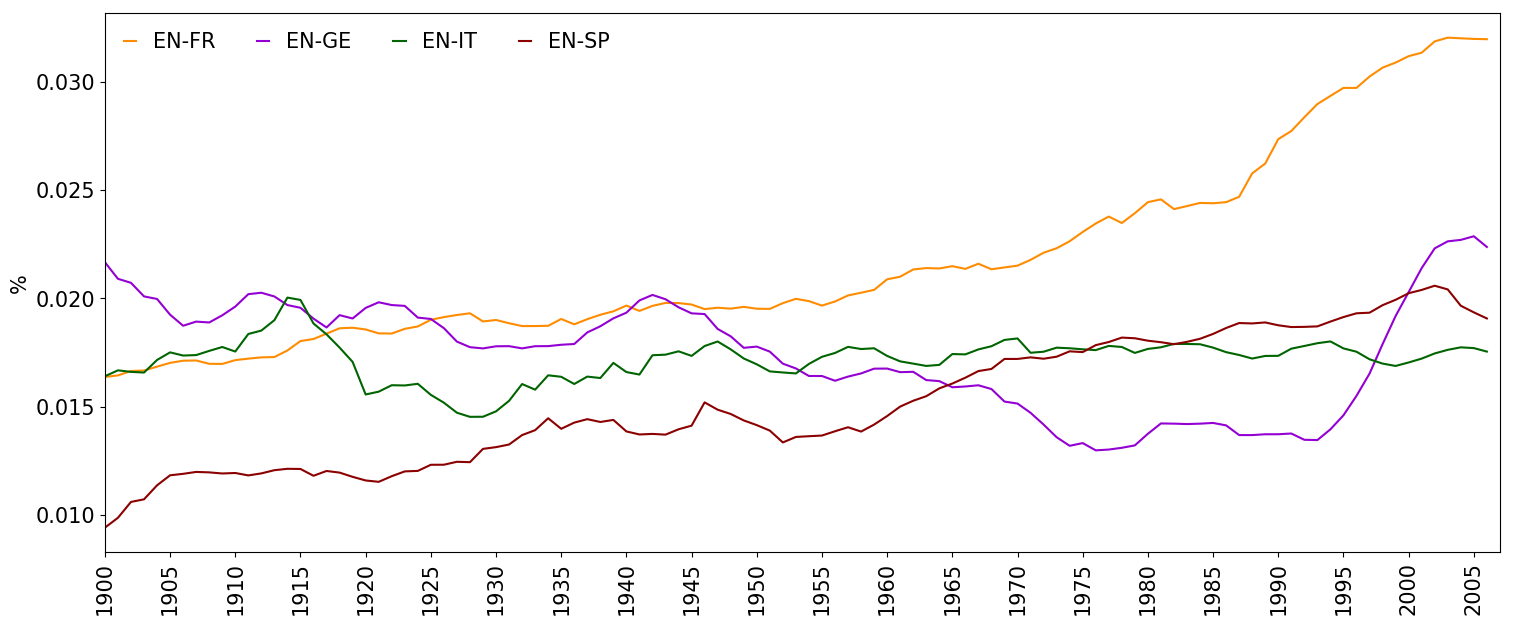
\includegraphics[width=14.5cm, height=7cm]{Cap_4/PF1_S2_EN.png}
				\label{fig.ST_a_EN}}
		\end{subfigure}
		
		\vspace{0.4cm}
		
		\begin{subfigure}
			[Los demás en el inglés.]{
				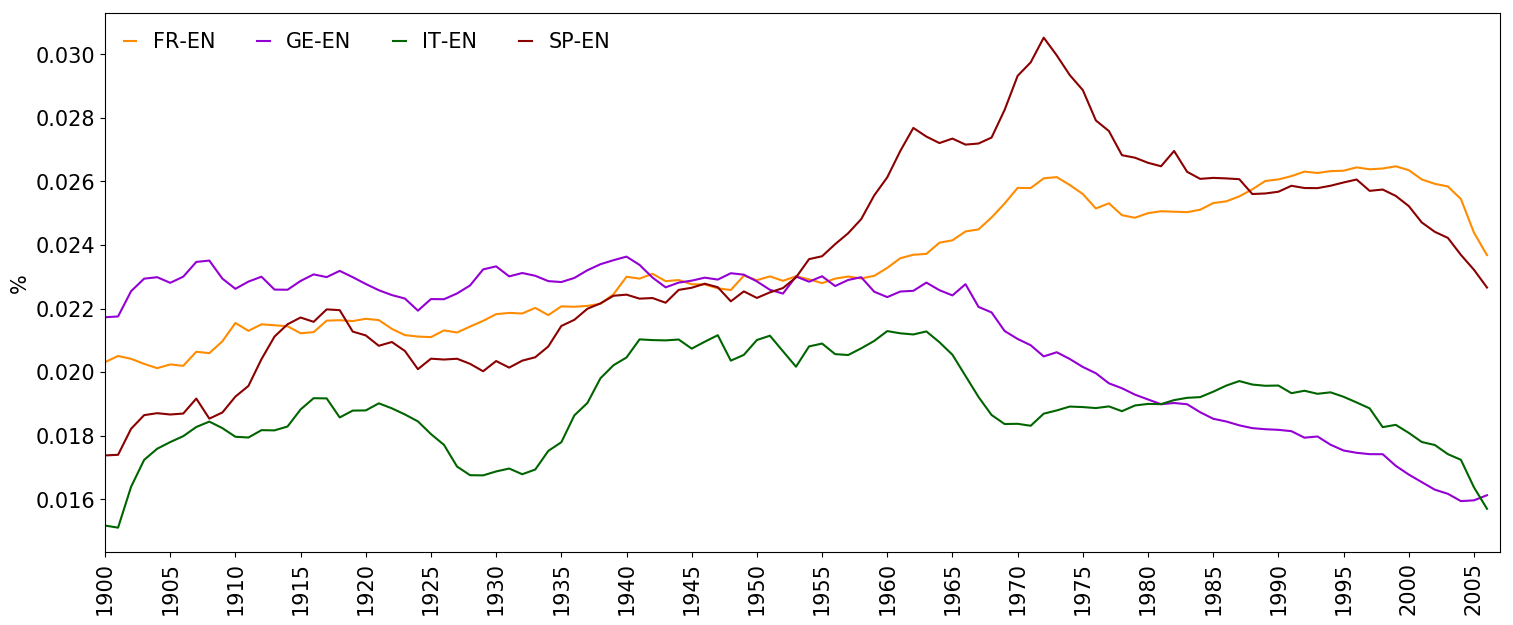
\includegraphics[width=14.5cm, height=7cm]{Cap_4/PF2_S2_EN.png}
				\label{fig.ST_b_EN}}
		\end{subfigure}
		
		\caption{Uso para el inglés}
		\label{fig.ST_EN}
	\end{center}
\end{figure}

\begin{figure}[h!]
	\centering
	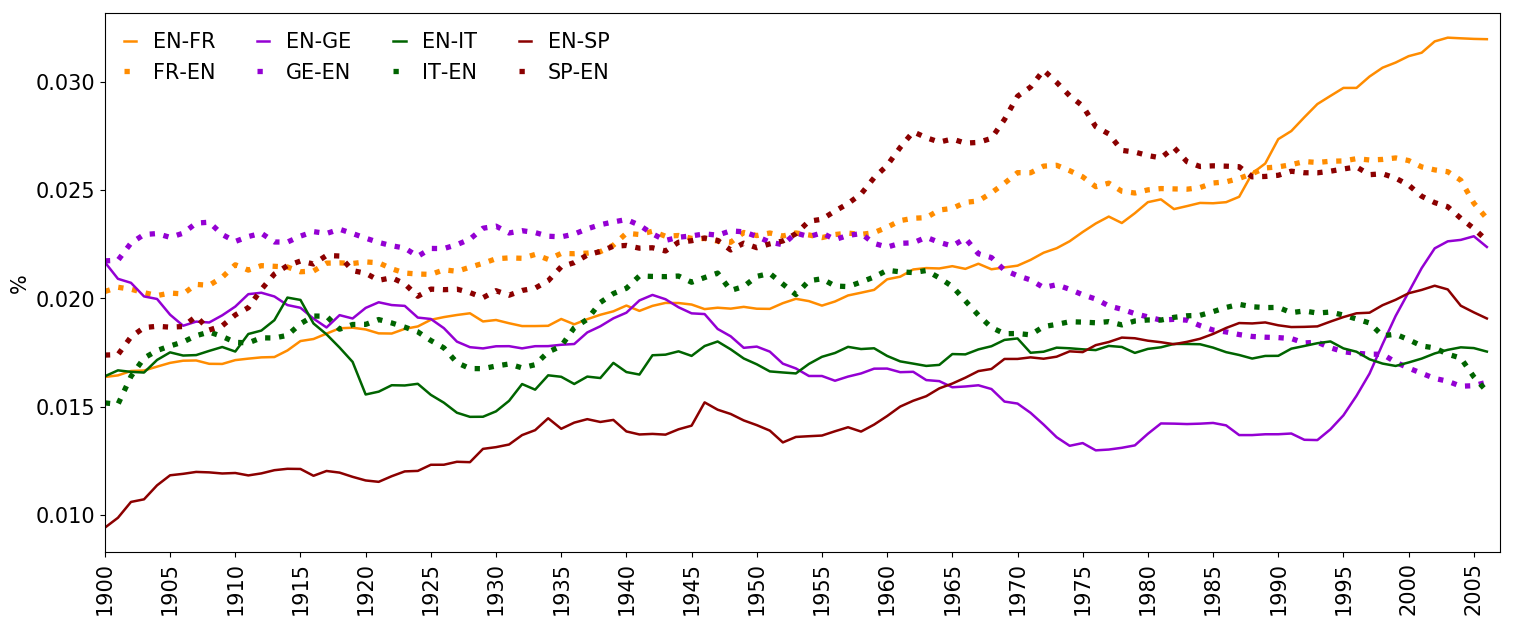
\includegraphics[scale=.38]{Cap_4/UF_EN.png}
	\label{fig.UF_EN}
	\caption{Uso para el inglés.}
	\smallskip
	\small
\end{figure}

\begin{tcolorbox}
	[colback=red!5!white,colframe=red!75!black]
	Me habias comentado que para ahorrar espacioy fuese una grafica más completa, convenia poner las dos graficas anteriores en una sola, yo pienso que al tener una sola grafica se satura la informacion (auqnue cad agrafica tenga diferente color o estilo de linea)
\end{tcolorbox}


Analizando la primera figura, el uso del ingles en los demás ha visto un continuo incremento posterior a 1945 en el francés, el italiano y el español, mientras que en el alemán se da posterior a 1990, año de la finalización del socialismo en Europa con la re-unificación de Alemania, además tras la re-unificación Alemania crece como potencia. 

Del conjunto de prestamos acumulados posteriores a 1945 en los cuatro receptores, el significado común de las palabras son términos políticos, económicos y referentes a la industria como  \textit{capital}, \textit{dollar}, \textit{invesment}, \textit{relations}, \textit{institutions}, \textit{internet} y \textit{software}. El campo semántico de estas palabras, confirma lo encontrado en los prestamos nuevos,  el inglés se ha beneficiado de estas áreas para ser exportado, utilizado y ser el idioma común para transmitir información. 


En los últimos cincuenta años, los idiomas mas comunes en el ingles han sido el español y el francés,  su crecimiento se propaga a partir de  1950, año posterior a la guerra, donde Alemania e Italia fueron derrotados por países de habla inglesa, siendo este un factor que haga decaer al alemán e italiano. El mayor pico  caracterizado por el español,  se relaciona con Aspectos como la proximidad geográfica entre Estados Unidos con Latinoamérica,  el aumento de las migraciones de personas entre ambos costados (siendo mayor el flujo hacia Estados Unidos) surgen como posibilidades del incremento.


\newpage
\subsection{Francés}

\begin{figure}[h!]
	\begin{center}
		\begin{subfigure}
			[El francés en los demás.]{
				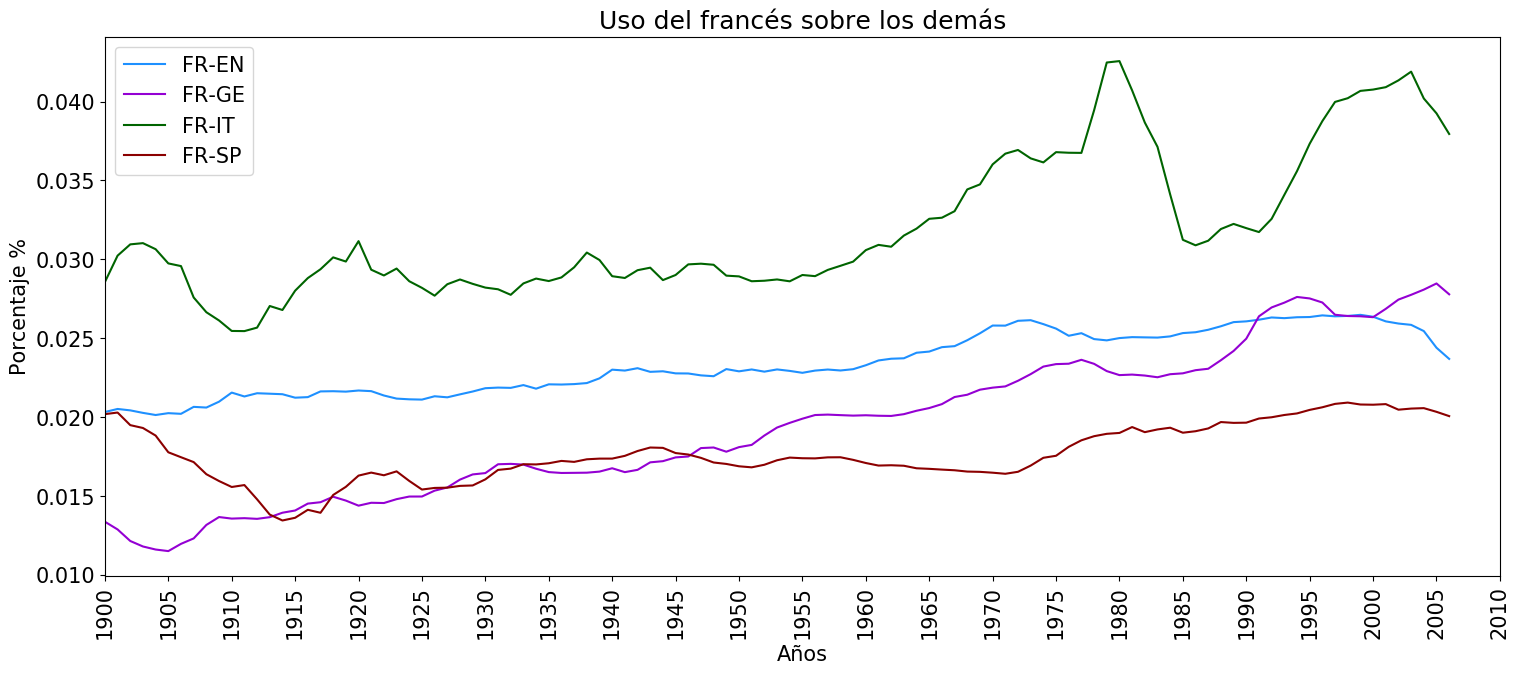
\includegraphics[width=14.5cm, height=7cm]{Cap_4/PF1_S2_FR.png}
				\label{fig.ST_a_FR}}
		\end{subfigure}
		
		\vspace{0.4cm}
		
		\begin{subfigure}
			[Los demás en el francés.]{
				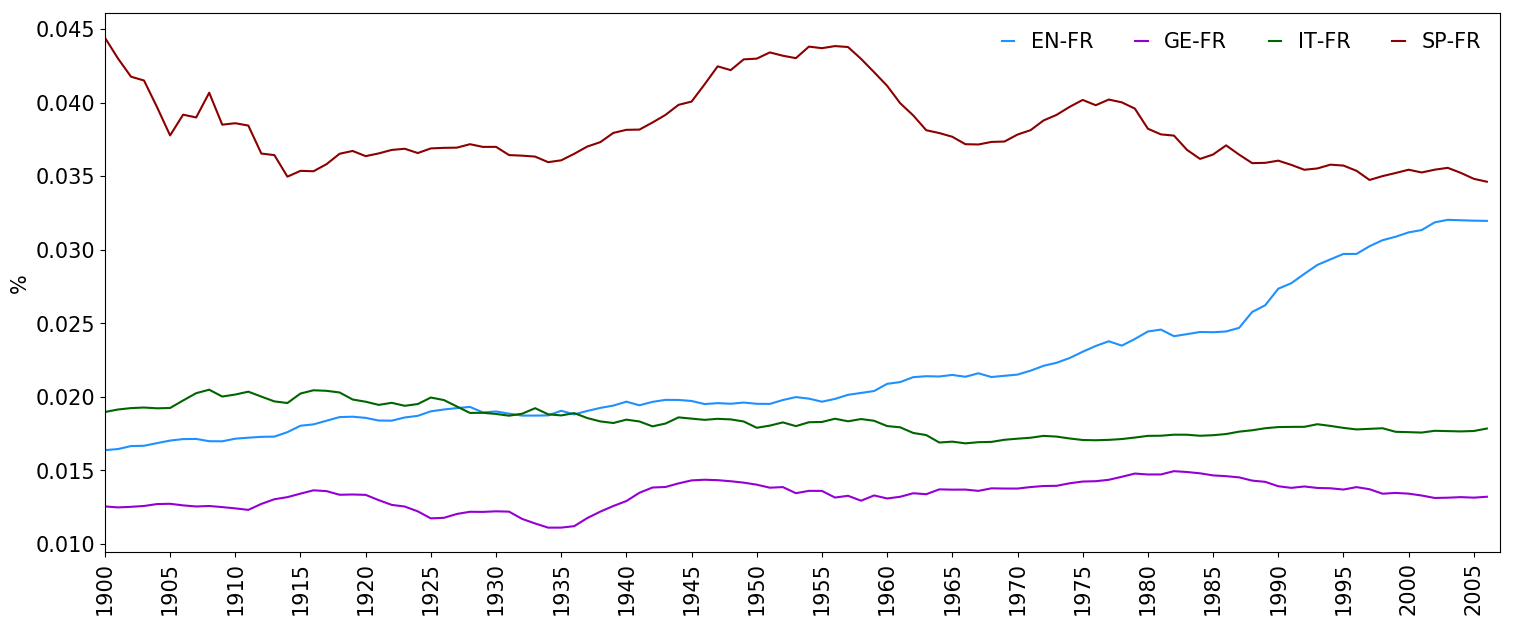
\includegraphics[width=14.5cm, height=7cm]{Cap_4/PF2_S2_FR.png}
				\label{fig.ST_b_FR}}
		\end{subfigure}
		
		\caption{Uso para el francés.}
		\label{fig.ST_FR}
	\end{center}
\end{figure}




A pesar de que el idioma que más préstamos toma del francés es el inglés,  el idioma que más utiliza el francés ha sido el italiano,  aspecto que se mantuvo durante todo el siglo del análisis.  Recapitulando lo comentado en los análisis de los préstamos,  el peso que tuvo la segunda guerra fue un detonante para que el uso entre los idiomas cambiase durante y posterior al conflicto,  en el caso del alemán y del inglés,  el empleo del francés en ellos aumentó tras finalizar el conflicto.  A pesar de que el español y el francés provienen de la familia de las lenguas romances,  el uso del francés en el español se ha mantenido sin mayores alteraciones.



El caso de cómo son utilizados los demás idiomas en el francés,  hay un dominio de las palabras con origen español, seguido por las de origen inglés; aunque el español ha sido el más empleado en el francés,  el inglés a partir de 1940 comienza a ser más frecuentado,  recortando en cada año la diferencia con el español,  siendo en la última parte del estudio  menor al 0.05$\%$, incluso si la base de datos abarcara más años posteriores al 2009, es probable que el uso el inglés pase al español. 



\newpage
\subsection{Alemán}

\begin{figure}[h!]
	\begin{center}
		\begin{subfigure}
			[El alemán en los demás.]{
				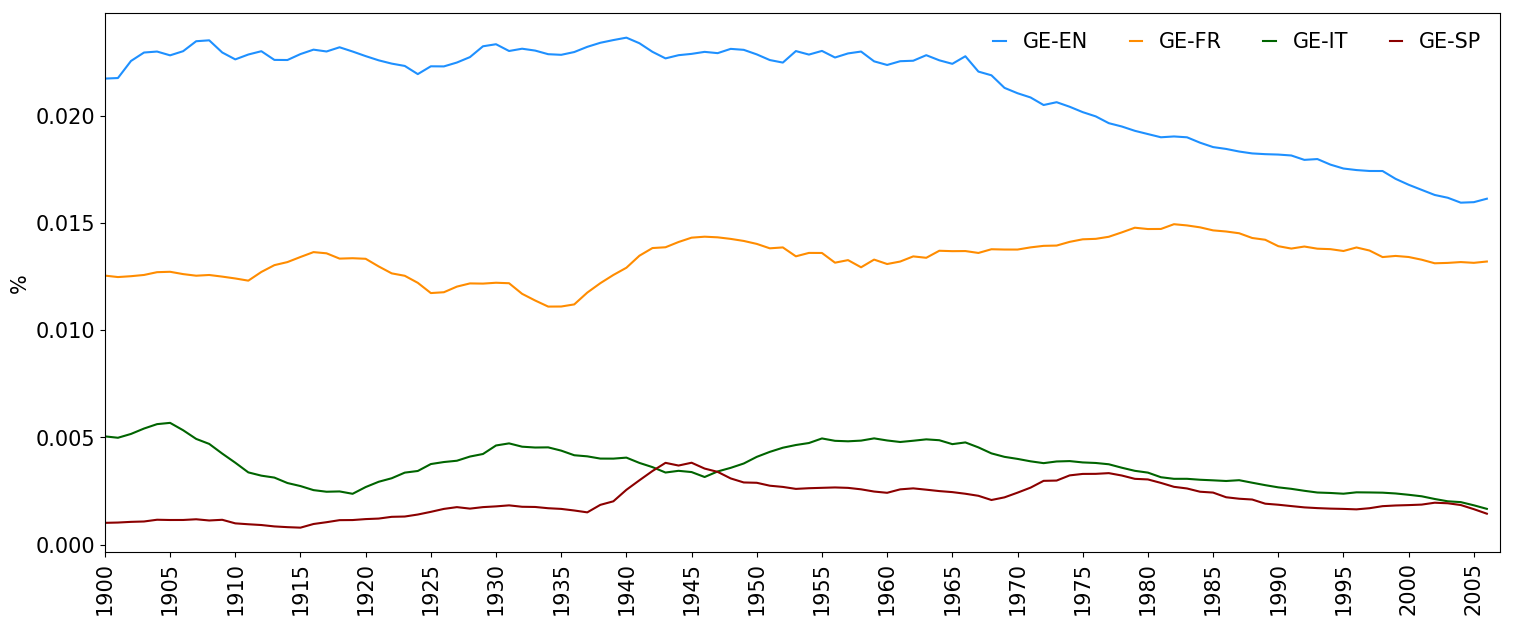
\includegraphics[width=14.5cm, height=7cm]{Cap_4/PF1_S2_GE.png}
				\label{fig.ST_a_GE}}
		\end{subfigure}
		
		\vspace{0.5cm}
		
		\begin{subfigure}
			[Los demás en el alemán.]{
				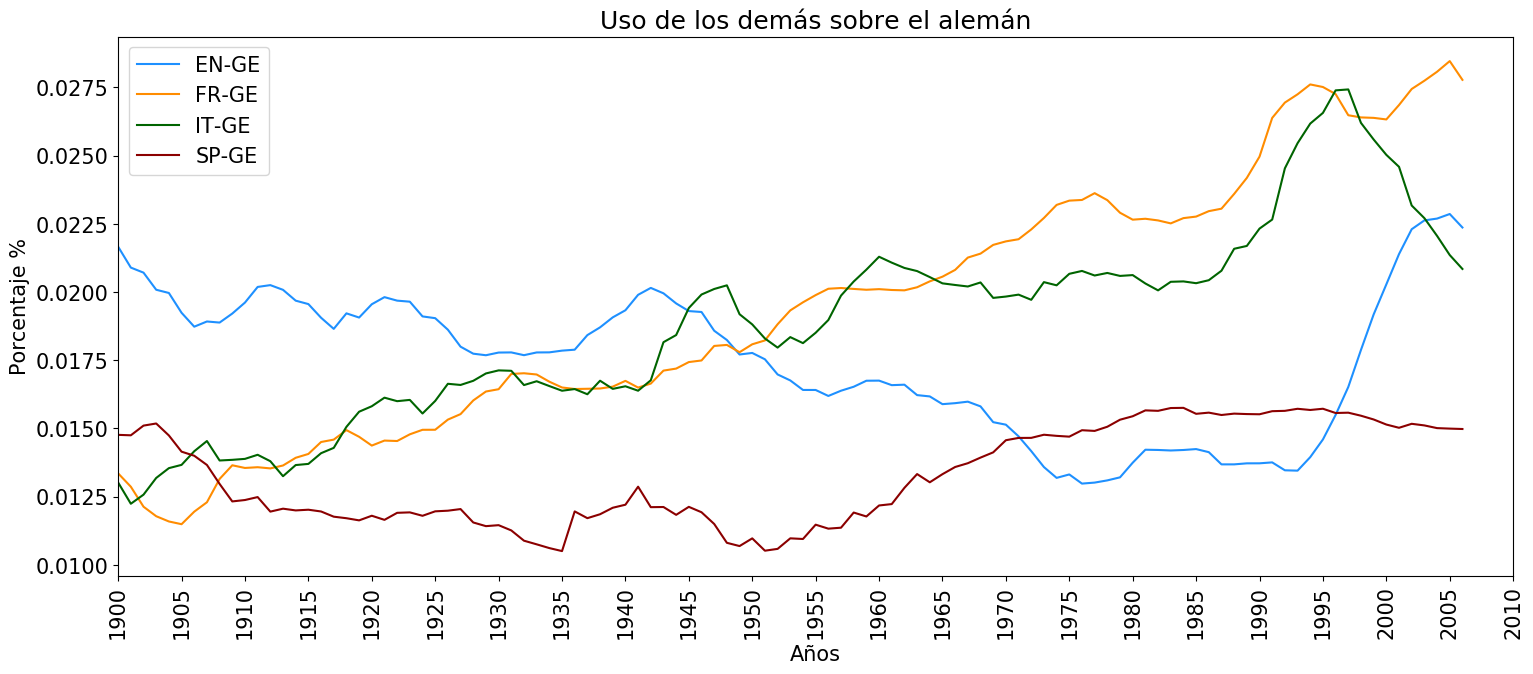
\includegraphics[width=14.5cm, height=7cm]{Cap_4/PF2_S2_GE.png}
				\label{fig.ST_b_GE}}
		\end{subfigure}
		
		\caption{Uso para el alemán.}
		\label{fig.ST_GE}
	\end{center}
\end{figure}



De acuerdo a la tabla \ref{table.PA},  el inglés, el francés, el italiano y el español, son en ese orden idiomas que más préstamos tienen provenientes del alemán, a pesar de que el alemán sea en cada uno el idioma del que menos se componen.  El orden de los idiomas que más emplean el alemán es el mismo que los idiomas que más se componen del alemán, siendo el único caso donde la mayor cantidad es también el mayor uso. Una razón de esta característica es que tanto el alemán como el inglés provienen de la misma familia lingüística, la germánica,  siendo más comunes las palabras entre ellos  que con las lenguas romances.

El sentido de cómo se utilizan los demás idiomas en el alemán, no presenta la característica anterior,   donde se ha alternado entre el inglés, el francés y el italiano el idioma que es más utilizado en el alemán.  El inglés fue el más empleado en la primera mitad del siglo, mientras que posterior a la guerra que ha sido el común detonante para que se altere el uso de un idioma en otro,  francés e italiano rolaron el papel del idioma más común en el alemán. 


\newpage
\subsection{Italiano}

\begin{figure}[h!]
	\begin{center}
		\begin{subfigure}
			[El italiano en los demás.]{
				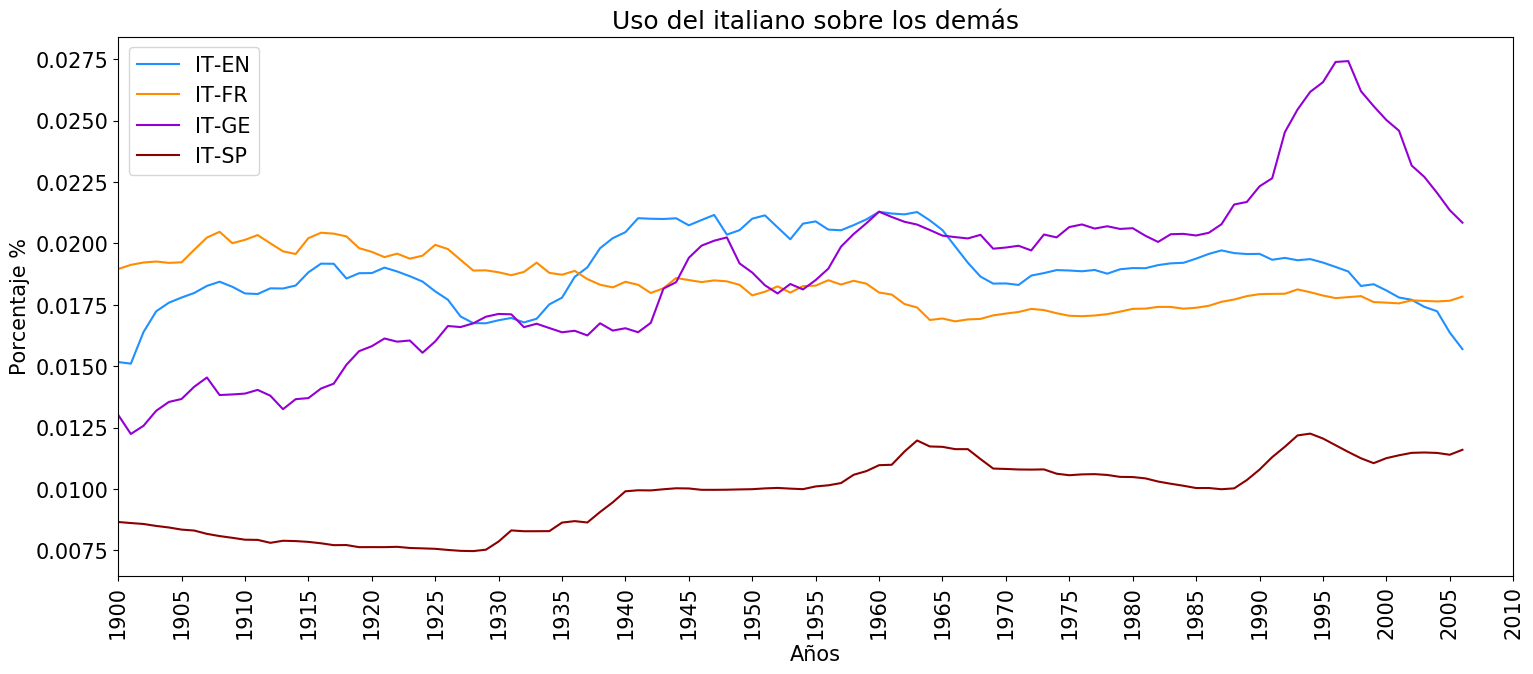
\includegraphics[width=14.5cm, height=7cm]{Cap_4/PF1_S2_IT.png}
				\label{fig.ST_a_IT}}
		\end{subfigure}
		
		\vspace{0.5cm}
		
		\begin{subfigure}
			[Los demás en el italiano.]{
				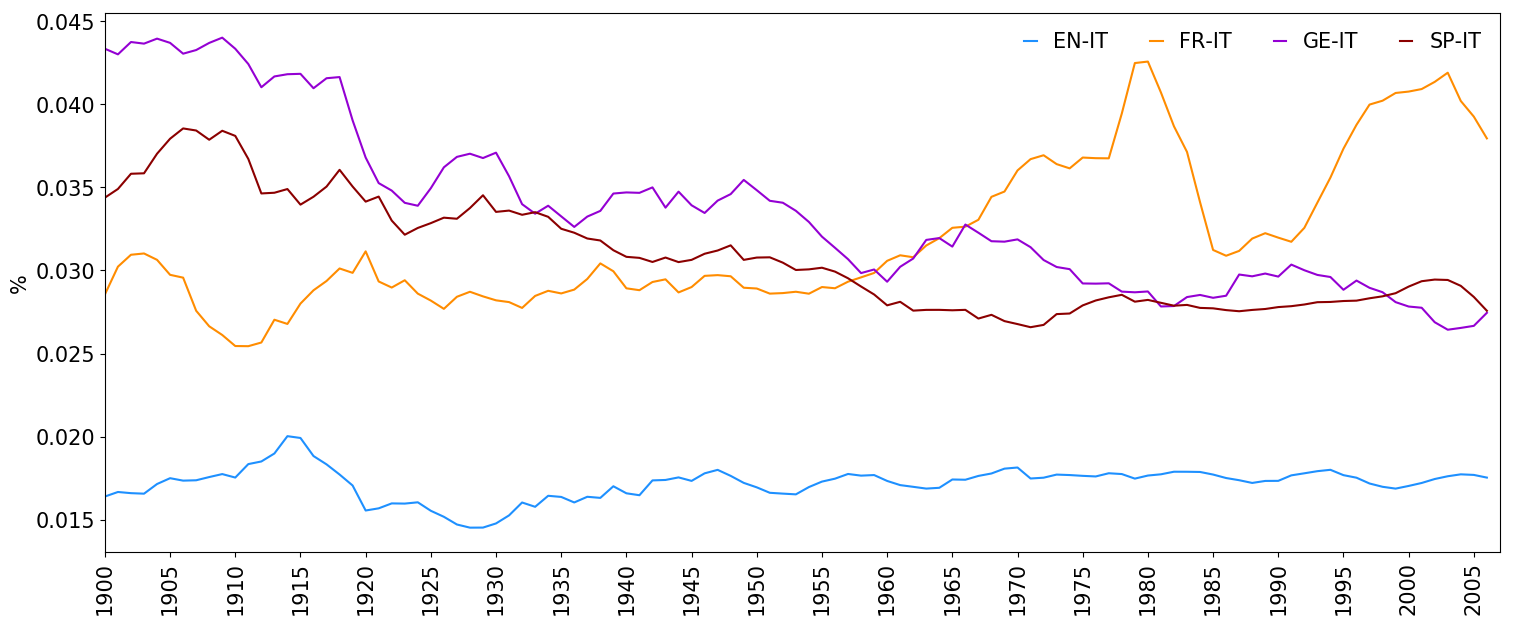
\includegraphics[width=14.5cm, height=7cm]{Cap_4/PF2_S2_IT.png}
				\label{fig.ST_b_IT}}
		\end{subfigure}
		
		\caption{Uso para el italiano.}
		\label{fig.ST_IT}
	\end{center}
\end{figure}

Los idiomas en los que el italiano ha tenido una mayor influencia han sido el inglés, el francés y el alemán pese a que el español es el idioma que más préstamos contiene del  italiano,  circunstancias como la cercanía geográfica entre los países de habla alemán con Italia alude al  mayor uso del italiano en este idioma a partir de  la segunda mitad del siglo,  respecto al inglés,  la intervención de personajes  italianos en la historia y el hecho de que el inglés se compone de palabras de origen grecolatino,  permite que el italiano sea una lengua fuerte en el inglés;  las afirmaciones anteriores se han respaldado en que las palabras de contenido han sido previamente relacionadas  a sucesos donde han intervenido estos países.


La forma de actuar de los demás idiomas en el italiano no es recíproca a la forma en que el italiano interviene en ellos.  El caso del inglés es particular, porque a pesar del impacto que ha manifestado el inglés en los demás idiomas  en los últimos cincuenta años por la globalización,  en el italiano ha sido el único idioma donde no ha sido dominante en algún punto, o donde no ha crecido más que los demás.  El alemán ha sido más importante al comienzo del siglo y decae tras finalizar la segunda guerra mundial, para imponerse el francés como el idioma que más es utilizado en el italiano. 


\newpage
\subsection{Español}

\begin{figure}[h!]
	\begin{center}
		\begin{subfigure}
			[El español en los demás.]{
				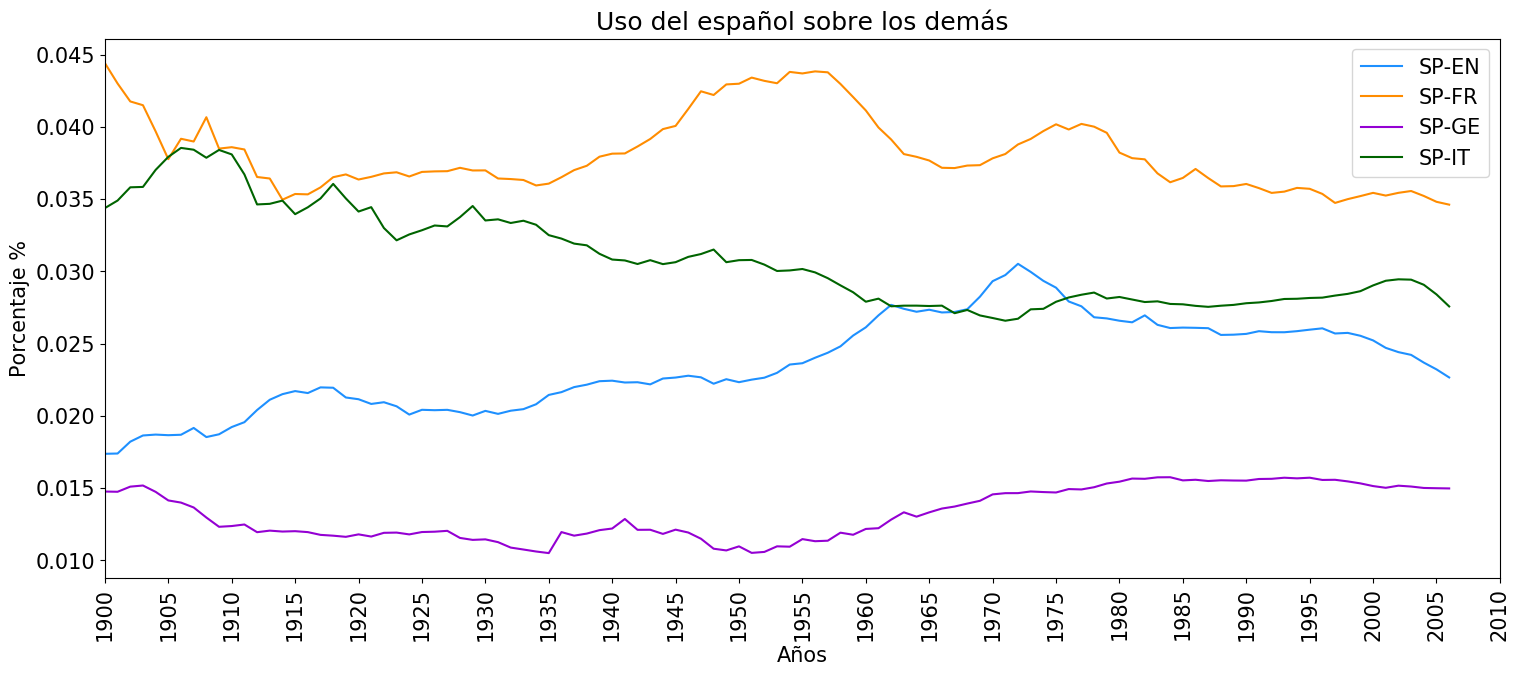
\includegraphics[width=14.5cm, height=7cm]{Cap_4/PF1_S2_SP.png}
				\label{fig.ST_a_SP}}
		\end{subfigure}
		
		\vspace{0.5cm}
		
		\begin{subfigure}
			[Los demás en el español.]{
				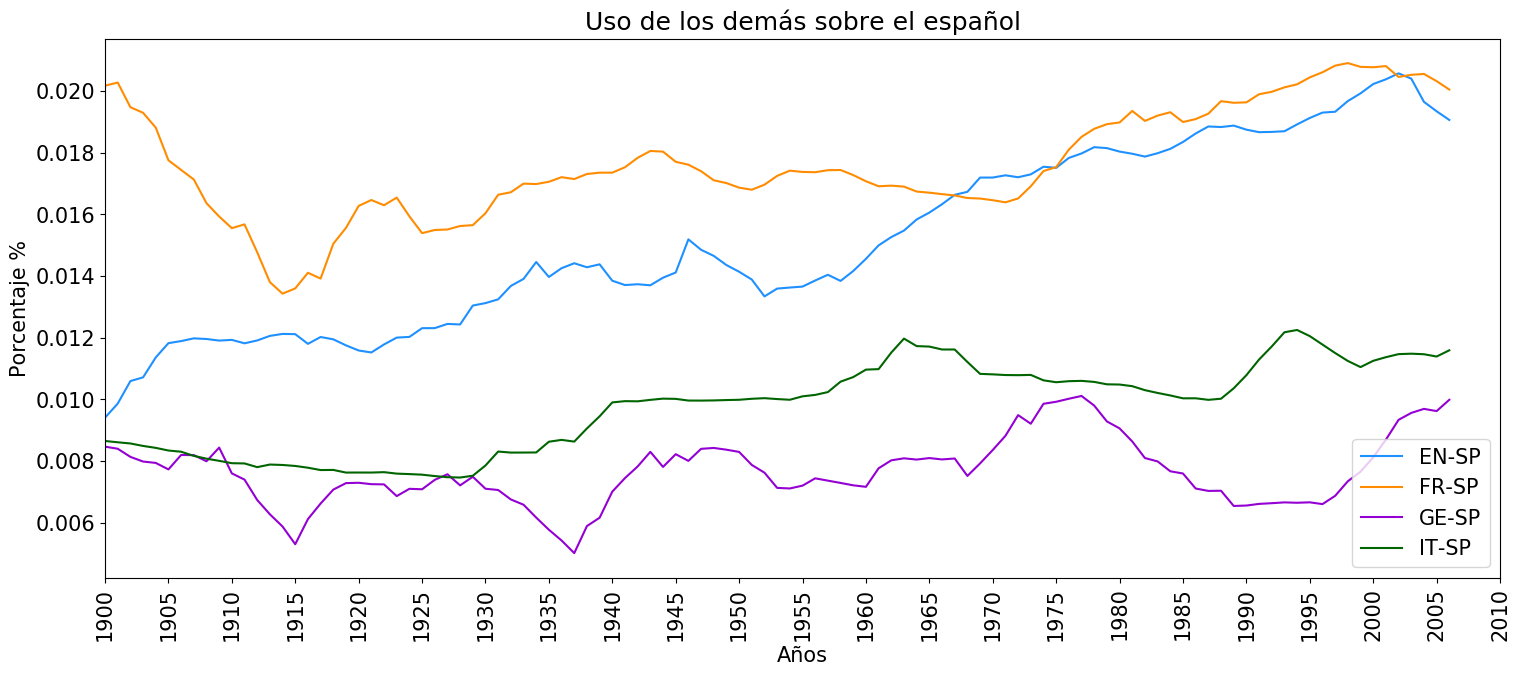
\includegraphics[width=14.5cm, height=7cm]{Cap_4/PF2_S2_SP.png}
				\label{fig.ST_b_SP}}
		\end{subfigure}
		
		\caption{Uso para el español.}
		\label{fig.ST_SP}
	\end{center}
\end{figure}


Entre los gráficos del apéndice 1 de uso entre un determinado idioma y el español, se observó que el español ha sido más influyente en los demás que los demás en él,  siendo el francés el idioma donde el español es más utilizado, a pesar de que la cantidad de préstamos en el italiano es mayor, la causa mas lógica  de esta situación es el provenir ambos de la familia de las lenguas romances. 

Entre la forma en la que se usan los préstamos de los demás idiomas en el español,  en los últimos cincuenta años, la mayor influencia se ve compartida entre las palabras que vienen del francés y  del inglés;  la familia de las lenguas romances y sus similitudes hacen posible que el francés tome relevancia, mientras que la globalización y el crecimiento económico de países de habla inglesa hace relevante al inglés en el español.   Por otro lado,  el italiano y el alemán  no presentan el mismo crecimiento que el francés y el inglés,  por parte del italiano se ha comentado que al ser lengua romance al igual que el español,  el periodo donde los préstamos modificaban el uso del idioma receptor pudiese ser tan antiguo como el surgimiento de los idiomas,  por ello comparten gran cantidad de palabras pero estas no alteran el comportamiento del receptor; mientras que en el caso del alemán la poca relación con el español y el no haber existido un evento que los involucren,  hace que estos idiomas no se hayan mezclado como los demás,  por ejemplo alrededor de 1915 y 1935,  el alemán en el español es casi nulo, a pesar de que en esas fechas se desarrollaron las grandes guerras.


\newpage
\section{Comentarios y complementos del método}


El determinar la influencia entre idiomas a través del uso de los préstamos, ha mostrado primeramente que el idioma que mas cantidad de palabras tiene en otro no siempre es el más utilizado,  radicando el mayor uso en aquel idioma cuyas préstamos tengan menores rangos en la lista de un receptor. 

En todo el siglo XX y la primer década del XXI, el inglés y el alemán han sido los idiomas más cambiantes en los papeles de origen y receptor respectivamente.
El inglés al ser el que más creció en tres idiomas (francés, alemán y español), complementando los resultados del capitulo anterior, al ser el idioma que más palabras nuevas exportó.  El alemán como el receptor donde los diferentes orígenes aumentaron su usó tras la segunda guerra mundial; el uso ha sido semejante a los préstamos nuevos, ha sido el receptor que más recibió. 

Ambos análisis se complementan,  el idioma más influyente ha aportado más palabras nuevas y aquellas que se van acumulando resultan las de mayor incremento en el uso. El idioma más influenciado recibió la mayor cantidad de palabras nuevas y el uso que han tenido los demás ha sido también el del mayor incremento. 

Por el momento sólo es posible describir que originó las variaciones en el uso o en la cantidad de nuevas palabras, no es posible predecir como se comportaran los idiomas en el futuro, ya que la principal característica que  hace fluir a las palabras entre idiomas han sido los eventos, reflejado en que las palabras de su campo semántico  se muevan a diferentes idiomas y continúen apareciendo o desapareciendo tras el suceso. 

Una mejor información de como los eventos alteran a los idiomas se podría extraer si se compararán las características de los prestamos con  datos de los países de alguna habla como lo pueden ser  el crecimiento economizo, el producto interno bruto, la alfabetización, la mortalidad, las migraciones de personas, entre otros.








      % ~20 páginas - Explicar el problema en específico que se va a resolver, la metodología y experimentos/métodos utilizados
\chapter{Omisión de palabras}

Anteriormente se especificó que la base de datos de los préstamos serían únicamente palabras de contenido, y a partir de ellas se realizaron los análisis anteriores.  Al trabajar con las palabras de contenido se están restringiendo a todas las palabras que pueden ser catalogadas como préstamos (algunos artículos o pronombres de un determinado idioma se encuentran en los demás), sin embargo los resultados obtenidos han reflejado contextos históricos en los cuáles explicar las migraciones de palabras, por lo que las restricciones han ayudado a deducciones más claras. 

Por el momento ya no se tratara con la misma regularidad a la interpretación histórica de las migraciones, se centrara las siguientes partes en la forma en que se modifican los resultados al hacer diferentes restricciones en el conjunto de préstamos. 

Si se toman como verdadero al uso de un idioma sobre otro, discutido en capítulo 3,  del conjunto de palabras que conforman en uso de un idioma se propondrán diferentes reglas para restringir al conjunto y observar cómo es que cambian los datos del conjunto reducido por la restricción contra el conjunto original.  

Por ejemplo,  si la regla es omitir las palabras que comiencen con la letra C,  el conjunto original contendrá a todos los préstamos,  el conjunto reducido  no tendrá  préstamos cuya primer letra sea C y el conjunto de las restricciones serán todos los préstamos que empiecen con C. Una vez separados los conjuntos en cada uno se realizó el proceso de  la ecuación \ref{ec.fuso}, para obtener el uso.

Todas las reglas para las omisiones serán eliminando las palabras que comienzan con una determinada letra, en algunos casos se optó por hacer hasta cuatro omisiones con la intención de restringir cada vez más a los conjuntos.  Para una adecuada comparación del uso de un idioma sobre otro, se gráfico de manera continua y  en color negro al conjunto original,  mientras que puntos de dispersión de color rojo al conjunto reducido.


\newpage
\subsection{Inglés}

\begin{figure}[h!]
	\centering
	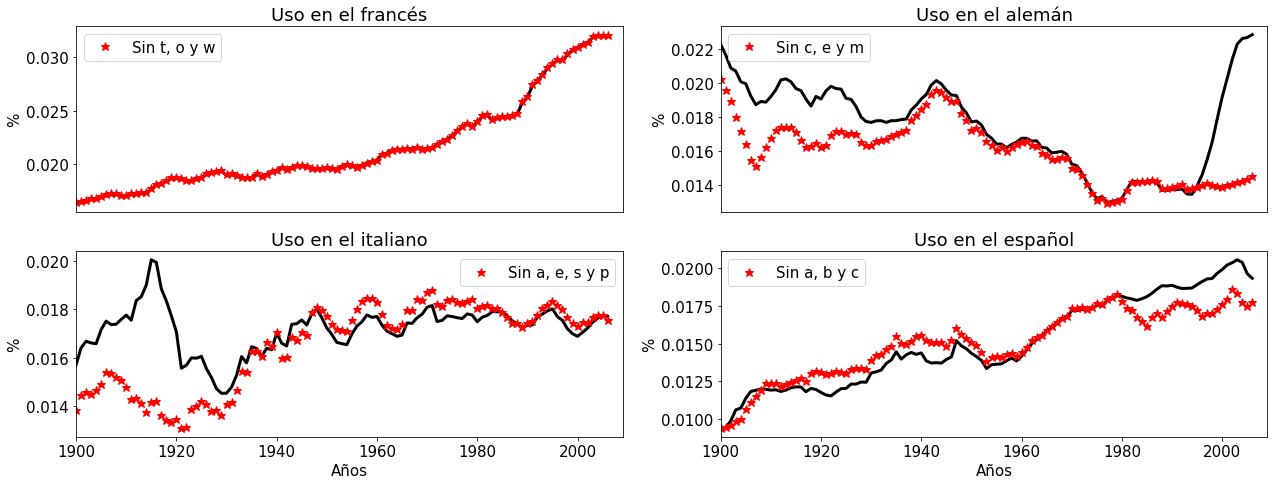
\includegraphics[scale=.375]{Cap_5/OM_EN.png}
	\label{fig.OM_EN}
	\caption{Omisiones del inglés en los demás}
\end{figure}



\newpage
\subsection{Francés}

\begin{figure}[h!]
	\centering
	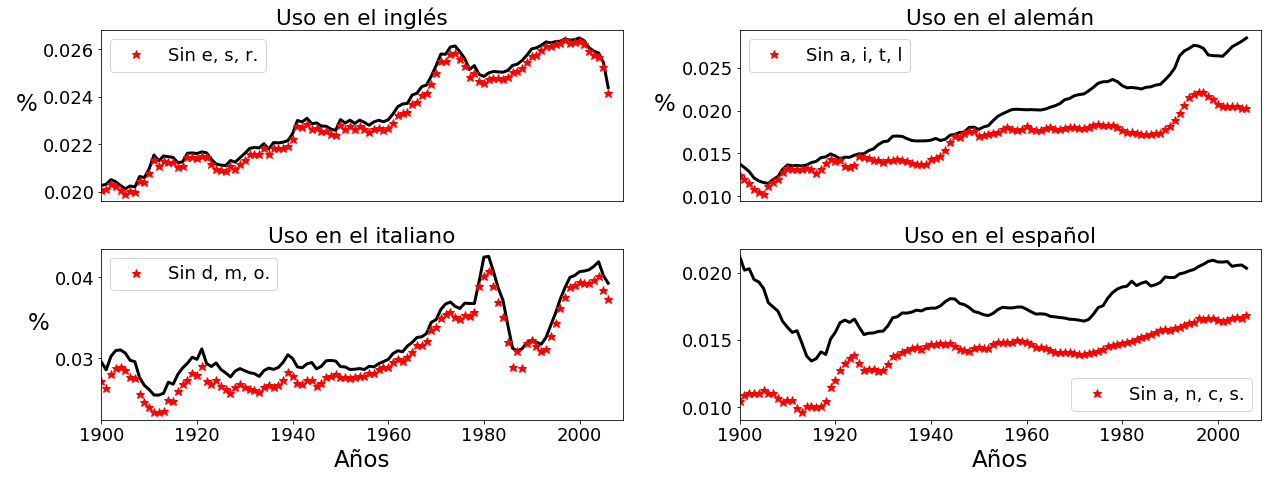
\includegraphics[scale=.375]{Cap_5/OM_FR.png}
	\label{fig.OM_FR}
	\caption{Omisiones del francés en los demás}
\end{figure}


\newpage
\subsection{Alemán}

\begin{figure}[h!]
	\centering
	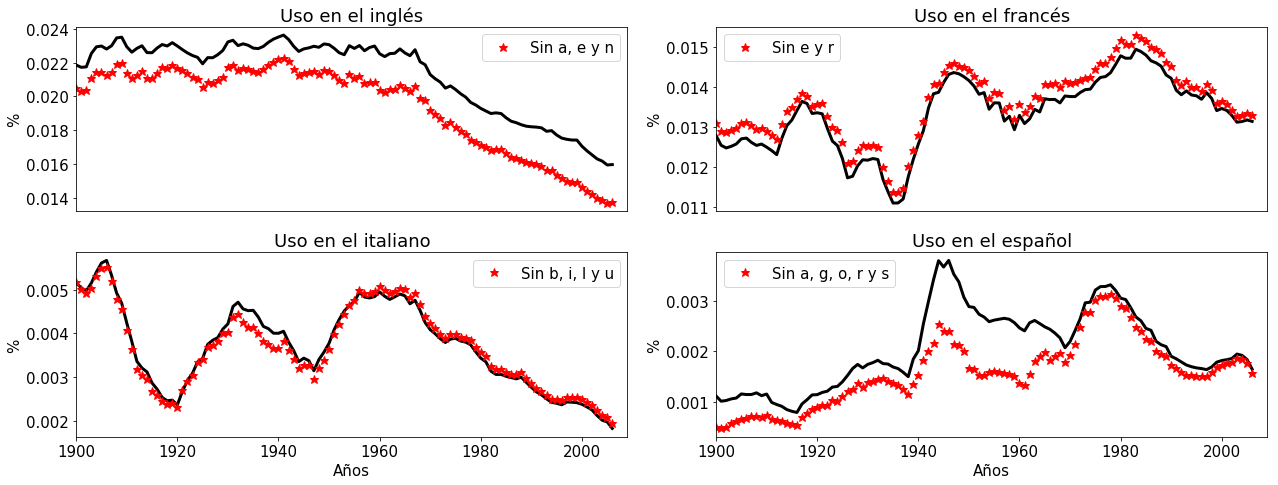
\includegraphics[scale=.375]{Cap_5/OM_GE.png}
	\label{fig.OM_GE}
	\caption{Omisiones del alemán en los demás}
\end{figure}


\newpage
\subsection{Italiano}

\begin{figure}[h!]
	\centering
	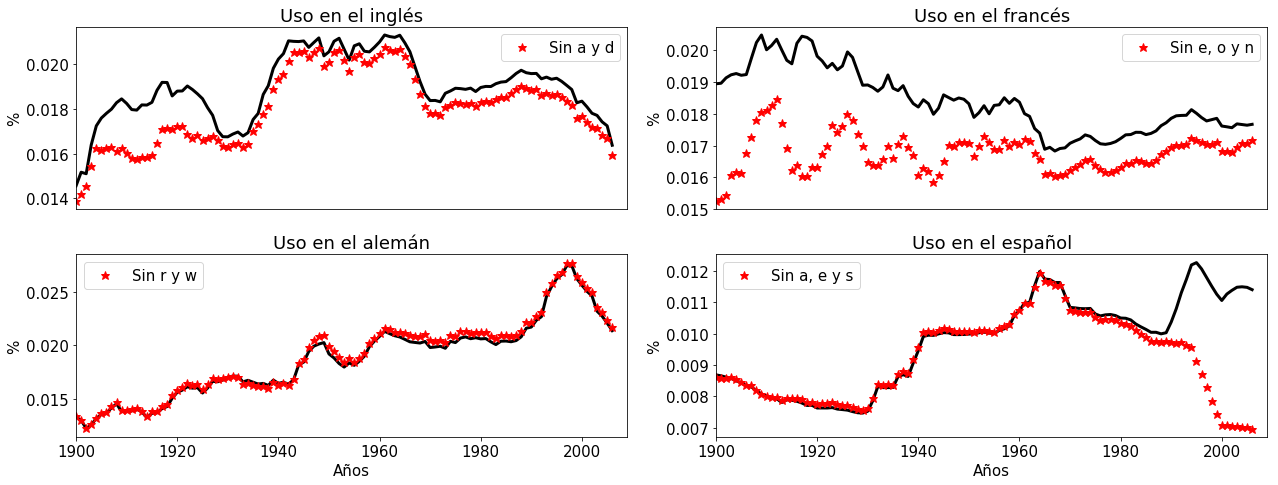
\includegraphics[scale=.375]{Cap_5/OM_IT.png}
	\label{fig.OM_IT}
	\caption{Omisiones del italiano en los demás}
\end{figure}


\newpage
\subsection{Español}

\begin{figure}[h!]
	\centering
	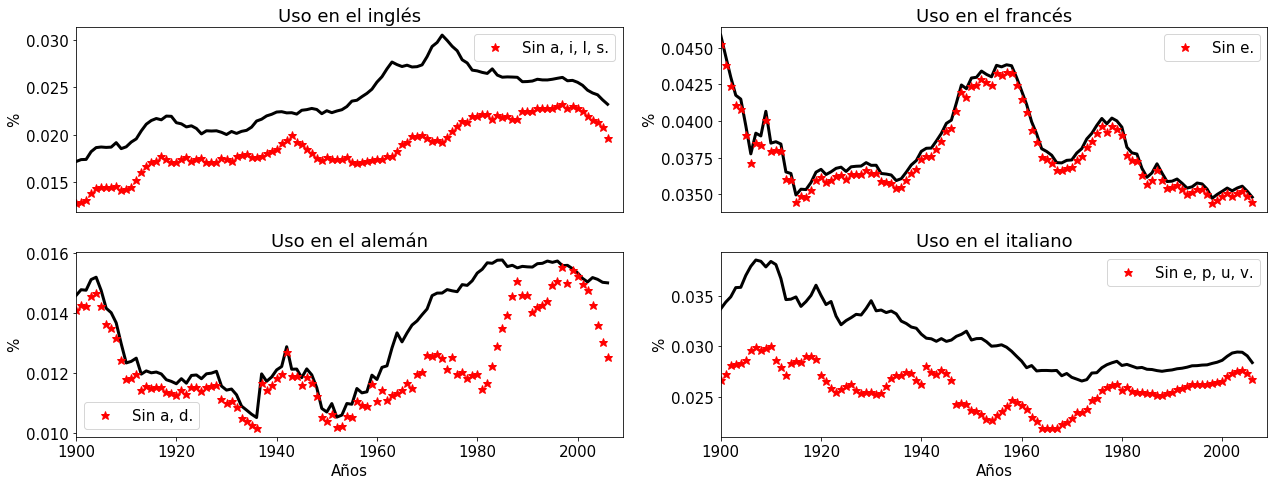
\includegraphics[scale=.375]{Cap_5/OM_SP.png}
	\label{fig.OM_SP}
	\caption{Omisiones del español en los demás}
\end{figure}
            % ~5 páginas - Resumir lo que se hizo y lo que no y comentar trabajos futuros sobre el tema
\chapter{Diversidad de Rango}

Los primeros análisis se enfocaron en buscar hechos relevantes que propiciaron las migraciones de palabras,  siendo oportuna la información histórica.  El capítulo anterior busco ver a cada idioma como un conjunto “universal” donde las propiedades que lo caracterizan  son comunes en cada uno y siguen siendo válidas a pesar de reducir los elementos que los componen al extraer palabras. 

En esta sección se buscará entender cómo son las variaciones de palabras a  lo largo del tiempo, para ello  se enfocara el estudio a cuantificar que tan diferentes son las listas de los préstamos de un idioma en otro,  ya que estas listas están ordenadas por rango, (donde el rango más bajo es la palabra más común en ese año y la de rango más alto la menos utilizada)  una misma palabra puede ocupar distintos cargos en diferentes años,  o  para un mismo rango existe una diversidad de palabras que lo ocupan, esta idea es más adecuada ya hay palabras que no  aparecen en todos los años del análisis,  sin embargo en todos las listas  hay palabras hasta cierta posición (rango).   

La propuesta de la diversidad de rango ha utilizada en idiomas y en deportes [XXXX], siendo útil para mostrar características comunes de los conjuntos donde es medida.  El algoritmo para llegar a la diversidad se propuso en [XXX], y se describe de la siguiente manera:


\begin{enumerate}
	
	\item Se fijan un año inicial $t_{o}$ y uno final $t_{o}$, construyendo un intervalo de años a evaluar $\Delta\,t = t_{f}- t_{o}$.
	
	\item Se toma el primer rango de todos los años en el intervalo y se cuenta el número de palabras que son distintas en ese rango. Esta cantidad será la diversidad para el rango uno.
	
	\item Se prosigue con el segundo rango y se vuelve a contar cuántas palabras son diferentes en todo el periodo de tiempo.  Con ello se obtiene la diversidad para el rango dos. 
	
	\item Ya que las listas de préstamos de un idioma en otro no son homogéneas en cantidad, el procedimiento anterior se repetirá hasta el rango mínimo que poseen todas las listas,  así se asegura tener una homogeneidad en el tamaño.
	
	\item Se normalizan  los valores dividiendo cada resultado entre el número de años comprendidos del intervalo $\Delta\,t$, obteniendo  la diversidad de rango $d(k)$.
	
	
\end{enumerate}


Antes de mostrar los resultados, se espera  que los valores de $d(k)$ sean cercanos a cero cuando  para un rango $k$, las cantidad de palabras que ocupan ese rango sea menor. En caso de que la diversidad sea cercana a uno,  significa que hay una mayor cantidad de palabras que ocupan el rango $k$. 


Tras graficar el rango contra la diversidad, se observó que en todas las combinaciones (a pesar de que algunas tuvieran más datos)  la tendencia de la diversidad  se asemeja a una función de distribución cumulativa logarítmica  normal, la cual depende del rango $k$, y la desviación estándar $\sigma$.

\begin{equation}
	\label{ec.cumulativa}
	F(k) = \Phi \left ( \frac{ln(k)}{\sigma} \right )\,\,\,\,k\geq 0; \sigma \geq 0
\end{equation}

Donde $\Phi$ es la función cumulativa de la distribución normal, que ademas del rango y la desviación estándar, depende del promedio $\mu$.

\begin{equation}
	\label{ec.distribucionnormal}
	\Phi(t) = \frac{1}{\sigma\sqrt{2\pi}} \int_{-\infty}^{t}  e^{ \frac{ - \left ( x-\mu \right )^{2}}{2\sigma^2}  } dx	
\end{equation}


\newpage
\subsubsection*{Ajuste de Datos }


Se intentó ajustar los puntos de la diversidad con esta distribución, sin embargo al ser pocos los rangos (la mayor cantidad de rangos en cualquier combinación fue de 250),  la curva descrita  no ajusta correctamente;  si se tuvieran mayor cantidad de rangos (1000 o 1000) del orden de $10^{3}$ o $10^{4}$ el ajuste es más preciso.  Para solucionar este problema se propuso hacer un ajuste lineal con la función logarítmica  de la siguiente forma:


\begin{enumerate}
	\item Se propone una función para la diversidad $d(k)$ de la forma
	
	\begin{equation}
	\label{ec.ajuste}
	y(k) =  \alpha \, ln(k) + \beta
	\end{equation}
	
	\item Al realizar los cambios de variable $\hat{Y} = y(k)$ y $X = ln(k)$, se obtiene una ecuación lineal para $k$.
	$$ \hat{Y} =  \alpha X + \beta$$
	
	\item Para encontrar los parámetros $\alpha$ y $\beta$, se utilizó el método de mínimos cuadrados, minimizando la suma de los cuadrados de los errores.  
	
	\item Conocidos los valores de $X$, la diversidad $Y$ y la cantidad de valores $n$,  se calcularon los valores muestrales de las medias ($\mu_{X}$ y $\mu_{Y}$), las varianzas ($\sigma^{2}_{X}$ $\sigma^{2}_{Y}$)  y la covarianza de las dos variables  $\sigma_{XY}$.
	
	$$ \bar{X} = \frac{1}{n} \sum_{i=1}^{n} X_{i} $$
	
	$$ \bar{Y} = \frac{1}{n} \sum_{i=1}^{n} Y_{i} $$
	
	$$ \sigma^{2}_{X} = \frac{1}{n} \sum_{i=1}^{n} \left (X_{i} -\bar{X}\right )^{2} $$
	
	$$ \sigma^{2}_{Y} = \frac{1}{n} \sum_{i=1}^{n} \left (Y_{i} -\bar{Y}\right )^{2} $$
	
	$$ \sigma_{XY} = \frac{1}{n} \sum_{i=1}^{n} \left (X_{i} - \bar{X}\right )  \left (Y_{i} - \bar{Y} \right ) $$
	
	\item Así los parámetros se expresan como
	
	$$ \alpha = \frac{\sigma_{XY}}{\sigma^{2}_{X}} $$
	
	$$ \beta = \bar{Y} - \alpha \bar{X}$$
	
	\item Calculados cada punto del ajuste (\ref{ec.ajuste}) $y_{i}$ y los valores calculados de diversidad $f_{i}$, para comprobar que tan adecuado es el ajuste se obtiene el coeficiente de determinación $R^{2}$.
	
	\begin{equation}
	\label{ec.rcuadrado}
	R^{2} = \frac{\sigma_{XY}}{\sigma^{2}_{X} \sigma^{2}_{Y}} \,\, = \,\, 1- \frac{\sum_{i=1}^{n} \left( y_{i} - f_{i}\right)^{2} }{\sum_{i=1}^{n} \left (y_{i} -\bar{Y}\right )^{2}}
	\end{equation}
	
	
	 
\end{enumerate}


Valores de $R^{2}$ próximos a 1 indicarán que existe una relación lineal ( en este caso logarítmica por el cambio de variable) exacta entre las dos variables

Las posteriores gráficas corresponden a las diferentes combinaciones entre idiomas orígenes y los receptores donde se calculó la diversidad de rango y el ajuste correspondiente.  Por cada conjunto de gráficas se muestra una tabla con los diferentes parámetros, la media $\mu$, la desviación estándar $\sigma$, el rango minimo donde se buscó la diversidad $k_{min}$, los parámetros del ajuste $\alpha$ y $\beta$  y el coeficiente de determinación $R^{2}$.
 
\newpage

\begin{figure}[h!]
	\centering
	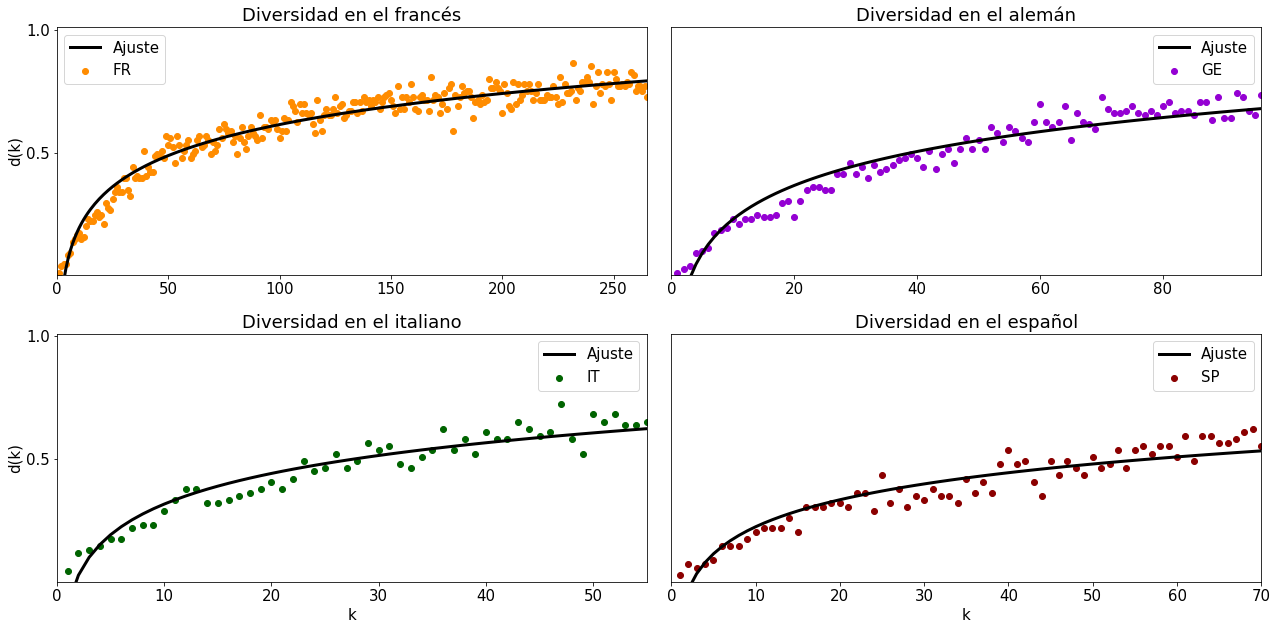
\includegraphics[width=15cm, height=6.8cm]{Cap_6/DR_EN.png}
	\label{fig.DR_EN}
	\caption{Diversidad de rango del inglés en los demás.}
\end{figure}


\begin{table}[h!]
	\centering
	\begin{tabular}{ccccccc}
		\textbf{}                & \textbf{$\mu$} & \textbf{$\sigma$} & \textbf{$k_{min}$} & \textbf{$\alpha$} & \textbf{$\beta$} & \textbf{$R^{2}$} \\
		\textbf{inglés-francés}  & 0.61           & 0.18                & 265                   & 0.18           & -0.23         & 0.94        \\
		\textbf{inglés-alemán}   & 0.49           & 0.19                & 96                    & 0.19           & -0.23         & 0.92        \\
		\textbf{ingles-italiano} & 0.45           & 0.17                & 55                    & 0.17           & -0.10         & 0.91        \\
		\textbf{ingles-español}  & 0.38           & 0.15                & 70                    & 0.15           & -0.14         & 0.88       
	\end{tabular}
	\caption{Parámetros de la diversidad del inglés en los demás.}
	\label{tab.DR_EN}
\end{table}



\newpage

\begin{figure}[h!]
	\centering
	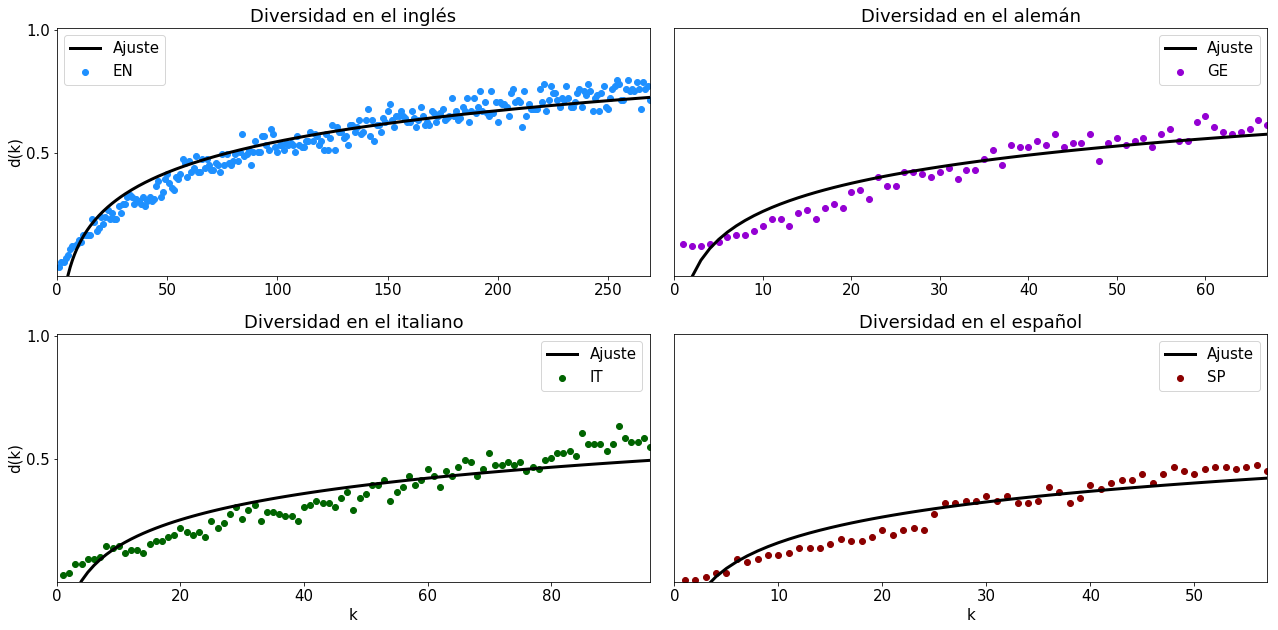
\includegraphics[width=1 \textwidth, scale = .38]{Cap_6/DR_FR.png}
	\label{fig.DR_FR}
	\caption{Diversidad de rango del francés en los demás.}
\end{figure}


\begin{table}[h!]
	\centering
	\begin{tabular}{ccccccc}
		\textbf{}                & \textbf{$\mu$} & \textbf{$\sigma$} & \textbf{$k_{min}$} & \textbf{$\alpha$} & \textbf{$\beta$} & \textbf{$R^{2}$} \\
		\textbf{francés-inglés}  & 0.55           & 0.18                & 269                   & 0.18           & -0.29        & 0.93        \\
		\textbf{francés-alemán}   & 0.42           & 0.16                & 67                    & 0.17           & -0.12         & 0.87        \\
		\textbf{francés-italiano} & 0.35           & 0.16                & 96                    & 0.15           & -0.21         & 0.83        \\
		\textbf{francés-español}  & 0.28           & 0.14                & 57                    & 0.15           & -0.19         & 0.86       
	\end{tabular}
	\caption{Parámetros de la diversidad del francés en los demás.}
	\label{tab.DR_FR}
\end{table}


\newpage

\begin{figure}[h!]
	\centering
	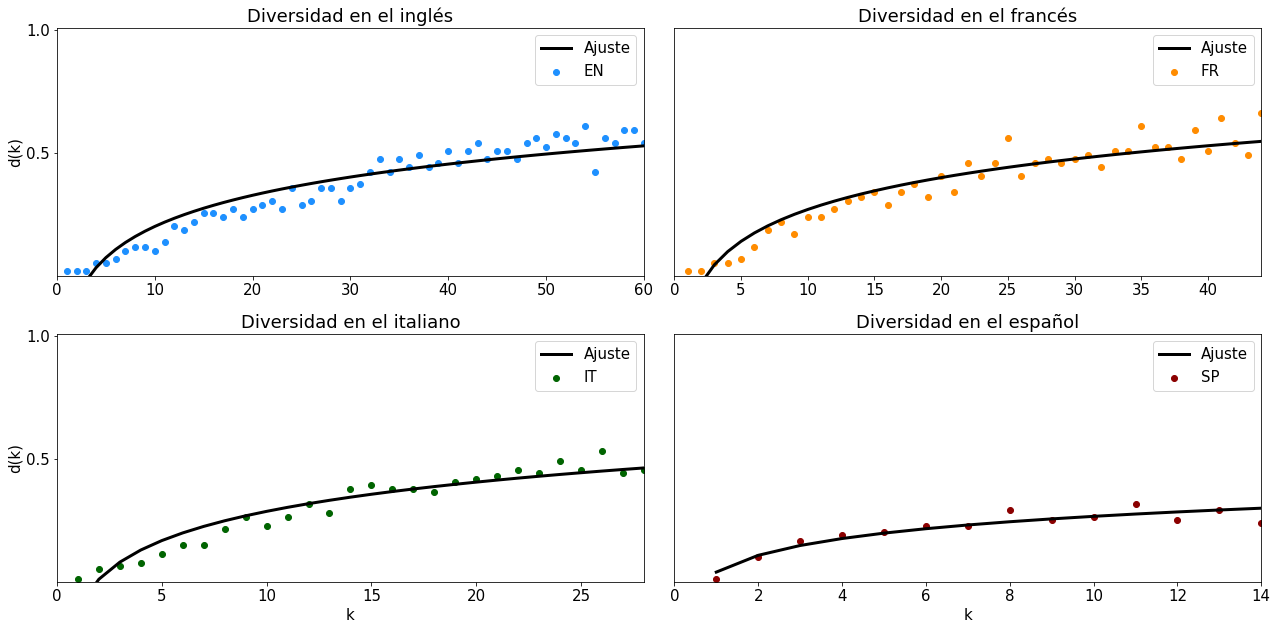
\includegraphics[width=1 \textwidth, scale = .38]{Cap_6/DR_GE.png}
	\label{fig.DR_GE}
	\caption{Diversidad de rango del alemán en los demás.}
\end{figure}


\begin{table}[h!]
	\centering
	\begin{tabular}{ccccccc}
		\textbf{}                & \textbf{$\mu$} & \textbf{$\sigma$} & \textbf{$k_{min}$} & \textbf{$\alpha$} & \textbf{$\beta$} & \textbf{$R^{2}$} \\
		\textbf{alemán-inglés}  & 0.35          & 0.17                & 60                   & 0.18           & -0.22        & 0.88        \\
		\textbf{alemán-francés}   & 0.37           & 0.17                & 44                    & 0.19           & -0.16         & 0.89        \\
		\textbf{alemán-italiano} & 0.31           & 0.15                & 28                    & 0.17           & -0.11         & 0.91        \\
		\textbf{alemán-español}  & 0.22          & 0.08                & 14                    & 0.10           & -0.04         & 0.89       
	\end{tabular}
	\caption{Parámetros de la diversidad del alemán en los demás.}
	\label{tab.DR_GE}
\end{table}


\newpage

\begin{figure}[h!]
	\centering
	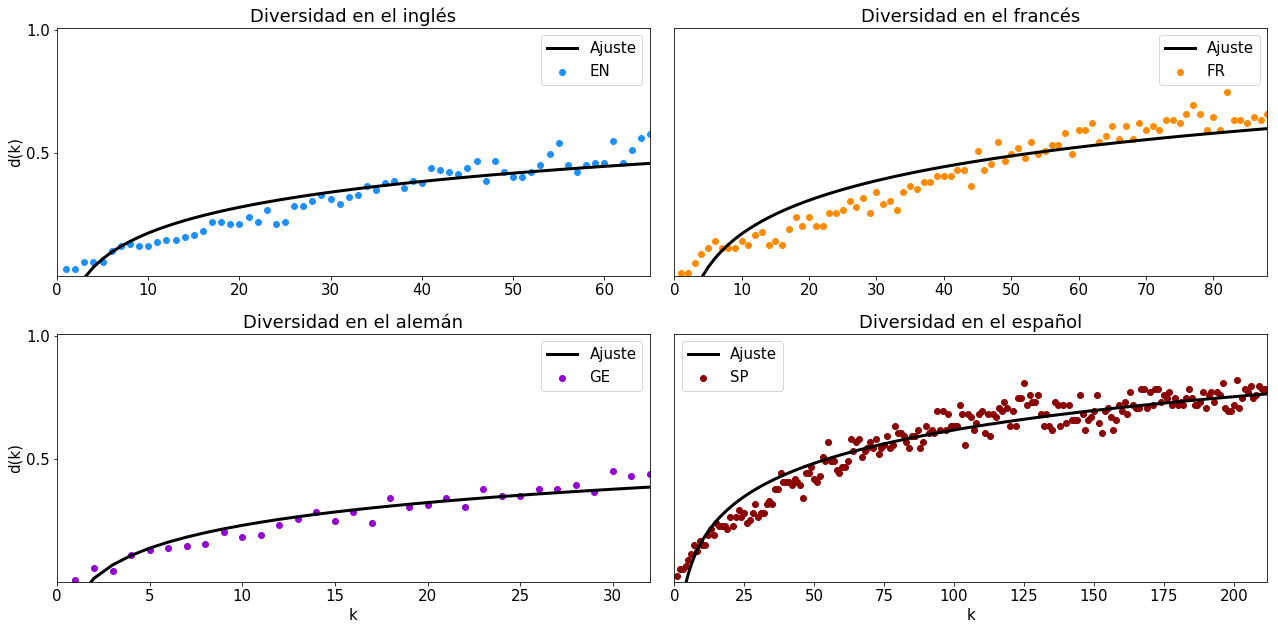
\includegraphics[width=1 \textwidth, scale = .38]{Cap_6/DR_IT.png}
	\label{fig.DR_IT}
	\caption{Diversidad de rango del italiano en los demás.}
\end{figure}


\begin{table}[h!]
	\centering
	\begin{tabular}{ccccccc}
		\textbf{}                & \textbf{$\mu$} & \textbf{$\sigma$} & \textbf{$k_{min}$} & \textbf{$\alpha$} & \textbf{$\beta$} & \textbf{$R^{2}$} \\
		\textbf{italiano-inglés}  & 0.31          & 0.15                & 66                   & 0.15           & -0.18        & 0.86        \\
		\textbf{italiano-francés}   & 0.41           & 0.20                & 88                    & 0.20           & -0.28         & 0.85        \\
		\textbf{italiano-alemán} & 0.26           & 0.12                & 32                    & 0.13           & -0.08         & 0.91        \\
		\textbf{italiano-español}  & 0.22          & 0.19                & 212                    & 0.20           & -0.28         & 0.92       
	\end{tabular}
	\caption{Parámetros de la diversidad del italiano en los demás.}
	\label{tab.DR_IT}
\end{table}


\newpage

\begin{figure}[h!]
	\centering
	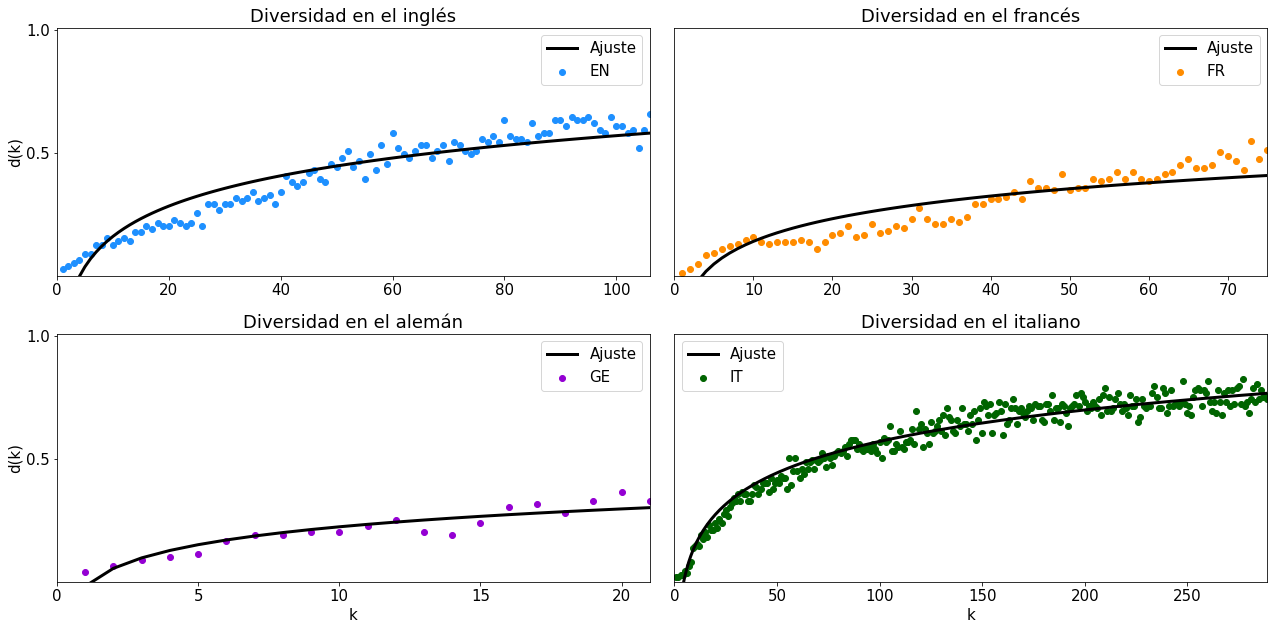
\includegraphics[width=1 \textwidth, scale = .38]{Cap_6/DR_SP.png}
	\label{fig.DR_SP}
	\caption{Diversidad de rango del español en los demás.}
\end{figure}


\begin{table}[h!]
	\centering
	\begin{tabular}{ccccccc}
		\textbf{}                & \textbf{$\mu$} & \textbf{$\sigma$} & \textbf{$k_{min}$} & \textbf{$\alpha$} & \textbf{$\beta$} & \textbf{$R^{2}$} \\
		\textbf{español-inglés}  & 0.41          & 0.18                & 106                   & 0.18           & -0.25        & 0.87        \\
		\textbf{español-francés}   & 0.28           & 0.14                & 75                   & 0.13           & -0.17         & 0.79        \\
		\textbf{español-alemán} & 0.21           & 0.09                & 21                    & 0.11           & -0.02         & 0.86        \\
		\textbf{español-italiano}  & 0.22          & 0.18                & 289                    & 0.18           & -0.28         & 0.95       
	\end{tabular}
	\caption{Parámetros de la diversidad del español en los demás.}
	\label{tab.DR_SP}
\end{table} 

\chapter{Conclusiones}
%%%%%%%%%%%%%%%%%%%%%%%%%%%%%%%%%%%%%%%%%%%%%%%%%%%%%
%                   APÉNDICES                       %
%%%%%%%%%%%%%%%%%%%%%%%%%%%%%%%%%%%%%%%%%%%%%%%%%%%%%
\appendix

% this file is called up by thesis.tex
% content in this file will be fed into the main document
\chapter{Complementos}
% top level followed by section, subsection

\section{Lectura de listas}

\newpage

\section{Gráficas de palabras nuevas entre dos idiomas}

\begin{figure}[h!]
	\centering
	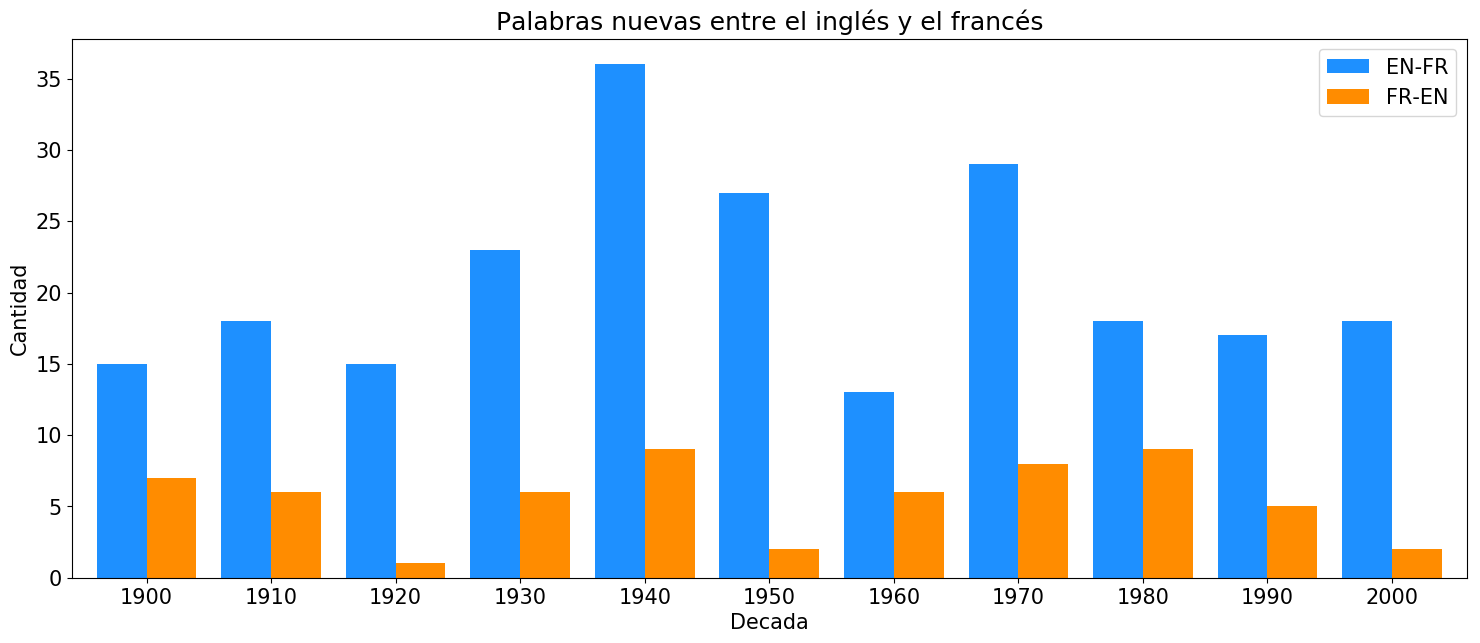
\includegraphics[scale=.38]{Cap_3/NC_1_S2_EN.png}
	\label{fig.NC_EF}
	\caption{Palabras nuevas entre el inglés y el francés}
\end{figure}

\begin{figure}[h!]
	\centering
	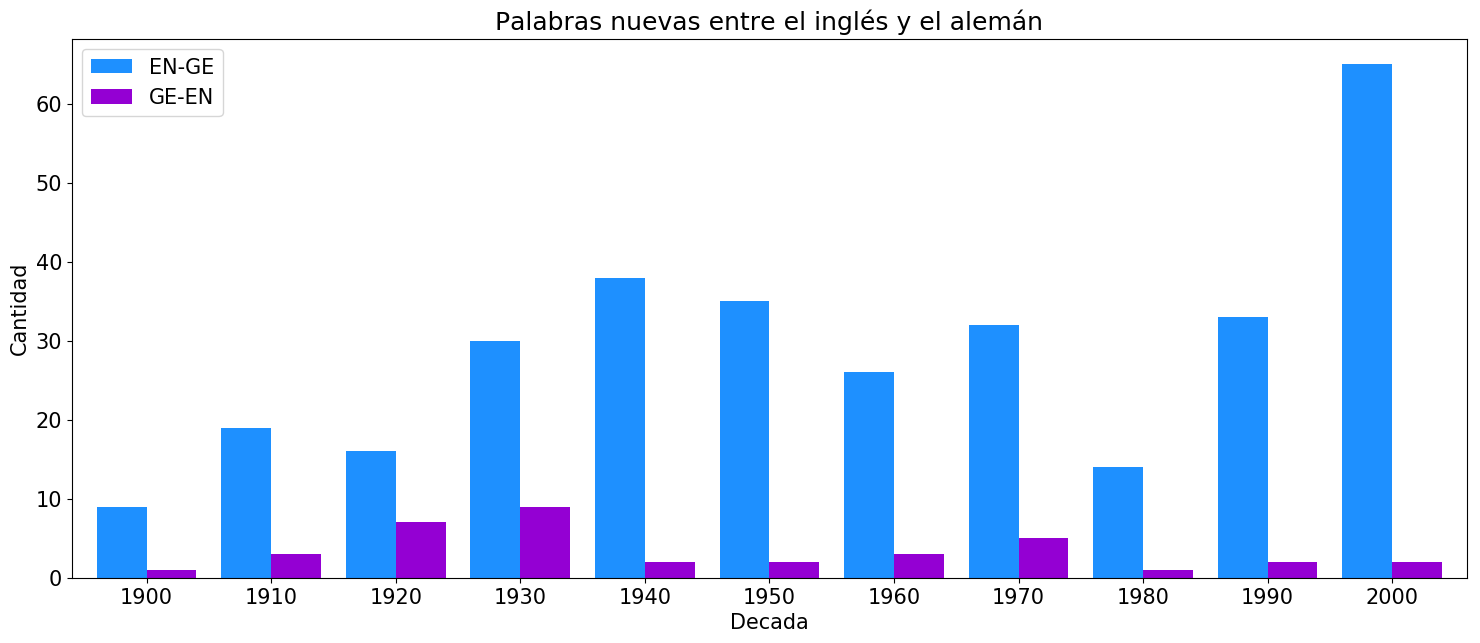
\includegraphics[scale=.38]{Cap_3/NC_2_S2_EN.png}
	\label{fig.NC_EG}
	\caption{Palabras nuevas entre el inglés y el alemán}
\end{figure}

\begin{figure}[h!]
	\centering
	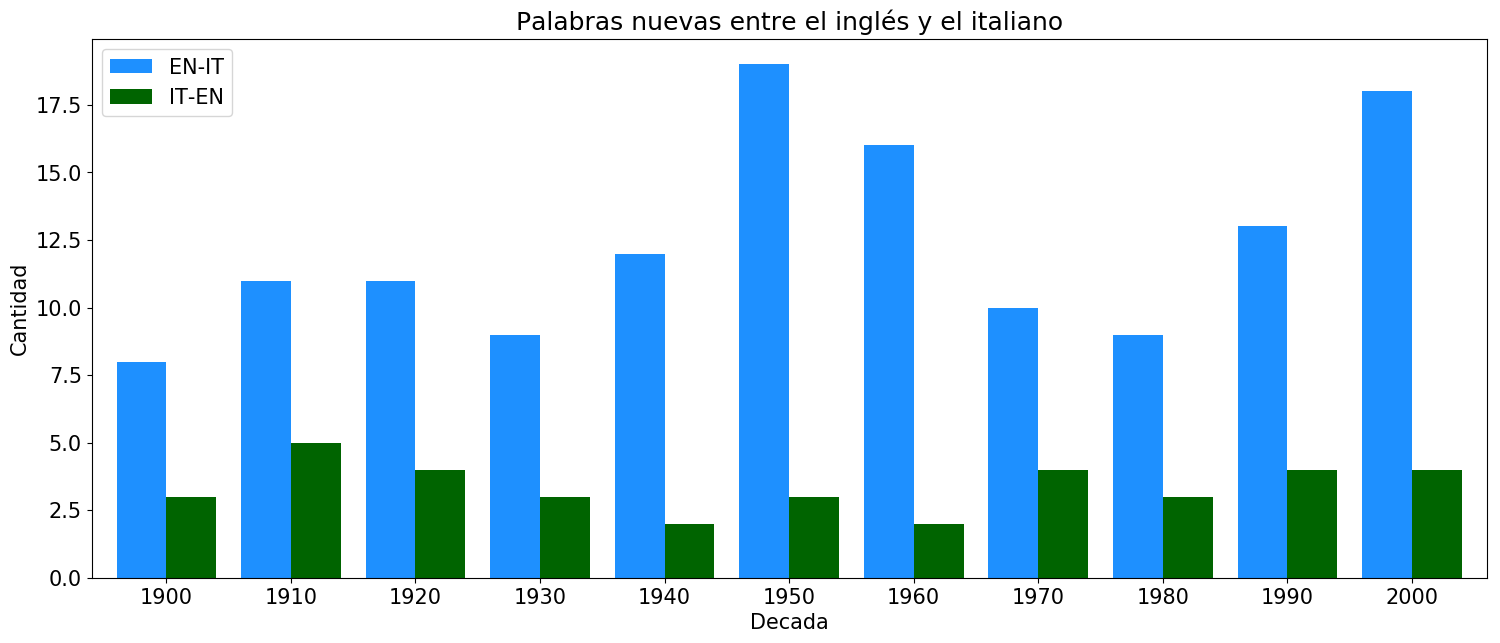
\includegraphics[scale=.38]{Cap_3/NC_3_S2_EN.png}
	\label{fig.NC_EI}
	\caption{Palabras nuevas entre el inglés y el italiano}
\end{figure}


\begin{figure}[h!]
	\centering
	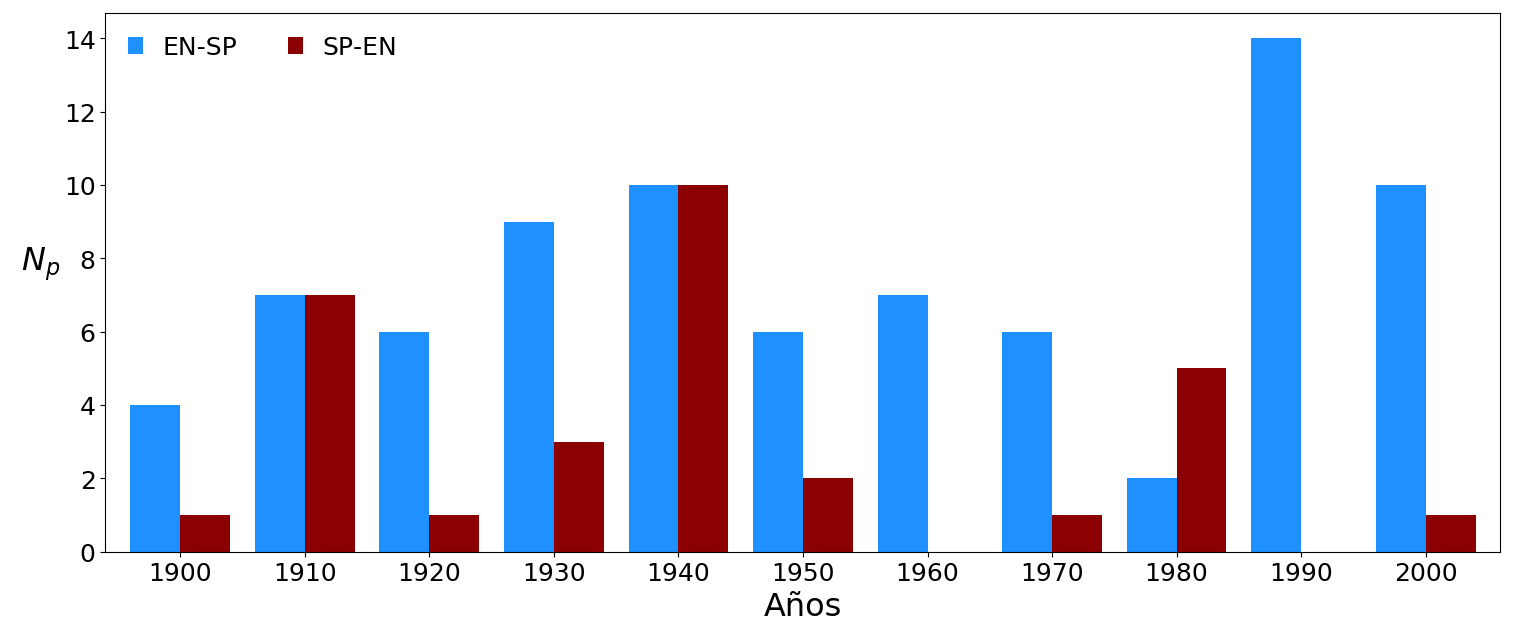
\includegraphics[scale=.38]{Cap_3/NC_4_S2_EN.png}
	\label{fig.NC_ES}
	\caption{Palabras nuevas entre el inglés y el español}
\end{figure}

\begin{figure}[h!]
	\centering
	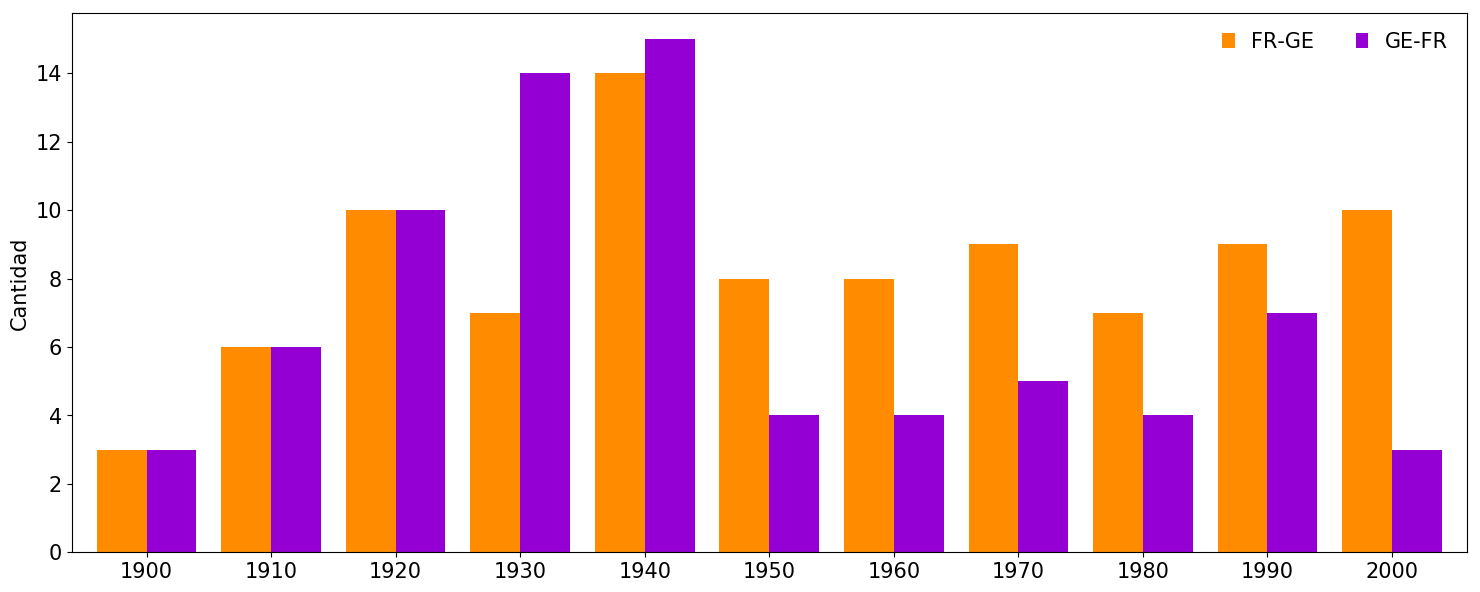
\includegraphics[scale=.38]{Cap_3/NC_2_S2_FR.png}
	\label{fig.NC_FG}
	\caption{Palabras nuevas entre el francés y el alemán}
\end{figure}


\begin{figure}[h!]
	\centering
	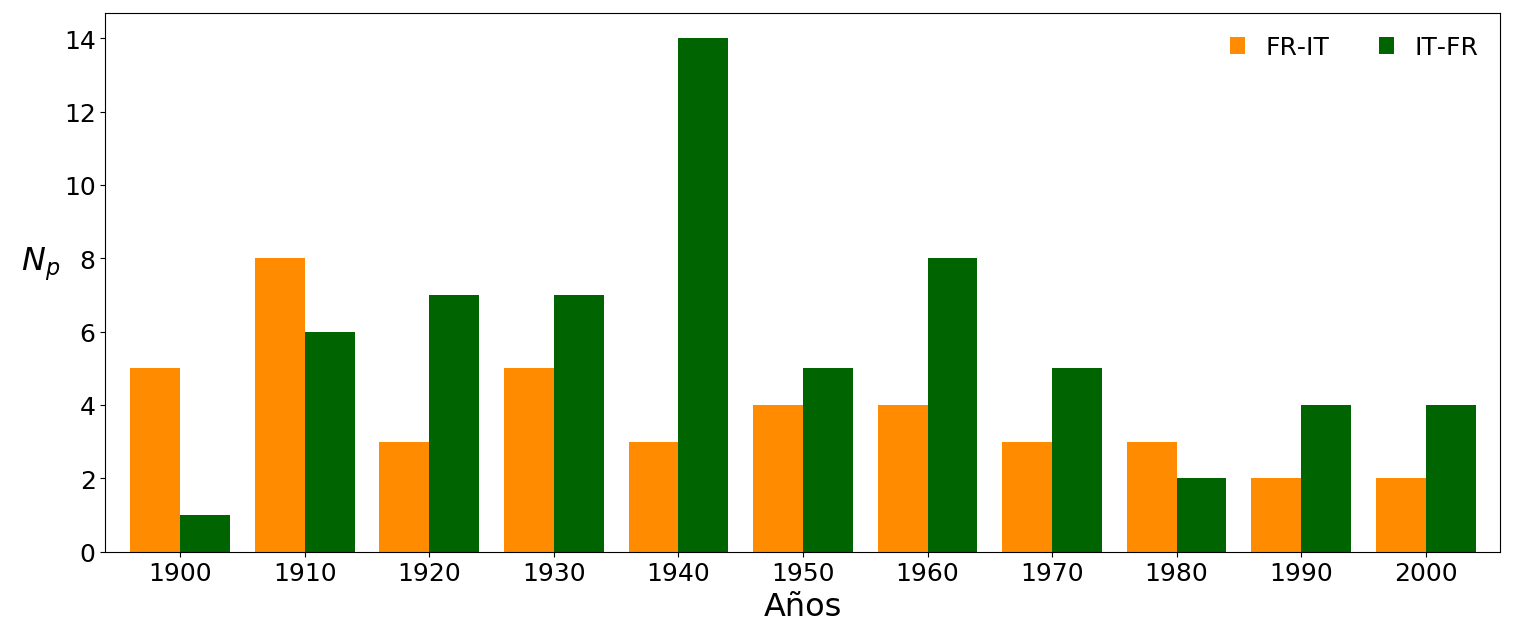
\includegraphics[scale=.38]{Cap_3/NC_3_S2_FR.png}
	\label{fig.NC_FI}
	\caption{Palabras nuevas entre el francés y el italiano}
\end{figure}

\begin{figure}[h!]
	\centering
	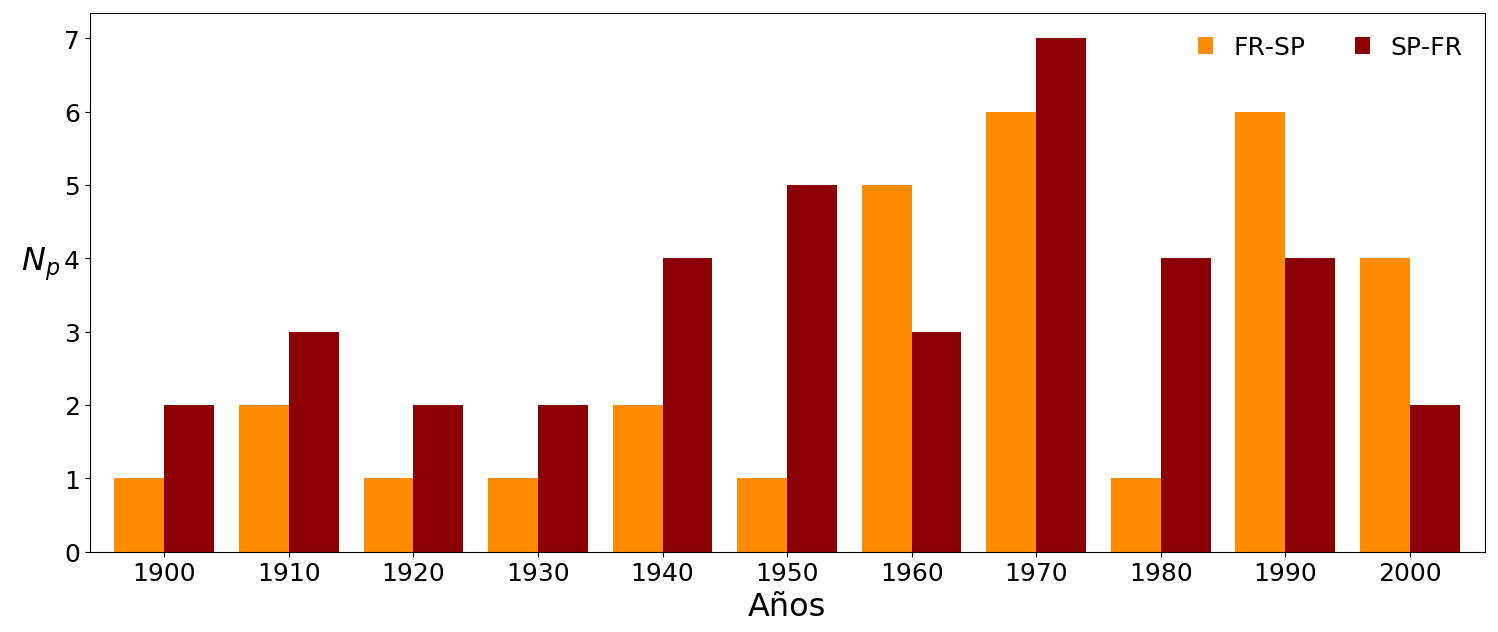
\includegraphics[scale=.38]{Cap_3/NC_4_S2_FR.png}
	\label{fig.NC_FS}
	\caption{Palabras nuevas entre el francés y el español}
\end{figure}

\begin{figure}[h!]
	\centering
	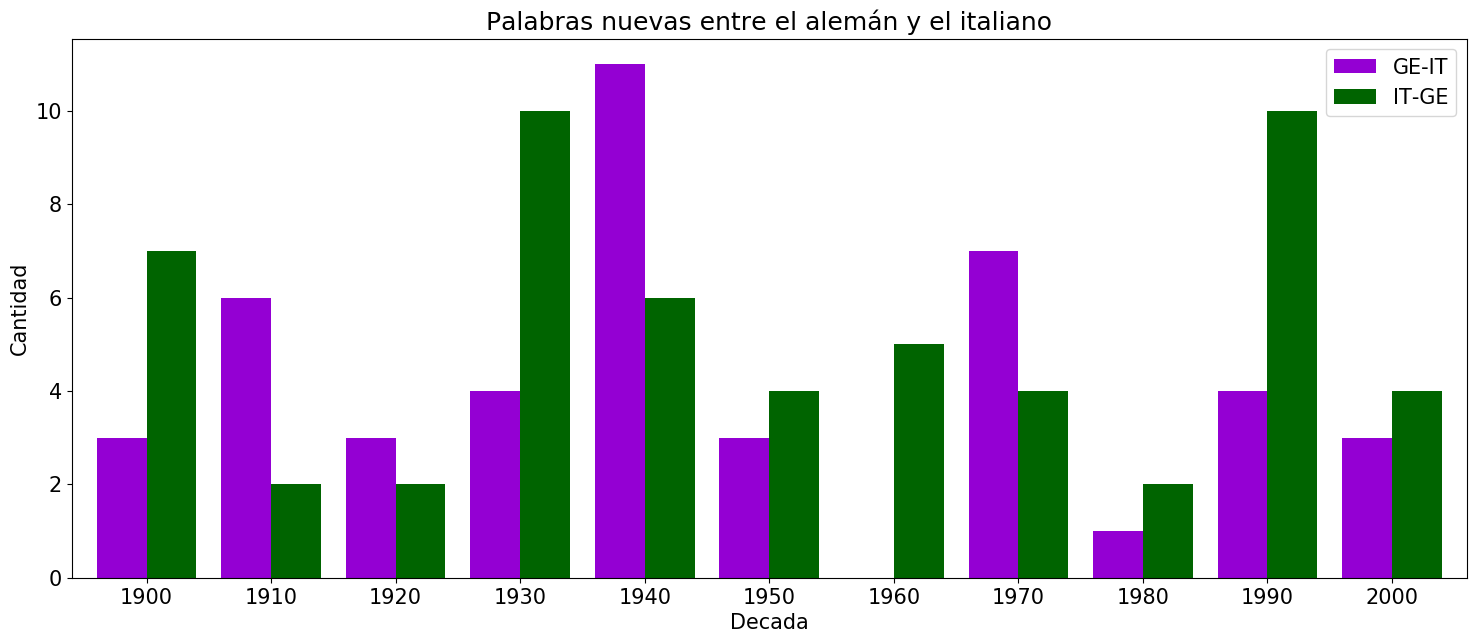
\includegraphics[scale=.38]{Cap_3/NC_3_S2_GE.png}
	\label{fig.NC_GI}
	\caption{Palabras nuevas entre el alemán y el italiano}
\end{figure}

\begin{figure}[h!]
	\centering
	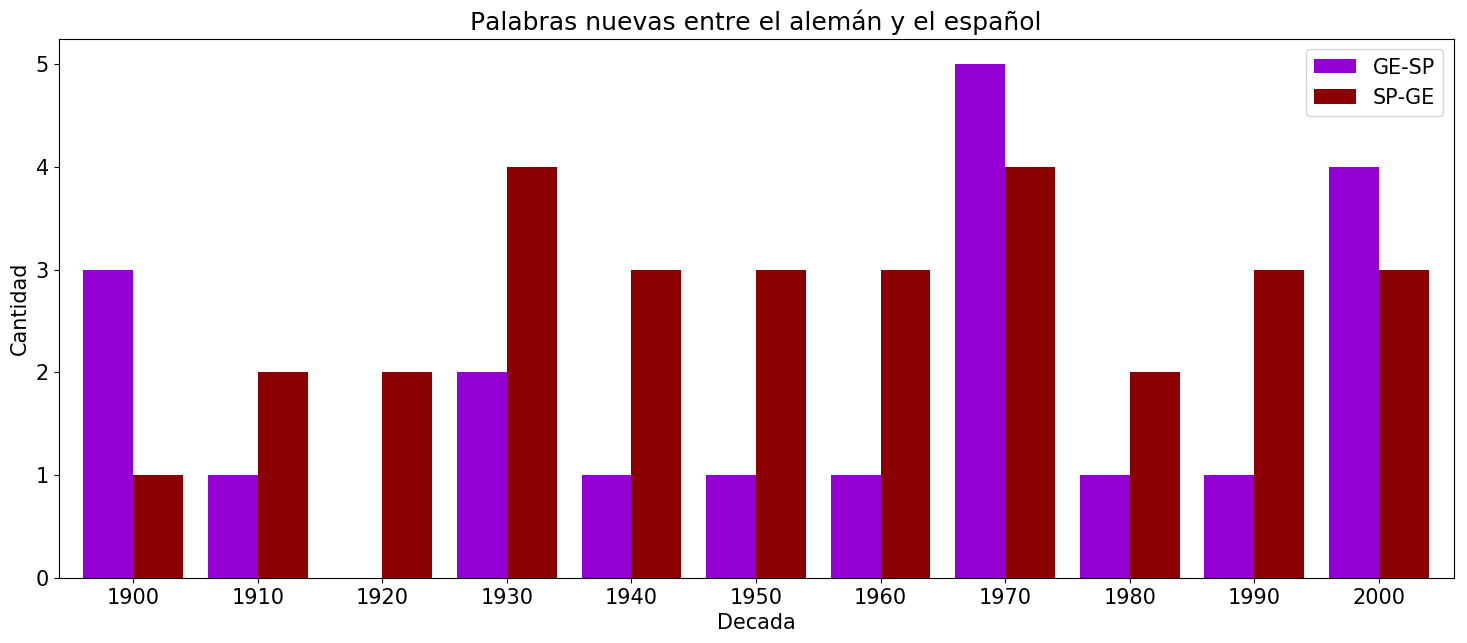
\includegraphics[scale=.38]{Cap_3/NC_4_S2_GE.png}
	\label{fig.NC_GS}
	\caption{Palabras nuevas entre el alemán y el español}
\end{figure}

\begin{figure}[h!]
	\centering
	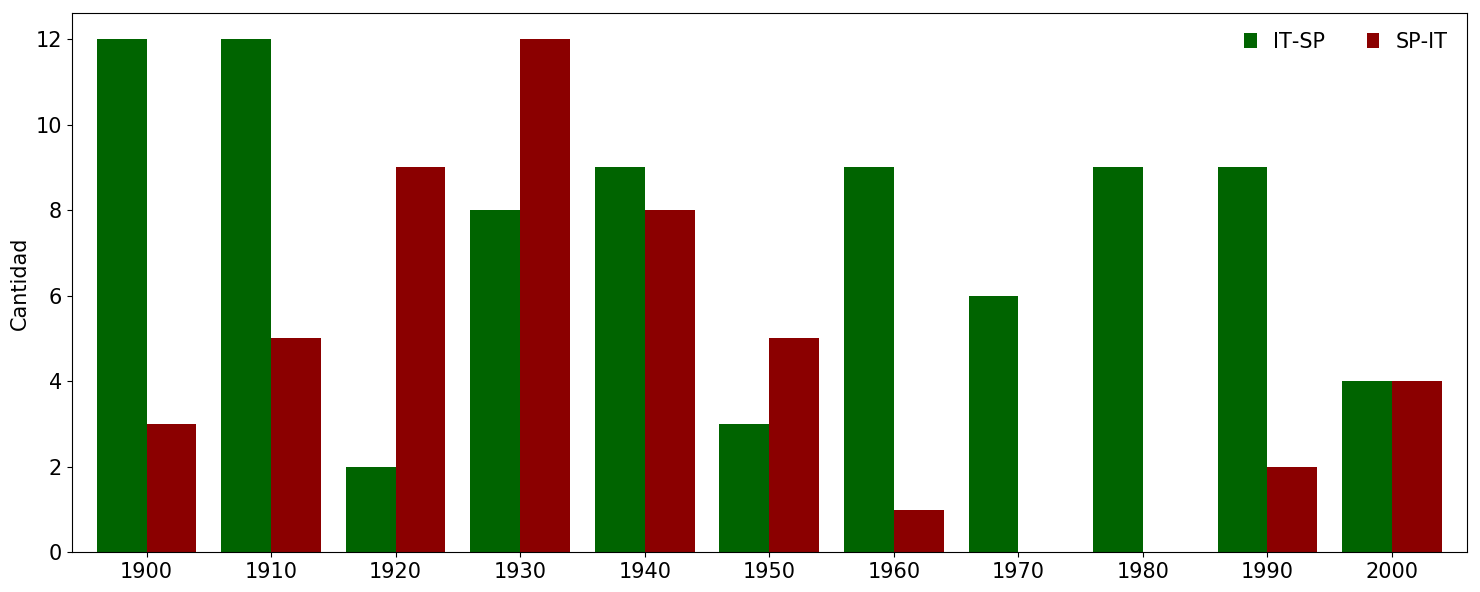
\includegraphics[scale=.38]{Cap_3/NC_4_S2_IT.png}
	\label{fig.NC_IS}
	\caption{Palabras nuevas entre el italiano y el español}
\end{figure}

\newpage


\section{Gráficas de palabras acumuladas entre dos idiomas}

\begin{figure}[h!]
	\centering
	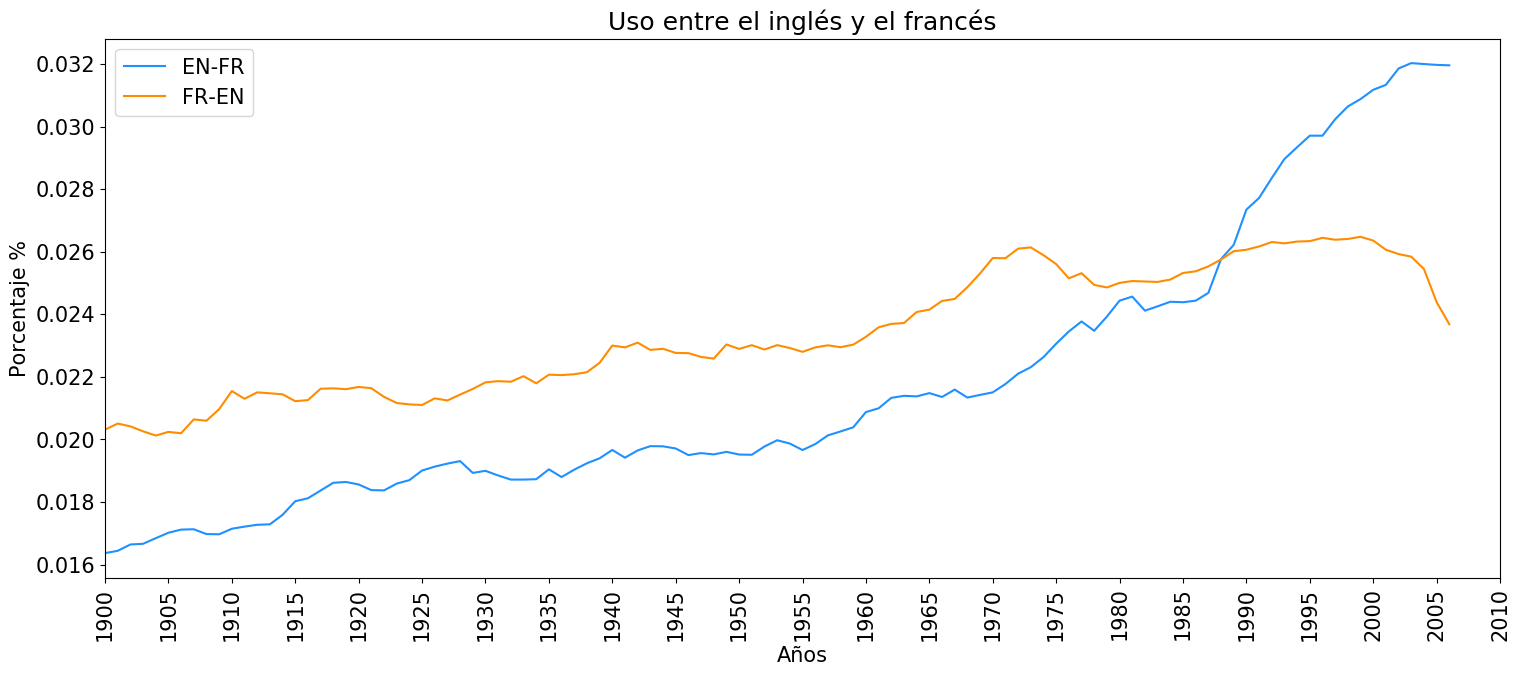
\includegraphics[scale=.38]{Cap_4/SF_1_S2_EN.png}
	\label{fig.SF_EF}
	\caption{Palabras acumuladas entre el inglés y el francés}
\end{figure}


\begin{figure}[h!]
	\centering
	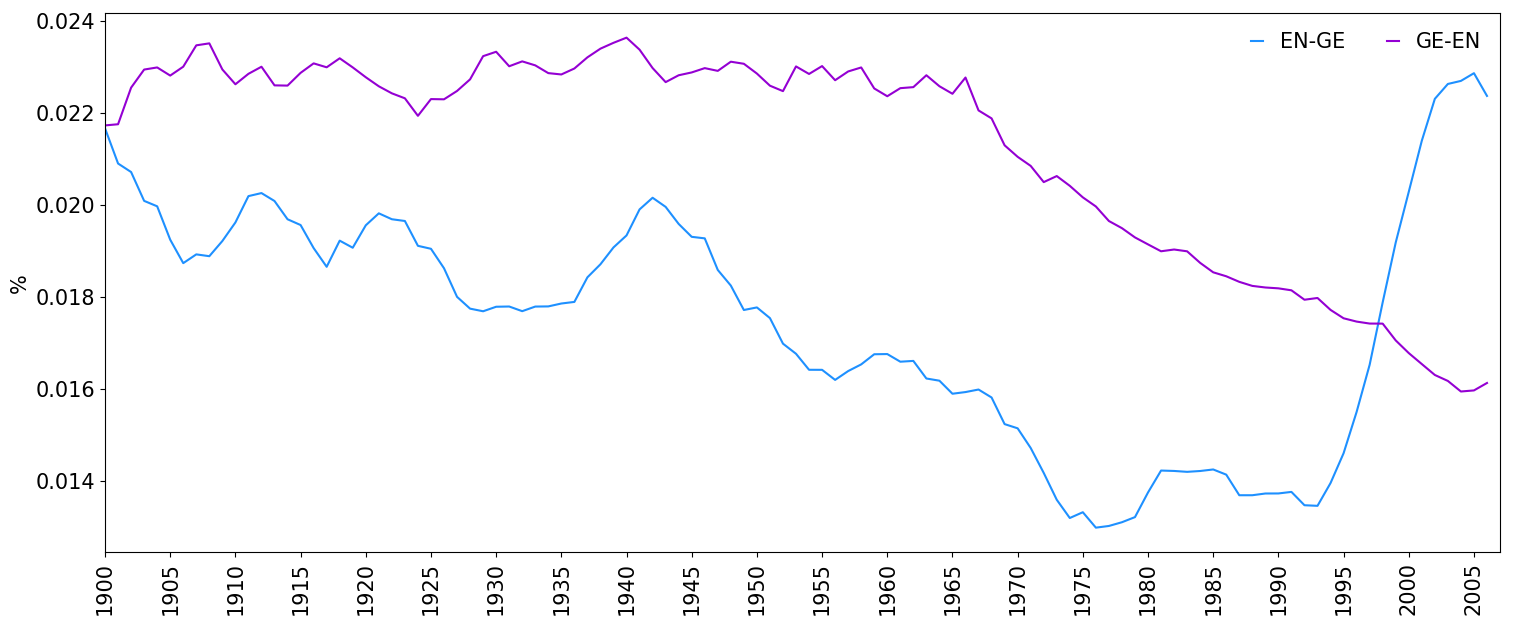
\includegraphics[scale=.38]{Cap_4/SF_2_S2_EN.png}
	\label{fig.SF_EG}
	\caption{Palabras acumuladas entre el inglés y el alemán}
\end{figure}


\begin{figure}[h!]
	\centering
	\includegraphics[scale=.38]{Cap_4/SF_3_S2_EN.png}
	\label{fig.SF_EI}
	\caption{Palabras acumuladas entre el inglés y el italiano}
\end{figure}

\begin{figure}[h!]
	\centering
	\includegraphics[scale=.38]{Cap_4/SF_4_S2_EN.png}
	\label{fig.SF_ES}
	\caption{Palabras acumuladas entre el inglés y el español}
\end{figure}

\begin{figure}[h!]
	\centering
	\includegraphics[scale=.38]{Cap_4/SF_2_S2_FR.png}
	\label{fig.SF_FG}
	\caption{Palabras acumuladas entre el francés y el alemán}
\end{figure}

\begin{figure}[h!]
	\centering
	\includegraphics[scale=.38]{Cap_4/SF_3_S2_FR.png}
	\label{fig.SF_FI}
	\caption{Palabras acumuladas entre el francés y el italiano}
\end{figure}

\begin{figure}[h!]
	\centering
	\includegraphics[scale=.38]{Cap_4/SF_4_S2_FR.png}
	\label{fig.SF_FS}
	\caption{Palabras acumuladas entre el francés y el español}
\end{figure}



\begin{figure}[h!]
	\centering
	\includegraphics[scale=.38]{Cap_4/SF_3_S2_GE.png}
	\label{fig.SF_GI}
	\caption{Palabras acumuladas entre el alemán y el italiano}
\end{figure}


\begin{figure}[h!]
	\centering
	\includegraphics[scale=.38]{Cap_4/SF_4_S2_GE.png}
	\label{fig.SF_GS}
	\caption{Palabras acumuladas entre el alemán y el español}
\end{figure}


\begin{figure}[h!]
	\centering
	\includegraphics[scale=.38]{Cap_4/SF_4_S2_IT.png}
	\label{fig.SF_IE}
	\caption{Palabras acumuladas entre el italiano y el español}
\end{figure}
               % Colocar los circuitos, manuales, código fuente, pruebas de teoremas, etc.

%%%%%%%%%%%%%%%%%%%%%%%%%%%%%%%%%%%%%%%%%%%%%%%%%%%%%
%                   REFERENCIAS                     %
%%%%%%%%%%%%%%%%%%%%%%%%%%%%%%%%%%%%%%%%%%%%%%%%%%%%%
% existen varios estilos de bilbiografía, pueden cambiarlos a placer
%\bibliographystyle{apalike} % otros estilos pueden ser abbrv, acm, alpha, apalike, ieeetr, plain, siam, unsrt

%El formato trae otros estilos, o pueden agregar uno que les guste:
%\bibliographystyle{Latex/Classes/PhDbiblio-case} % title forced lower case
%\bibliographystyle{Latex/Classes/PhDbiblio-bold} % title as in bibtex but bold
\bibliographystyle{Latex/Classes/PhDbiblio-url} % bold + www link if provided
%\bibliographystyle{Latex/Classes/jmb} % calls style file jmb.bst

\bibliography{Bibliografia/referencias}             % Archivo .bib


\end{document}
